\documentclass[11pt]{article}

    \usepackage[breakable]{tcolorbox}
    \usepackage{parskip} % Stop auto-indenting (to mimic markdown behaviour)
    

    % Basic figure setup, for now with no caption control since it's done
    % automatically by Pandoc (which extracts ![](path) syntax from Markdown).
    \usepackage{graphicx}
    % Maintain compatibility with old templates. Remove in nbconvert 6.0
    \let\Oldincludegraphics\includegraphics
    % Ensure that by default, figures have no caption (until we provide a
    % proper Figure object with a Caption API and a way to capture that
    % in the conversion process - todo).
    \usepackage{caption}
    \DeclareCaptionFormat{nocaption}{}
    \captionsetup{format=nocaption,aboveskip=0pt,belowskip=0pt}

    \usepackage{float}
    \floatplacement{figure}{H} % forces figures to be placed at the correct location
    \usepackage{xcolor} % Allow colors to be defined
    \usepackage{enumerate} % Needed for markdown enumerations to work
    \usepackage{geometry} % Used to adjust the document margins
    \usepackage{amsmath} % Equations
    \usepackage{amssymb} % Equations
    \usepackage{textcomp} % defines textquotesingle
    % Hack from http://tex.stackexchange.com/a/47451/13684:
    \AtBeginDocument{%
        \def\PYZsq{\textquotesingle}% Upright quotes in Pygmentized code
    }
    \usepackage{upquote} % Upright quotes for verbatim code
    \usepackage{eurosym} % defines \euro

    \usepackage{iftex}
    \ifPDFTeX
        \usepackage[T1]{fontenc}
        \IfFileExists{alphabeta.sty}{
              \usepackage{alphabeta}
          }{
              \usepackage[mathletters]{ucs}
              \usepackage[utf8x]{inputenc}
          }
    \else
        \usepackage{fontspec}
        \usepackage{unicode-math}
    \fi

    \usepackage{fancyvrb} % verbatim replacement that allows latex
    \usepackage{grffile} % extends the file name processing of package graphics
                         % to support a larger range
    \makeatletter % fix for old versions of grffile with XeLaTeX
    \@ifpackagelater{grffile}{2019/11/01}
    {
      % Do nothing on new versions
    }
    {
      \def\Gread@@xetex#1{%
        \IfFileExists{"\Gin@base".bb}%
        {\Gread@eps{\Gin@base.bb}}%
        {\Gread@@xetex@aux#1}%
      }
    }
    \makeatother
    \usepackage[Export]{adjustbox} % Used to constrain images to a maximum size
    \adjustboxset{max size={0.9\linewidth}{0.9\paperheight}}

    % The hyperref package gives us a pdf with properly built
    % internal navigation ('pdf bookmarks' for the table of contents,
    % internal cross-reference links, web links for URLs, etc.)
    \usepackage{hyperref}
    % The default LaTeX title has an obnoxious amount of whitespace. By default,
    % titling removes some of it. It also provides customization options.
    \usepackage{titling}
    \usepackage{longtable} % longtable support required by pandoc >1.10
    \usepackage{booktabs}  % table support for pandoc > 1.12.2
    \usepackage{array}     % table support for pandoc >= 2.11.3
    \usepackage{calc}      % table minipage width calculation for pandoc >= 2.11.1
    \usepackage[inline]{enumitem} % IRkernel/repr support (it uses the enumerate* environment)
    \usepackage[normalem]{ulem} % ulem is needed to support strikethroughs (\sout)
                                % normalem makes italics be italics, not underlines
    \usepackage{soul}      % strikethrough (\st) support for pandoc >= 3.0.0
    \usepackage{mathrsfs}
    

    
    % Colors for the hyperref package
    \definecolor{urlcolor}{rgb}{0,.145,.698}
    \definecolor{linkcolor}{rgb}{.71,0.21,0.01}
    \definecolor{citecolor}{rgb}{.12,.54,.11}

    % ANSI colors
    \definecolor{ansi-black}{HTML}{3E424D}
    \definecolor{ansi-black-intense}{HTML}{282C36}
    \definecolor{ansi-red}{HTML}{E75C58}
    \definecolor{ansi-red-intense}{HTML}{B22B31}
    \definecolor{ansi-green}{HTML}{00A250}
    \definecolor{ansi-green-intense}{HTML}{007427}
    \definecolor{ansi-yellow}{HTML}{DDB62B}
    \definecolor{ansi-yellow-intense}{HTML}{B27D12}
    \definecolor{ansi-blue}{HTML}{208FFB}
    \definecolor{ansi-blue-intense}{HTML}{0065CA}
    \definecolor{ansi-magenta}{HTML}{D160C4}
    \definecolor{ansi-magenta-intense}{HTML}{A03196}
    \definecolor{ansi-cyan}{HTML}{60C6C8}
    \definecolor{ansi-cyan-intense}{HTML}{258F8F}
    \definecolor{ansi-white}{HTML}{C5C1B4}
    \definecolor{ansi-white-intense}{HTML}{A1A6B2}
    \definecolor{ansi-default-inverse-fg}{HTML}{FFFFFF}
    \definecolor{ansi-default-inverse-bg}{HTML}{000000}

    % common color for the border for error outputs.
    \definecolor{outerrorbackground}{HTML}{FFDFDF}

    % commands and environments needed by pandoc snippets
    % extracted from the output of `pandoc -s`
    \providecommand{\tightlist}{%
      \setlength{\itemsep}{0pt}\setlength{\parskip}{0pt}}
    \DefineVerbatimEnvironment{Highlighting}{Verbatim}{commandchars=\\\{\}}
    % Add ',fontsize=\small' for more characters per line
    \newenvironment{Shaded}{}{}
    \newcommand{\KeywordTok}[1]{\textcolor[rgb]{0.00,0.44,0.13}{\textbf{{#1}}}}
    \newcommand{\DataTypeTok}[1]{\textcolor[rgb]{0.56,0.13,0.00}{{#1}}}
    \newcommand{\DecValTok}[1]{\textcolor[rgb]{0.25,0.63,0.44}{{#1}}}
    \newcommand{\BaseNTok}[1]{\textcolor[rgb]{0.25,0.63,0.44}{{#1}}}
    \newcommand{\FloatTok}[1]{\textcolor[rgb]{0.25,0.63,0.44}{{#1}}}
    \newcommand{\CharTok}[1]{\textcolor[rgb]{0.25,0.44,0.63}{{#1}}}
    \newcommand{\StringTok}[1]{\textcolor[rgb]{0.25,0.44,0.63}{{#1}}}
    \newcommand{\CommentTok}[1]{\textcolor[rgb]{0.38,0.63,0.69}{\textit{{#1}}}}
    \newcommand{\OtherTok}[1]{\textcolor[rgb]{0.00,0.44,0.13}{{#1}}}
    \newcommand{\AlertTok}[1]{\textcolor[rgb]{1.00,0.00,0.00}{\textbf{{#1}}}}
    \newcommand{\FunctionTok}[1]{\textcolor[rgb]{0.02,0.16,0.49}{{#1}}}
    \newcommand{\RegionMarkerTok}[1]{{#1}}
    \newcommand{\ErrorTok}[1]{\textcolor[rgb]{1.00,0.00,0.00}{\textbf{{#1}}}}
    \newcommand{\NormalTok}[1]{{#1}}

    % Additional commands for more recent versions of Pandoc
    \newcommand{\ConstantTok}[1]{\textcolor[rgb]{0.53,0.00,0.00}{{#1}}}
    \newcommand{\SpecialCharTok}[1]{\textcolor[rgb]{0.25,0.44,0.63}{{#1}}}
    \newcommand{\VerbatimStringTok}[1]{\textcolor[rgb]{0.25,0.44,0.63}{{#1}}}
    \newcommand{\SpecialStringTok}[1]{\textcolor[rgb]{0.73,0.40,0.53}{{#1}}}
    \newcommand{\ImportTok}[1]{{#1}}
    \newcommand{\DocumentationTok}[1]{\textcolor[rgb]{0.73,0.13,0.13}{\textit{{#1}}}}
    \newcommand{\AnnotationTok}[1]{\textcolor[rgb]{0.38,0.63,0.69}{\textbf{\textit{{#1}}}}}
    \newcommand{\CommentVarTok}[1]{\textcolor[rgb]{0.38,0.63,0.69}{\textbf{\textit{{#1}}}}}
    \newcommand{\VariableTok}[1]{\textcolor[rgb]{0.10,0.09,0.49}{{#1}}}
    \newcommand{\ControlFlowTok}[1]{\textcolor[rgb]{0.00,0.44,0.13}{\textbf{{#1}}}}
    \newcommand{\OperatorTok}[1]{\textcolor[rgb]{0.40,0.40,0.40}{{#1}}}
    \newcommand{\BuiltInTok}[1]{{#1}}
    \newcommand{\ExtensionTok}[1]{{#1}}
    \newcommand{\PreprocessorTok}[1]{\textcolor[rgb]{0.74,0.48,0.00}{{#1}}}
    \newcommand{\AttributeTok}[1]{\textcolor[rgb]{0.49,0.56,0.16}{{#1}}}
    \newcommand{\InformationTok}[1]{\textcolor[rgb]{0.38,0.63,0.69}{\textbf{\textit{{#1}}}}}
    \newcommand{\WarningTok}[1]{\textcolor[rgb]{0.38,0.63,0.69}{\textbf{\textit{{#1}}}}}


    % Define a nice break command that doesn't care if a line doesn't already
    % exist.
    \def\br{\hspace*{\fill} \\* }
    % Math Jax compatibility definitions
    \def\gt{>}
    \def\lt{<}
    \let\Oldtex\TeX
    \let\Oldlatex\LaTeX
    \renewcommand{\TeX}{\textrm{\Oldtex}}
    \renewcommand{\LaTeX}{\textrm{\Oldlatex}}
    % Document parameters
    % Document title
    \title{multi\_shrna\_screening\_ap009}
    
    
    
    
    
    
    
% Pygments definitions
\makeatletter
\def\PY@reset{\let\PY@it=\relax \let\PY@bf=\relax%
    \let\PY@ul=\relax \let\PY@tc=\relax%
    \let\PY@bc=\relax \let\PY@ff=\relax}
\def\PY@tok#1{\csname PY@tok@#1\endcsname}
\def\PY@toks#1+{\ifx\relax#1\empty\else%
    \PY@tok{#1}\expandafter\PY@toks\fi}
\def\PY@do#1{\PY@bc{\PY@tc{\PY@ul{%
    \PY@it{\PY@bf{\PY@ff{#1}}}}}}}
\def\PY#1#2{\PY@reset\PY@toks#1+\relax+\PY@do{#2}}

\@namedef{PY@tok@w}{\def\PY@tc##1{\textcolor[rgb]{0.73,0.73,0.73}{##1}}}
\@namedef{PY@tok@c}{\let\PY@it=\textit\def\PY@tc##1{\textcolor[rgb]{0.24,0.48,0.48}{##1}}}
\@namedef{PY@tok@cp}{\def\PY@tc##1{\textcolor[rgb]{0.61,0.40,0.00}{##1}}}
\@namedef{PY@tok@k}{\let\PY@bf=\textbf\def\PY@tc##1{\textcolor[rgb]{0.00,0.50,0.00}{##1}}}
\@namedef{PY@tok@kp}{\def\PY@tc##1{\textcolor[rgb]{0.00,0.50,0.00}{##1}}}
\@namedef{PY@tok@kt}{\def\PY@tc##1{\textcolor[rgb]{0.69,0.00,0.25}{##1}}}
\@namedef{PY@tok@o}{\def\PY@tc##1{\textcolor[rgb]{0.40,0.40,0.40}{##1}}}
\@namedef{PY@tok@ow}{\let\PY@bf=\textbf\def\PY@tc##1{\textcolor[rgb]{0.67,0.13,1.00}{##1}}}
\@namedef{PY@tok@nb}{\def\PY@tc##1{\textcolor[rgb]{0.00,0.50,0.00}{##1}}}
\@namedef{PY@tok@nf}{\def\PY@tc##1{\textcolor[rgb]{0.00,0.00,1.00}{##1}}}
\@namedef{PY@tok@nc}{\let\PY@bf=\textbf\def\PY@tc##1{\textcolor[rgb]{0.00,0.00,1.00}{##1}}}
\@namedef{PY@tok@nn}{\let\PY@bf=\textbf\def\PY@tc##1{\textcolor[rgb]{0.00,0.00,1.00}{##1}}}
\@namedef{PY@tok@ne}{\let\PY@bf=\textbf\def\PY@tc##1{\textcolor[rgb]{0.80,0.25,0.22}{##1}}}
\@namedef{PY@tok@nv}{\def\PY@tc##1{\textcolor[rgb]{0.10,0.09,0.49}{##1}}}
\@namedef{PY@tok@no}{\def\PY@tc##1{\textcolor[rgb]{0.53,0.00,0.00}{##1}}}
\@namedef{PY@tok@nl}{\def\PY@tc##1{\textcolor[rgb]{0.46,0.46,0.00}{##1}}}
\@namedef{PY@tok@ni}{\let\PY@bf=\textbf\def\PY@tc##1{\textcolor[rgb]{0.44,0.44,0.44}{##1}}}
\@namedef{PY@tok@na}{\def\PY@tc##1{\textcolor[rgb]{0.41,0.47,0.13}{##1}}}
\@namedef{PY@tok@nt}{\let\PY@bf=\textbf\def\PY@tc##1{\textcolor[rgb]{0.00,0.50,0.00}{##1}}}
\@namedef{PY@tok@nd}{\def\PY@tc##1{\textcolor[rgb]{0.67,0.13,1.00}{##1}}}
\@namedef{PY@tok@s}{\def\PY@tc##1{\textcolor[rgb]{0.73,0.13,0.13}{##1}}}
\@namedef{PY@tok@sd}{\let\PY@it=\textit\def\PY@tc##1{\textcolor[rgb]{0.73,0.13,0.13}{##1}}}
\@namedef{PY@tok@si}{\let\PY@bf=\textbf\def\PY@tc##1{\textcolor[rgb]{0.64,0.35,0.47}{##1}}}
\@namedef{PY@tok@se}{\let\PY@bf=\textbf\def\PY@tc##1{\textcolor[rgb]{0.67,0.36,0.12}{##1}}}
\@namedef{PY@tok@sr}{\def\PY@tc##1{\textcolor[rgb]{0.64,0.35,0.47}{##1}}}
\@namedef{PY@tok@ss}{\def\PY@tc##1{\textcolor[rgb]{0.10,0.09,0.49}{##1}}}
\@namedef{PY@tok@sx}{\def\PY@tc##1{\textcolor[rgb]{0.00,0.50,0.00}{##1}}}
\@namedef{PY@tok@m}{\def\PY@tc##1{\textcolor[rgb]{0.40,0.40,0.40}{##1}}}
\@namedef{PY@tok@gh}{\let\PY@bf=\textbf\def\PY@tc##1{\textcolor[rgb]{0.00,0.00,0.50}{##1}}}
\@namedef{PY@tok@gu}{\let\PY@bf=\textbf\def\PY@tc##1{\textcolor[rgb]{0.50,0.00,0.50}{##1}}}
\@namedef{PY@tok@gd}{\def\PY@tc##1{\textcolor[rgb]{0.63,0.00,0.00}{##1}}}
\@namedef{PY@tok@gi}{\def\PY@tc##1{\textcolor[rgb]{0.00,0.52,0.00}{##1}}}
\@namedef{PY@tok@gr}{\def\PY@tc##1{\textcolor[rgb]{0.89,0.00,0.00}{##1}}}
\@namedef{PY@tok@ge}{\let\PY@it=\textit}
\@namedef{PY@tok@gs}{\let\PY@bf=\textbf}
\@namedef{PY@tok@gp}{\let\PY@bf=\textbf\def\PY@tc##1{\textcolor[rgb]{0.00,0.00,0.50}{##1}}}
\@namedef{PY@tok@go}{\def\PY@tc##1{\textcolor[rgb]{0.44,0.44,0.44}{##1}}}
\@namedef{PY@tok@gt}{\def\PY@tc##1{\textcolor[rgb]{0.00,0.27,0.87}{##1}}}
\@namedef{PY@tok@err}{\def\PY@bc##1{{\setlength{\fboxsep}{\string -\fboxrule}\fcolorbox[rgb]{1.00,0.00,0.00}{1,1,1}{\strut ##1}}}}
\@namedef{PY@tok@kc}{\let\PY@bf=\textbf\def\PY@tc##1{\textcolor[rgb]{0.00,0.50,0.00}{##1}}}
\@namedef{PY@tok@kd}{\let\PY@bf=\textbf\def\PY@tc##1{\textcolor[rgb]{0.00,0.50,0.00}{##1}}}
\@namedef{PY@tok@kn}{\let\PY@bf=\textbf\def\PY@tc##1{\textcolor[rgb]{0.00,0.50,0.00}{##1}}}
\@namedef{PY@tok@kr}{\let\PY@bf=\textbf\def\PY@tc##1{\textcolor[rgb]{0.00,0.50,0.00}{##1}}}
\@namedef{PY@tok@bp}{\def\PY@tc##1{\textcolor[rgb]{0.00,0.50,0.00}{##1}}}
\@namedef{PY@tok@fm}{\def\PY@tc##1{\textcolor[rgb]{0.00,0.00,1.00}{##1}}}
\@namedef{PY@tok@vc}{\def\PY@tc##1{\textcolor[rgb]{0.10,0.09,0.49}{##1}}}
\@namedef{PY@tok@vg}{\def\PY@tc##1{\textcolor[rgb]{0.10,0.09,0.49}{##1}}}
\@namedef{PY@tok@vi}{\def\PY@tc##1{\textcolor[rgb]{0.10,0.09,0.49}{##1}}}
\@namedef{PY@tok@vm}{\def\PY@tc##1{\textcolor[rgb]{0.10,0.09,0.49}{##1}}}
\@namedef{PY@tok@sa}{\def\PY@tc##1{\textcolor[rgb]{0.73,0.13,0.13}{##1}}}
\@namedef{PY@tok@sb}{\def\PY@tc##1{\textcolor[rgb]{0.73,0.13,0.13}{##1}}}
\@namedef{PY@tok@sc}{\def\PY@tc##1{\textcolor[rgb]{0.73,0.13,0.13}{##1}}}
\@namedef{PY@tok@dl}{\def\PY@tc##1{\textcolor[rgb]{0.73,0.13,0.13}{##1}}}
\@namedef{PY@tok@s2}{\def\PY@tc##1{\textcolor[rgb]{0.73,0.13,0.13}{##1}}}
\@namedef{PY@tok@sh}{\def\PY@tc##1{\textcolor[rgb]{0.73,0.13,0.13}{##1}}}
\@namedef{PY@tok@s1}{\def\PY@tc##1{\textcolor[rgb]{0.73,0.13,0.13}{##1}}}
\@namedef{PY@tok@mb}{\def\PY@tc##1{\textcolor[rgb]{0.40,0.40,0.40}{##1}}}
\@namedef{PY@tok@mf}{\def\PY@tc##1{\textcolor[rgb]{0.40,0.40,0.40}{##1}}}
\@namedef{PY@tok@mh}{\def\PY@tc##1{\textcolor[rgb]{0.40,0.40,0.40}{##1}}}
\@namedef{PY@tok@mi}{\def\PY@tc##1{\textcolor[rgb]{0.40,0.40,0.40}{##1}}}
\@namedef{PY@tok@il}{\def\PY@tc##1{\textcolor[rgb]{0.40,0.40,0.40}{##1}}}
\@namedef{PY@tok@mo}{\def\PY@tc##1{\textcolor[rgb]{0.40,0.40,0.40}{##1}}}
\@namedef{PY@tok@ch}{\let\PY@it=\textit\def\PY@tc##1{\textcolor[rgb]{0.24,0.48,0.48}{##1}}}
\@namedef{PY@tok@cm}{\let\PY@it=\textit\def\PY@tc##1{\textcolor[rgb]{0.24,0.48,0.48}{##1}}}
\@namedef{PY@tok@cpf}{\let\PY@it=\textit\def\PY@tc##1{\textcolor[rgb]{0.24,0.48,0.48}{##1}}}
\@namedef{PY@tok@c1}{\let\PY@it=\textit\def\PY@tc##1{\textcolor[rgb]{0.24,0.48,0.48}{##1}}}
\@namedef{PY@tok@cs}{\let\PY@it=\textit\def\PY@tc##1{\textcolor[rgb]{0.24,0.48,0.48}{##1}}}

\def\PYZbs{\char`\\}
\def\PYZus{\char`\_}
\def\PYZob{\char`\{}
\def\PYZcb{\char`\}}
\def\PYZca{\char`\^}
\def\PYZam{\char`\&}
\def\PYZlt{\char`\<}
\def\PYZgt{\char`\>}
\def\PYZsh{\char`\#}
\def\PYZpc{\char`\%}
\def\PYZdl{\char`\$}
\def\PYZhy{\char`\-}
\def\PYZsq{\char`\'}
\def\PYZdq{\char`\"}
\def\PYZti{\char`\~}
% for compatibility with earlier versions
\def\PYZat{@}
\def\PYZlb{[}
\def\PYZrb{]}
\makeatother


    % For linebreaks inside Verbatim environment from package fancyvrb.
    \makeatletter
        \newbox\Wrappedcontinuationbox
        \newbox\Wrappedvisiblespacebox
        \newcommand*\Wrappedvisiblespace {\textcolor{red}{\textvisiblespace}}
        \newcommand*\Wrappedcontinuationsymbol {\textcolor{red}{\llap{\tiny$\m@th\hookrightarrow$}}}
        \newcommand*\Wrappedcontinuationindent {3ex }
        \newcommand*\Wrappedafterbreak {\kern\Wrappedcontinuationindent\copy\Wrappedcontinuationbox}
        % Take advantage of the already applied Pygments mark-up to insert
        % potential linebreaks for TeX processing.
        %        {, <, #, %, $, ' and ": go to next line.
        %        _, }, ^, &, >, - and ~: stay at end of broken line.
        % Use of \textquotesingle for straight quote.
        \newcommand*\Wrappedbreaksatspecials {%
            \def\PYGZus{\discretionary{\char`\_}{\Wrappedafterbreak}{\char`\_}}%
            \def\PYGZob{\discretionary{}{\Wrappedafterbreak\char`\{}{\char`\{}}%
            \def\PYGZcb{\discretionary{\char`\}}{\Wrappedafterbreak}{\char`\}}}%
            \def\PYGZca{\discretionary{\char`\^}{\Wrappedafterbreak}{\char`\^}}%
            \def\PYGZam{\discretionary{\char`\&}{\Wrappedafterbreak}{\char`\&}}%
            \def\PYGZlt{\discretionary{}{\Wrappedafterbreak\char`\<}{\char`\<}}%
            \def\PYGZgt{\discretionary{\char`\>}{\Wrappedafterbreak}{\char`\>}}%
            \def\PYGZsh{\discretionary{}{\Wrappedafterbreak\char`\#}{\char`\#}}%
            \def\PYGZpc{\discretionary{}{\Wrappedafterbreak\char`\%}{\char`\%}}%
            \def\PYGZdl{\discretionary{}{\Wrappedafterbreak\char`\$}{\char`\$}}%
            \def\PYGZhy{\discretionary{\char`\-}{\Wrappedafterbreak}{\char`\-}}%
            \def\PYGZsq{\discretionary{}{\Wrappedafterbreak\textquotesingle}{\textquotesingle}}%
            \def\PYGZdq{\discretionary{}{\Wrappedafterbreak\char`\"}{\char`\"}}%
            \def\PYGZti{\discretionary{\char`\~}{\Wrappedafterbreak}{\char`\~}}%
        }
        % Some characters . , ; ? ! / are not pygmentized.
        % This macro makes them "active" and they will insert potential linebreaks
        \newcommand*\Wrappedbreaksatpunct {%
            \lccode`\~`\.\lowercase{\def~}{\discretionary{\hbox{\char`\.}}{\Wrappedafterbreak}{\hbox{\char`\.}}}%
            \lccode`\~`\,\lowercase{\def~}{\discretionary{\hbox{\char`\,}}{\Wrappedafterbreak}{\hbox{\char`\,}}}%
            \lccode`\~`\;\lowercase{\def~}{\discretionary{\hbox{\char`\;}}{\Wrappedafterbreak}{\hbox{\char`\;}}}%
            \lccode`\~`\:\lowercase{\def~}{\discretionary{\hbox{\char`\:}}{\Wrappedafterbreak}{\hbox{\char`\:}}}%
            \lccode`\~`\?\lowercase{\def~}{\discretionary{\hbox{\char`\?}}{\Wrappedafterbreak}{\hbox{\char`\?}}}%
            \lccode`\~`\!\lowercase{\def~}{\discretionary{\hbox{\char`\!}}{\Wrappedafterbreak}{\hbox{\char`\!}}}%
            \lccode`\~`\/\lowercase{\def~}{\discretionary{\hbox{\char`\/}}{\Wrappedafterbreak}{\hbox{\char`\/}}}%
            \catcode`\.\active
            \catcode`\,\active
            \catcode`\;\active
            \catcode`\:\active
            \catcode`\?\active
            \catcode`\!\active
            \catcode`\/\active
            \lccode`\~`\~
        }
    \makeatother

    \let\OriginalVerbatim=\Verbatim
    \makeatletter
    \renewcommand{\Verbatim}[1][1]{%
        %\parskip\z@skip
        \sbox\Wrappedcontinuationbox {\Wrappedcontinuationsymbol}%
        \sbox\Wrappedvisiblespacebox {\FV@SetupFont\Wrappedvisiblespace}%
        \def\FancyVerbFormatLine ##1{\hsize\linewidth
            \vtop{\raggedright\hyphenpenalty\z@\exhyphenpenalty\z@
                \doublehyphendemerits\z@\finalhyphendemerits\z@
                \strut ##1\strut}%
        }%
        % If the linebreak is at a space, the latter will be displayed as visible
        % space at end of first line, and a continuation symbol starts next line.
        % Stretch/shrink are however usually zero for typewriter font.
        \def\FV@Space {%
            \nobreak\hskip\z@ plus\fontdimen3\font minus\fontdimen4\font
            \discretionary{\copy\Wrappedvisiblespacebox}{\Wrappedafterbreak}
            {\kern\fontdimen2\font}%
        }%

        % Allow breaks at special characters using \PYG... macros.
        \Wrappedbreaksatspecials
        % Breaks at punctuation characters . , ; ? ! and / need catcode=\active
        \OriginalVerbatim[#1,codes*=\Wrappedbreaksatpunct]%
    }
    \makeatother

    % Exact colors from NB
    \definecolor{incolor}{HTML}{303F9F}
    \definecolor{outcolor}{HTML}{D84315}
    \definecolor{cellborder}{HTML}{CFCFCF}
    \definecolor{cellbackground}{HTML}{F7F7F7}

    % prompt
    \makeatletter
    \newcommand{\boxspacing}{\kern\kvtcb@left@rule\kern\kvtcb@boxsep}
    \makeatother
    \newcommand{\prompt}[4]{
        {\ttfamily\llap{{\color{#2}[#3]:\hspace{3pt}#4}}\vspace{-\baselineskip}}
    }
    

    
    % Prevent overflowing lines due to hard-to-break entities
    \sloppy
    % Setup hyperref package
    \hypersetup{
      breaklinks=true,  % so long urls are correctly broken across lines
      colorlinks=true,
      urlcolor=urlcolor,
      linkcolor=linkcolor,
      citecolor=citecolor,
      }
    % Slightly bigger margins than the latex defaults
    
    \geometry{verbose,tmargin=1in,bmargin=1in,lmargin=1in,rmargin=1in}
    
    

\begin{document}
    
    \maketitle
    
    

    
    \section{Multiplexed shRNA screening AP009
analytics}\label{multiplexed-shrna-screening-ap009-analytics}

Biao Li

03/17/2025

This notebook includes analysis scripts of processing count table of
multiplexed shRNA screening experiments on AP009 cell line received from
Cellecta, and evaluating * whether multi-shRNA system works as expected
* prognostic effect of genotype X, and * predictive effect of genetype X
on response to treatment

    \subsection{(ToDos)}\label{todos}

\begin{itemize}
\tightlist
\item
  0 - separate D18-B (technical replicate of D18-A) from the analysis
\item
  1 - polish up ordering of conditions in plots
\item
  2 - for each target gene, aggregate across multiple shRNAs

  \begin{itemize}
  \tightlist
  \item
    currently evaluating each shRNA of each target gene separately
  \end{itemize}
\item
  3 - spot check QC'ing fastq processing to validate Cellecta's count
  table

  \begin{itemize}
  \tightlist
  \item
    also inquiring about counts of clonal barcodes
  \end{itemize}
\item
  4 - check correlation between cell counts and plasmid counts of all
  shRNAs for each of pre-Tx NoDox samples
\end{itemize}

    \begin{tcolorbox}[breakable, size=fbox, boxrule=1pt, pad at break*=1mm,colback=cellbackground, colframe=cellborder]
\prompt{In}{incolor}{3}{\boxspacing}
\begin{Verbatim}[commandchars=\\\{\}]
\PY{o}{!}pip\PY{+w}{ }install\PY{+w}{ }matplotlib\PYZus{}venn\PY{+w}{ }\PYZhy{}\PYZhy{}trusted\PYZhy{}host\PY{+w}{ }pypi.python.org\PY{+w}{ }\PYZhy{}\PYZhy{}trusted\PYZhy{}host\PY{+w}{ }pypi.org\PY{+w}{ }\PYZhy{}\PYZhy{}trusted\PYZhy{}host\PY{+w}{ }files.pythonhosted.org
\end{Verbatim}
\end{tcolorbox}

    \begin{Verbatim}[commandchars=\\\{\}]
Requirement already satisfied: matplotlib\_venn in
/opt/anaconda3/lib/python3.11/site-packages (1.1.2)
Requirement already satisfied: matplotlib in /opt/anaconda3/lib/python3.11/site-
packages (from matplotlib\_venn) (3.8.0)
Requirement already satisfied: numpy in /opt/anaconda3/lib/python3.11/site-
packages (from matplotlib\_venn) (1.23.4)
Requirement already satisfied: scipy in /opt/anaconda3/lib/python3.11/site-
packages (from matplotlib\_venn) (1.9.3)
Requirement already satisfied: contourpy>=1.0.1 in
/opt/anaconda3/lib/python3.11/site-packages (from matplotlib->matplotlib\_venn)
(1.2.0)
Requirement already satisfied: cycler>=0.10 in
/opt/anaconda3/lib/python3.11/site-packages (from matplotlib->matplotlib\_venn)
(0.11.0)
Requirement already satisfied: fonttools>=4.22.0 in
/opt/anaconda3/lib/python3.11/site-packages (from matplotlib->matplotlib\_venn)
(4.25.0)
Requirement already satisfied: kiwisolver>=1.0.1 in
/opt/anaconda3/lib/python3.11/site-packages (from matplotlib->matplotlib\_venn)
(1.4.4)
Requirement already satisfied: packaging>=20.0 in
/opt/anaconda3/lib/python3.11/site-packages (from matplotlib->matplotlib\_venn)
(23.1)
Requirement already satisfied: pillow>=6.2.0 in
/opt/anaconda3/lib/python3.11/site-packages (from matplotlib->matplotlib\_venn)
(10.2.0)
Requirement already satisfied: pyparsing>=2.3.1 in
/opt/anaconda3/lib/python3.11/site-packages (from matplotlib->matplotlib\_venn)
(3.0.9)
Requirement already satisfied: python-dateutil>=2.7 in
/opt/anaconda3/lib/python3.11/site-packages (from matplotlib->matplotlib\_venn)
(2.8.2)
Requirement already satisfied: six>=1.5 in /opt/anaconda3/lib/python3.11/site-
packages (from python-dateutil>=2.7->matplotlib->matplotlib\_venn) (1.16.0)
    \end{Verbatim}

    \subsection{Dependency pkgs}\label{dependency-pkgs}

    \begin{tcolorbox}[breakable, size=fbox, boxrule=1pt, pad at break*=1mm,colback=cellbackground, colframe=cellborder]
\prompt{In}{incolor}{4}{\boxspacing}
\begin{Verbatim}[commandchars=\\\{\}]
\PY{k+kn}{import} \PY{n+nn}{pandas} \PY{k}{as} \PY{n+nn}{pd}
\PY{k+kn}{import} \PY{n+nn}{numpy} \PY{k}{as} \PY{n+nn}{np}
\PY{k+kn}{from} \PY{n+nn}{prettytable} \PY{k+kn}{import} \PY{n}{PrettyTable}
\PY{k+kn}{from} \PY{n+nn}{IPython}\PY{n+nn}{.}\PY{n+nn}{display} \PY{k+kn}{import} \PY{n}{display}
\PY{k+kn}{import} \PY{n+nn}{matplotlib}\PY{n+nn}{.}\PY{n+nn}{pyplot} \PY{k}{as} \PY{n+nn}{plt}
\PY{k+kn}{import} \PY{n+nn}{seaborn} \PY{k}{as} \PY{n+nn}{sns}
\PY{k+kn}{import} \PY{n+nn}{numpy} \PY{k}{as} \PY{n+nn}{np}

\PY{k+kn}{from} \PY{n+nn}{matplotlib\PYZus{}venn} \PY{k+kn}{import} \PY{n}{venn3}

\PY{c+c1}{\PYZsh{} seed of random number generator}
\PY{n}{rng\PYZus{}seed} \PY{o}{=} \PY{l+m+mi}{1234}
\end{Verbatim}
\end{tcolorbox}

    \subsection{Experimental design and
parameters}\label{experimental-design-and-parameters}

Load experimental design xlsx file (from Ian) * Master list tab of
target genes, vector types, and annotations * Experimental design tab of
groups and samples

Load sample description xlsx file (from Cellecta) * Actual Sample ID and
description on flowcell, and inferred information of Group, Day\_Tx,
Replicate, Dox, etc.

Also check out schematic workflow of experimental design (from Zheng)

\begin{figure}
\centering
\pandocbounded{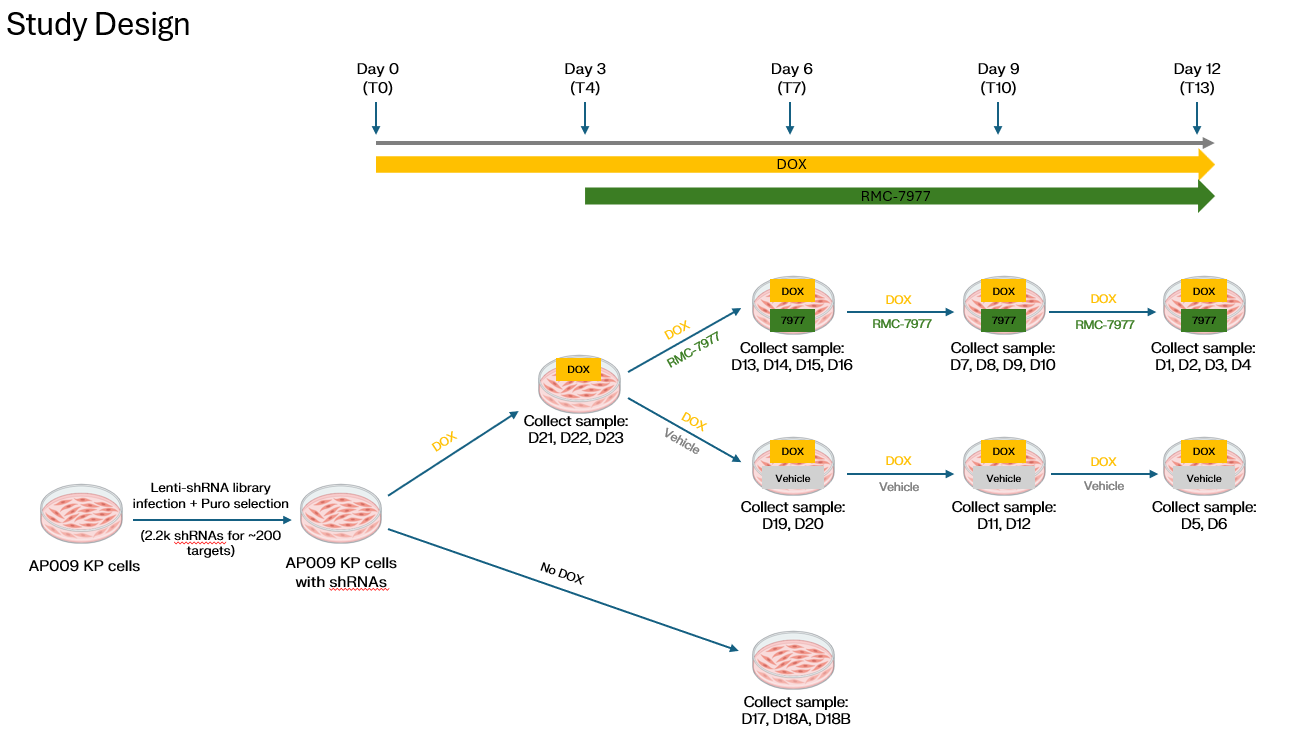
\includegraphics[keepaspectratio]{schematic_workflow_experimental_design.png}}
\caption{multiplexed shRNA screening experiment}
\end{figure}

    \begin{tcolorbox}[breakable, size=fbox, boxrule=1pt, pad at break*=1mm,colback=cellbackground, colframe=cellborder]
\prompt{In}{incolor}{5}{\boxspacing}
\begin{Verbatim}[commandchars=\\\{\}]
\PY{c+c1}{\PYZsh{} \PYZsh{}\PYZsh{}\PYZsh{}\PYZsh{} experimental design xlsx file}
\PY{c+c1}{\PYZsh{} file\PYZus{}path = \PYZdq{}\PYZti{}/Documents/Projects/Multi\PYZus{}shRNA\PYZus{}screening\PYZus{}AP009/data/Multiplexed shRNA screen in 2D AP009 \PYZhy{} Cellecta.xlsx\PYZdq{}}

\PY{c+c1}{\PYZsh{} xls = pd.ExcelFile(file\PYZus{}path)}

\PY{c+c1}{\PYZsh{} \PYZsh{}\PYZsh{} Gene targets}
\PY{c+c1}{\PYZsh{} gene\PYZus{}targets\PYZus{}df = pd.read\PYZus{}excel(xls, sheet\PYZus{}name=\PYZdq{}Master list\PYZdq{})}
\PY{c+c1}{\PYZsh{} \PYZsh{} Filter out \PYZdq{}Individual dual shRNA vector\PYZdq{} from gene targets}
\PY{c+c1}{\PYZsh{} filtered\PYZus{}gene\PYZus{}targets\PYZus{}df = gene\PYZus{}targets\PYZus{}df[gene\PYZus{}targets\PYZus{}df[\PYZdq{}Vector type\PYZdq{}] != \PYZdq{}Individual dual shRNA vector\PYZdq{}]}
\PY{c+c1}{\PYZsh{} filtered\PYZus{}gene\PYZus{}targets = filtered\PYZus{}gene\PYZus{}targets\PYZus{}df[\PYZdq{}Mouse gene symbol\PYZdq{}].dropna().unique()}

\PY{c+c1}{\PYZsh{} \PYZsh{} \PYZsh{}\PYZsh{} Define experimental parameters}
\PY{c+c1}{\PYZsh{} \PYZsh{} \PYZsh{} Num clonal barcodes per gene}
\PY{c+c1}{\PYZsh{} \PYZsh{} num\PYZus{}clonal\PYZus{}barcodes = 12000  }
\PY{c+c1}{\PYZsh{} \PYZsh{} \PYZsh{} Num shRNAs per gene}
\PY{c+c1}{\PYZsh{} \PYZsh{} num\PYZus{}shRNAs\PYZus{}per\PYZus{}gene = 10  }
\PY{c+c1}{\PYZsh{} \PYZsh{} \PYZsh{} N\PYZus{}reps per condition per timepoint}
\PY{c+c1}{\PYZsh{} \PYZsh{} num\PYZus{}replicates = 2  }

\PY{c+c1}{\PYZsh{} \PYZsh{}\PYZsh{} Define experimental conditions and timepoints }
\PY{c+c1}{\PYZsh{} \PYZsh{} available timepoints}
\PY{c+c1}{\PYZsh{} time\PYZus{}points = [\PYZdq{}0d\PYZdq{}, \PYZdq{}3d\PYZdq{}, \PYZdq{}6d\PYZdq{}, \PYZdq{}9d\PYZdq{}]}
\PY{c+c1}{\PYZsh{} \PYZsh{} experimental conditions based on design}
\PY{c+c1}{\PYZsh{} conditions = [}
\PY{c+c1}{\PYZsh{}     \PYZdq{}Baseline\PYZus{}NoDox\PYZus{}Vehicle\PYZdq{},}
\PY{c+c1}{\PYZsh{}     \PYZdq{}Baseline\PYZus{}Dox\PYZus{}PreTx\PYZdq{},  \PYZsh{} Only at 0d}
\PY{c+c1}{\PYZsh{}     \PYZdq{}Prognostic\PYZus{}Dox\PYZus{}Vehicle\PYZdq{},}
\PY{c+c1}{\PYZsh{}     \PYZdq{}Predictive\PYZus{}Dox\PYZus{}7977\PYZus{}LowDose\PYZdq{},  \PYZsh{} IC30 early, IC50 later}
\PY{c+c1}{\PYZsh{}     \PYZdq{}Predictive\PYZus{}Dox\PYZus{}7977\PYZus{}HighDose\PYZdq{}  \PYZsh{} IC90}
\PY{c+c1}{\PYZsh{} ]}
\end{Verbatim}
\end{tcolorbox}

    \begin{tcolorbox}[breakable, size=fbox, boxrule=1pt, pad at break*=1mm,colback=cellbackground, colframe=cellborder]
\prompt{In}{incolor}{6}{\boxspacing}
\begin{Verbatim}[commandchars=\\\{\}]
\PY{c+c1}{\PYZsh{}\PYZsh{}\PYZsh{}\PYZsh{} sample description xlsx file}
\PY{n}{file\PYZus{}path\PYZus{}cellecta} \PY{o}{=} \PY{l+s+s2}{\PYZdq{}}\PY{l+s+s2}{\PYZti{}/Documents/Projects/Multi\PYZus{}shRNA\PYZus{}screening\PYZus{}AP009/data/sample\PYZus{}description\PYZus{}rectified.xlsx}\PY{l+s+s2}{\PYZdq{}}

\PY{n}{df\PYZus{}sd} \PY{o}{=} \PY{n}{pd}\PY{o}{.}\PY{n}{read\PYZus{}excel}\PY{p}{(}\PY{n}{file\PYZus{}path\PYZus{}cellecta}\PY{p}{,} \PY{n}{sheet\PYZus{}name}\PY{o}{=}\PY{l+s+s1}{\PYZsq{}}\PY{l+s+s1}{Sheet1}\PY{l+s+s1}{\PYZsq{}}\PY{p}{)}

\PY{c+c1}{\PYZsh{} Set the first row as column headers and remove it from the data}
\PY{n}{df\PYZus{}sd}\PY{o}{.}\PY{n}{columns} \PY{o}{=} \PY{n}{df\PYZus{}sd}\PY{o}{.}\PY{n}{iloc}\PY{p}{[}\PY{l+m+mi}{0}\PY{p}{]}
\PY{n}{df\PYZus{}sd} \PY{o}{=} \PY{n}{df\PYZus{}sd}\PY{p}{[}\PY{l+m+mi}{1}\PY{p}{:}\PY{p}{]}\PY{o}{.}\PY{n}{reset\PYZus{}index}\PY{p}{(}\PY{n}{drop}\PY{o}{=}\PY{k+kc}{True}\PY{p}{)}

\PY{c+c1}{\PYZsh{} Rename columns to remove any unintended whitespace}
\PY{n}{df\PYZus{}sd}\PY{o}{.}\PY{n}{columns} \PY{o}{=} \PY{n}{df\PYZus{}sd}\PY{o}{.}\PY{n}{columns}\PY{o}{.}\PY{n}{str}\PY{o}{.}\PY{n}{strip}\PY{p}{(}\PY{p}{)}
\end{Verbatim}
\end{tcolorbox}

    Utility function of table viewing

    \begin{tcolorbox}[breakable, size=fbox, boxrule=1pt, pad at break*=1mm,colback=cellbackground, colframe=cellborder]
\prompt{In}{incolor}{7}{\boxspacing}
\begin{Verbatim}[commandchars=\\\{\}]
\PY{c+c1}{\PYZsh{}\PYZsh{} utility function of printing table}
\PY{k}{def} \PY{n+nf}{ViewTable}\PY{p}{(}\PY{n}{df}\PY{p}{,} \PY{n}{top\PYZus{}n\PYZus{}rows} \PY{o}{=} \PY{k+kc}{None}\PY{p}{)}\PY{p}{:}
    \PY{n}{table} \PY{o}{=} \PY{n}{PrettyTable}\PY{p}{(}\PY{n}{df}\PY{o}{.}\PY{n}{columns}\PY{o}{.}\PY{n}{tolist}\PY{p}{(}\PY{p}{)}\PY{p}{)}
    \PY{k}{if} \PY{n}{top\PYZus{}n\PYZus{}rows}\PY{p}{:}
        \PY{n}{df\PYZus{}tmp} \PY{o}{=} \PY{n}{df}\PY{o}{.}\PY{n}{head}\PY{p}{(}\PY{n}{top\PYZus{}n\PYZus{}rows}\PY{p}{)}
    \PY{k}{else}\PY{p}{:}
        \PY{n}{df\PYZus{}tmp} \PY{o}{=} \PY{n}{df}
    \PY{k}{for} \PY{n}{row} \PY{o+ow}{in} \PY{n}{df\PYZus{}tmp}\PY{o}{.}\PY{n}{itertuples}\PY{p}{(}\PY{n}{index}\PY{o}{=}\PY{k+kc}{False}\PY{p}{,} \PY{n}{name}\PY{o}{=}\PY{k+kc}{None}\PY{p}{)}\PY{p}{:}
        \PY{n}{table}\PY{o}{.}\PY{n}{add\PYZus{}row}\PY{p}{(}\PY{n}{row}\PY{p}{)}
    \PY{n+nb}{print}\PY{p}{(}\PY{n}{table}\PY{p}{)}

\PY{n}{ViewTable}\PY{p}{(}\PY{n}{df\PYZus{}sd}\PY{p}{,} \PY{l+m+mi}{5}\PY{p}{)}
\end{Verbatim}
\end{tcolorbox}

    \begin{Verbatim}[commandchars=\\\{\}]
+-----------+--------------------+----------------+-----------------------------
-------------------+-------------------+---------+-------+--------+-----------+-
----+------+
| Sample\_ID | Sample\_Description |    Library     |                     Vector
|      Flowcell     |    Tx   | Group | Day\_Tx | Replicate | Dox | Note |
+-----------+--------------------+----------------+-----------------------------
-------------------+-------------------+---------+-------+--------+-----------+-
----+------+
|     D1    |   T13\_Dox\_0.6nM    | 2.2K-REVMED-ZZ |  pRSIT16cb-U6tet-sh-CMV-
tetR-2A-TagRFP-2A-Puro | 25-03-11  102190  |   Low   |   5   |   9    |     2
|  Y  | nan  |
|     D2    |   T13\_Dox\_0.6nM    | 2.2K-REVMED-ZZ |  pRSIT16cb-U6tet-sh-CMV-
tetR-2A-TagRFP-2A-Puro | 25-03-11  102190  |   Low   |   5   |   9    |     1
|  Y  | nan  |
|     D3    |   T13\_Dox\_3.5nM    | 2.2K-REVMED-ZZ |  pRSIT16cb-U6tet-sh-CMV-
tetR-2A-TagRFP-2A-Puro | 25-03-11  102190  |   High  |   4   |   9    |     2
|  Y  | nan  |
|     D4    |   T13\_Dox\_3.5nM    | 2.2K-REVMED-ZZ |  pRSIT16cb-U6tet-sh-CMV-
tetR-2A-TagRFP-2A-Puro | 25-03-11  102190  |   High  |   4   |   9    |     1
|  Y  | nan  |
|     D5    |  T13\_Dox\_Vehicle   | 2.2K-REVMED-ZZ |  pRSIT16cb-U6tet-sh-CMV-
tetR-2A-TagRFP-2A-Puro | 25-03-11  102190  | Vehicle |   2   |   9    |     2
|  Y  | nan  |
+-----------+--------------------+----------------+-----------------------------
-------------------+-------------------+---------+-------+--------+-----------+-
----+------+
    \end{Verbatim}

    \subsection{Barcodes (shRNA) count
table}\label{barcodes-shrna-count-table}

Load count table (from Cellecta) and extract fields of sample IDs and
target gene

    \begin{tcolorbox}[breakable, size=fbox, boxrule=1pt, pad at break*=1mm,colback=cellbackground, colframe=cellborder]
\prompt{In}{incolor}{8}{\boxspacing}
\begin{Verbatim}[commandchars=\\\{\}]
\PY{n}{file\PYZus{}path\PYZus{}count\PYZus{}table} \PY{o}{=} \PY{l+s+s2}{\PYZdq{}}\PY{l+s+s2}{\PYZti{}/Documents/Projects/Multi\PYZus{}shRNA\PYZus{}screening\PYZus{}AP009/data/Count\PYZus{}Table.csv}\PY{l+s+s2}{\PYZdq{}}
\PY{n}{df\PYZus{}counts} \PY{o}{=} \PY{n}{pd}\PY{o}{.}\PY{n}{read\PYZus{}csv}\PY{p}{(}\PY{n}{file\PYZus{}path\PYZus{}count\PYZus{}table}\PY{p}{)}

\PY{c+c1}{\PYZsh{} Extract columns that start with \PYZsq{}D\PYZsq{} plus the \PYZsq{}Gene Symbol / Target Name\PYZsq{} column}
\PY{n}{selected\PYZus{}columns} \PY{o}{=} \PY{p}{[}\PY{n}{col} \PY{k}{for} \PY{n}{col} \PY{o+ow}{in} \PY{n}{df\PYZus{}counts}\PY{o}{.}\PY{n}{columns} \PY{k}{if} \PY{n}{col}\PY{o}{.}\PY{n}{startswith}\PY{p}{(}\PY{l+s+s2}{\PYZdq{}}\PY{l+s+s2}{D}\PY{l+s+s2}{\PYZdq{}}\PY{p}{)}\PY{p}{]} \PY{o}{+} \PY{p}{[}\PY{l+s+s2}{\PYZdq{}}\PY{l+s+s2}{Gene Symbol / Target Name}\PY{l+s+s2}{\PYZdq{}}\PY{p}{]}

\PY{c+c1}{\PYZsh{} Create a new dataframe with selected columns}
\PY{n}{df\PYZus{}counts} \PY{o}{=} \PY{n}{df\PYZus{}counts}\PY{p}{[}\PY{n}{selected\PYZus{}columns}\PY{p}{]}\PY{o}{.}\PY{n}{copy}\PY{p}{(}\PY{p}{)}

\PY{c+c1}{\PYZsh{} Rename \PYZsq{}Gene Symbol / Target Name\PYZsq{} to \PYZsq{}target\PYZus{}gene\PYZsq{}}
\PY{n}{df\PYZus{}counts} \PY{o}{=} \PY{n}{df\PYZus{}counts}\PY{o}{.}\PY{n}{rename}\PY{p}{(}\PY{n}{columns}\PY{o}{=}\PY{p}{\PYZob{}}\PY{l+s+s2}{\PYZdq{}}\PY{l+s+s2}{Gene Symbol / Target Name}\PY{l+s+s2}{\PYZdq{}}\PY{p}{:} \PY{l+s+s2}{\PYZdq{}}\PY{l+s+s2}{Target\PYZus{}Gene}\PY{l+s+s2}{\PYZdq{}}\PY{p}{\PYZcb{}}\PY{p}{)}

\PY{c+c1}{\PYZsh{} Rename \PYZsq{}Non\PYZhy{}Targeting\PYZhy{}Mouse\PYZsq{} to \PYZsq{}NT\PYZsq{} in the target\PYZus{}gene column}
\PY{n}{df\PYZus{}counts}\PY{p}{[}\PY{l+s+s2}{\PYZdq{}}\PY{l+s+s2}{Target\PYZus{}Gene}\PY{l+s+s2}{\PYZdq{}}\PY{p}{]} \PY{o}{=} \PY{n}{df\PYZus{}counts}\PY{p}{[}\PY{l+s+s2}{\PYZdq{}}\PY{l+s+s2}{Target\PYZus{}Gene}\PY{l+s+s2}{\PYZdq{}}\PY{p}{]}\PY{o}{.}\PY{n}{replace}\PY{p}{(}\PY{l+s+s2}{\PYZdq{}}\PY{l+s+s2}{Non\PYZhy{}Targeting\PYZhy{}Mouse}\PY{l+s+s2}{\PYZdq{}}\PY{p}{,} \PY{l+s+s2}{\PYZdq{}}\PY{l+s+s2}{NT}\PY{l+s+s2}{\PYZdq{}}\PY{p}{)}

\PY{c+c1}{\PYZsh{} Ensure there are no NaN values in the target\PYZus{}gene column before counting repeats}
\PY{n}{df\PYZus{}counts}\PY{p}{[}\PY{l+s+s2}{\PYZdq{}}\PY{l+s+s2}{Target\PYZus{}Gene}\PY{l+s+s2}{\PYZdq{}}\PY{p}{]} \PY{o}{=} \PY{n}{df\PYZus{}counts}\PY{p}{[}\PY{l+s+s2}{\PYZdq{}}\PY{l+s+s2}{Target\PYZus{}Gene}\PY{l+s+s2}{\PYZdq{}}\PY{p}{]}\PY{o}{.}\PY{n}{fillna}\PY{p}{(}\PY{l+s+s2}{\PYZdq{}}\PY{l+s+s2}{Unknown}\PY{l+s+s2}{\PYZdq{}}\PY{p}{)}

\PY{c+c1}{\PYZsh{} Generate a sequential ID for each occurrence of target\PYZus{}gene}
\PY{n}{df\PYZus{}counts}\PY{p}{[}\PY{l+s+s2}{\PYZdq{}}\PY{l+s+s2}{target\PYZus{}gene\PYZus{}repeat\PYZus{}ID}\PY{l+s+s2}{\PYZdq{}}\PY{p}{]} \PY{o}{=} \PY{n}{df\PYZus{}counts}\PY{o}{.}\PY{n}{groupby}\PY{p}{(}\PY{l+s+s2}{\PYZdq{}}\PY{l+s+s2}{Target\PYZus{}Gene}\PY{l+s+s2}{\PYZdq{}}\PY{p}{)}\PY{o}{.}\PY{n}{cumcount}\PY{p}{(}\PY{p}{)} \PY{o}{+} \PY{l+m+mi}{1}

\PY{c+c1}{\PYZsh{} Format as \PYZdq{}01\PYZdq{}, \PYZdq{}02\PYZdq{}, \PYZdq{}03\PYZdq{}, etc.}
\PY{n}{df\PYZus{}counts}\PY{p}{[}\PY{l+s+s2}{\PYZdq{}}\PY{l+s+s2}{target\PYZus{}gene\PYZus{}repeat\PYZus{}ID}\PY{l+s+s2}{\PYZdq{}}\PY{p}{]} \PY{o}{=} \PY{n}{df\PYZus{}counts}\PY{p}{[}\PY{l+s+s2}{\PYZdq{}}\PY{l+s+s2}{target\PYZus{}gene\PYZus{}repeat\PYZus{}ID}\PY{l+s+s2}{\PYZdq{}}\PY{p}{]}\PY{o}{.}\PY{n}{astype}\PY{p}{(}\PY{n+nb}{int}\PY{p}{)}\PY{o}{.}\PY{n}{apply}\PY{p}{(}\PY{k}{lambda} \PY{n}{x}\PY{p}{:} \PY{l+s+sa}{f}\PY{l+s+s2}{\PYZdq{}}\PY{l+s+si}{\PYZob{}}\PY{n}{x}\PY{l+s+si}{:}\PY{l+s+s2}{02d}\PY{l+s+si}{\PYZcb{}}\PY{l+s+s2}{\PYZdq{}}\PY{p}{)}

\PY{c+c1}{\PYZsh{} Combine with target\PYZus{}gene to create a unique ID}
\PY{n}{df\PYZus{}counts}\PY{p}{[}\PY{l+s+s2}{\PYZdq{}}\PY{l+s+s2}{shRNA\PYZus{}ID}\PY{l+s+s2}{\PYZdq{}}\PY{p}{]} \PY{o}{=} \PY{n}{df\PYZus{}counts}\PY{p}{[}\PY{l+s+s2}{\PYZdq{}}\PY{l+s+s2}{Target\PYZus{}Gene}\PY{l+s+s2}{\PYZdq{}}\PY{p}{]} \PY{o}{+} \PY{l+s+s2}{\PYZdq{}}\PY{l+s+s2}{\PYZus{}}\PY{l+s+s2}{\PYZdq{}} \PY{o}{+} \PY{n}{df\PYZus{}counts}\PY{p}{[}\PY{l+s+s2}{\PYZdq{}}\PY{l+s+s2}{target\PYZus{}gene\PYZus{}repeat\PYZus{}ID}\PY{l+s+s2}{\PYZdq{}}\PY{p}{]}

\PY{c+c1}{\PYZsh{} Drop the temporary repeat ID column}
\PY{n}{df\PYZus{}counts} \PY{o}{=} \PY{n}{df\PYZus{}counts}\PY{o}{.}\PY{n}{drop}\PY{p}{(}\PY{n}{columns}\PY{o}{=}\PY{p}{[}\PY{l+s+s2}{\PYZdq{}}\PY{l+s+s2}{target\PYZus{}gene\PYZus{}repeat\PYZus{}ID}\PY{l+s+s2}{\PYZdq{}}\PY{p}{]}\PY{p}{)}

\PY{c+c1}{\PYZsh{} Update the target\PYZus{}gene\PYZus{}ID column accordingly}
\PY{n}{df\PYZus{}counts}\PY{p}{[}\PY{l+s+s2}{\PYZdq{}}\PY{l+s+s2}{shRNA\PYZus{}ID}\PY{l+s+s2}{\PYZdq{}}\PY{p}{]} \PY{o}{=} \PY{n}{df\PYZus{}counts}\PY{p}{[}\PY{l+s+s2}{\PYZdq{}}\PY{l+s+s2}{Target\PYZus{}Gene}\PY{l+s+s2}{\PYZdq{}}\PY{p}{]} \PY{o}{+} \PY{l+s+s2}{\PYZdq{}}\PY{l+s+s2}{\PYZus{}}\PY{l+s+s2}{\PYZdq{}} \PY{o}{+} \PY{n}{df\PYZus{}counts}\PY{p}{[}\PY{l+s+s2}{\PYZdq{}}\PY{l+s+s2}{shRNA\PYZus{}ID}\PY{l+s+s2}{\PYZdq{}}\PY{p}{]}\PY{o}{.}\PY{n}{str}\PY{o}{.}\PY{n}{split}\PY{p}{(}\PY{l+s+s2}{\PYZdq{}}\PY{l+s+s2}{\PYZus{}}\PY{l+s+s2}{\PYZdq{}}\PY{p}{)}\PY{o}{.}\PY{n}{str}\PY{p}{[}\PY{o}{\PYZhy{}}\PY{l+m+mi}{1}\PY{p}{]}

\PY{c+c1}{\PYZsh{} melt the dataframe to long format }
\PY{n}{df\PYZus{}long} \PY{o}{=} \PY{n}{df\PYZus{}counts}\PY{o}{.}\PY{n}{melt}\PY{p}{(}\PY{n}{id\PYZus{}vars}\PY{o}{=}\PY{p}{[}\PY{l+s+s2}{\PYZdq{}}\PY{l+s+s2}{Target\PYZus{}Gene}\PY{l+s+s2}{\PYZdq{}}\PY{p}{,} \PY{l+s+s2}{\PYZdq{}}\PY{l+s+s2}{shRNA\PYZus{}ID}\PY{l+s+s2}{\PYZdq{}}\PY{p}{]}\PY{p}{,} \PY{n}{var\PYZus{}name}\PY{o}{=}\PY{l+s+s2}{\PYZdq{}}\PY{l+s+s2}{Sample\PYZus{}ID}\PY{l+s+s2}{\PYZdq{}}\PY{p}{,} \PY{n}{value\PYZus{}name}\PY{o}{=}\PY{l+s+s2}{\PYZdq{}}\PY{l+s+s2}{Read\PYZus{}Counts}\PY{l+s+s2}{\PYZdq{}}\PY{p}{)}
\end{Verbatim}
\end{tcolorbox}

    \begin{tcolorbox}[breakable, size=fbox, boxrule=1pt, pad at break*=1mm,colback=cellbackground, colframe=cellborder]
\prompt{In}{incolor}{9}{\boxspacing}
\begin{Verbatim}[commandchars=\\\{\}]
\PY{n}{display}\PY{p}{(}\PY{n}{df\PYZus{}counts}\PY{p}{)}
\end{Verbatim}
\end{tcolorbox}

    
    \begin{Verbatim}[commandchars=\\\{\}]
        D1    D2    D3    D4    D5    D6    D7    D8    D9   D10  {\ldots}   D17  \textbackslash{}
0     1399  2777  1312  2281  2056  1579  1072  3116  2532  3019  {\ldots}  1683   
1     1785  3277  1776  3414  3139  2482  1289  3877  3373  3953  {\ldots}  2239   
2      569  1270   539  1025  1075   892   484  1728  1201  1301  {\ldots}   727   
3      955  1703   912  1607  1714  1235   817  2199  1727  2160  {\ldots}  1234   
4     1150  2403  1177  2281  1981  1467  1055  2641  2071  2504  {\ldots}  1462   
{\ldots}    {\ldots}   {\ldots}   {\ldots}   {\ldots}   {\ldots}   {\ldots}   {\ldots}   {\ldots}   {\ldots}   {\ldots}  {\ldots}   {\ldots}   
2182   460   889   548   870   810   571   332  1141   935  1101  {\ldots}   723   
2183   725  1451   709  1416  1151  1017   483  1693  1601  1726  {\ldots}   936   
2184   547  1133   575  1052  1093   843   477  1365  1246  1497  {\ldots}   777   
2185  1354  2584  1371  2570  2230  1773  1047  3223  2530  3248  {\ldots}  1740   
2186   479   960   497   907   832   562   368  1276   813  1025  {\ldots}   593   

      D18-A  D18-B   D19   D20   D21   D22   D23  Target\_Gene  shRNA\_ID  
0      1411   1717  1682  2105  1482  1257  1965           NT     NT\_01  
1      2000   2510  2559  2959  2321  1782  2763           NT     NT\_02  
2       726    804   774  1094   768   601   945           NT     NT\_03  
3      1153   1372  1268  1481  1010   855  1385           NT     NT\_04  
4      1415   1599  1556  2025  1541  1126  1868           NT     NT\_05  
{\ldots}     {\ldots}    {\ldots}   {\ldots}   {\ldots}   {\ldots}   {\ldots}   {\ldots}          {\ldots}       {\ldots}  
2182    679    758   709   892   658   475   859         Zeb1   Zeb1\_06  
2183    782    970   933  1242   931   757  1071         Zeb1   Zeb1\_07  
2184    771    868   820  1157   698   637   846         Zeb1   Zeb1\_08  
2185   1610   1877  1745  2160  1681  1329  1973         Zeb1   Zeb1\_09  
2186    534    597   583   787   609   474   691         Zeb1   Zeb1\_10  

[2187 rows x 26 columns]
    \end{Verbatim}

    
    \begin{tcolorbox}[breakable, size=fbox, boxrule=1pt, pad at break*=1mm,colback=cellbackground, colframe=cellborder]
\prompt{In}{incolor}{10}{\boxspacing}
\begin{Verbatim}[commandchars=\\\{\}]
\PY{n}{display}\PY{p}{(}\PY{n}{df\PYZus{}long}\PY{p}{)}
\end{Verbatim}
\end{tcolorbox}

    
    \begin{Verbatim}[commandchars=\\\{\}]
      Target\_Gene shRNA\_ID Sample\_ID  Read\_Counts
0              NT    NT\_01        D1         1399
1              NT    NT\_02        D1         1785
2              NT    NT\_03        D1          569
3              NT    NT\_04        D1          955
4              NT    NT\_05        D1         1150
{\ldots}           {\ldots}      {\ldots}       {\ldots}          {\ldots}
52483        Zeb1  Zeb1\_06       D23          859
52484        Zeb1  Zeb1\_07       D23         1071
52485        Zeb1  Zeb1\_08       D23          846
52486        Zeb1  Zeb1\_09       D23         1973
52487        Zeb1  Zeb1\_10       D23          691

[52488 rows x 4 columns]
    \end{Verbatim}

    
    \begin{tcolorbox}[breakable, size=fbox, boxrule=1pt, pad at break*=1mm,colback=cellbackground, colframe=cellborder]
\prompt{In}{incolor}{11}{\boxspacing}
\begin{Verbatim}[commandchars=\\\{\}]
\PY{c+c1}{\PYZsh{}\PYZsh{}\PYZsh{} total number of barcodes per sample / condition}
\end{Verbatim}
\end{tcolorbox}

    \begin{tcolorbox}[breakable, size=fbox, boxrule=1pt, pad at break*=1mm,colback=cellbackground, colframe=cellborder]
\prompt{In}{incolor}{12}{\boxspacing}
\begin{Verbatim}[commandchars=\\\{\}]
\PY{n}{df\PYZus{}full} \PY{o}{=} \PY{n}{df\PYZus{}long}\PY{o}{.}\PY{n}{merge}\PY{p}{(}\PY{n}{df\PYZus{}sd}\PY{p}{[}\PY{p}{[}\PY{l+s+s2}{\PYZdq{}}\PY{l+s+s2}{Sample\PYZus{}ID}\PY{l+s+s2}{\PYZdq{}}\PY{p}{,} \PY{l+s+s2}{\PYZdq{}}\PY{l+s+s2}{Sample\PYZus{}Description}\PY{l+s+s2}{\PYZdq{}}\PY{p}{,} \PY{l+s+s2}{\PYZdq{}}\PY{l+s+s2}{Day\PYZus{}Tx}\PY{l+s+s2}{\PYZdq{}}\PY{p}{,} \PY{l+s+s2}{\PYZdq{}}\PY{l+s+s2}{Tx}\PY{l+s+s2}{\PYZdq{}}\PY{p}{,} \PY{l+s+s2}{\PYZdq{}}\PY{l+s+s2}{Dox}\PY{l+s+s2}{\PYZdq{}}\PY{p}{,} \PY{l+s+s2}{\PYZdq{}}\PY{l+s+s2}{Replicate}\PY{l+s+s2}{\PYZdq{}}\PY{p}{]}\PY{p}{]}\PY{p}{,} 
                        \PY{n}{left\PYZus{}on} \PY{o}{=} \PY{l+s+s2}{\PYZdq{}}\PY{l+s+s2}{Sample\PYZus{}ID}\PY{l+s+s2}{\PYZdq{}}\PY{p}{,} \PY{n}{right\PYZus{}on} \PY{o}{=} \PY{l+s+s2}{\PYZdq{}}\PY{l+s+s2}{Sample\PYZus{}ID}\PY{l+s+s2}{\PYZdq{}}\PY{p}{,} \PY{n}{how} \PY{o}{=} \PY{l+s+s2}{\PYZdq{}}\PY{l+s+s2}{left}\PY{l+s+s2}{\PYZdq{}}\PY{p}{)}
\PY{n}{df\PYZus{}full}\PY{o}{.}\PY{n}{to\PYZus{}csv}\PY{p}{(}\PY{l+s+s2}{\PYZdq{}}\PY{l+s+s2}{\PYZti{}/Documents/Projects/Multi\PYZus{}shRNA\PYZus{}screening\PYZus{}AP009/data/long\PYZus{}format\PYZus{}joint\PYZus{}count\PYZus{}data.csv}\PY{l+s+s2}{\PYZdq{}}\PY{p}{,} \PY{n}{index} \PY{o}{=} \PY{k+kc}{False}\PY{p}{)}
\end{Verbatim}
\end{tcolorbox}

    \begin{tcolorbox}[breakable, size=fbox, boxrule=1pt, pad at break*=1mm,colback=cellbackground, colframe=cellborder]
\prompt{In}{incolor}{13}{\boxspacing}
\begin{Verbatim}[commandchars=\\\{\}]
\PY{n}{display}\PY{p}{(}\PY{n}{df\PYZus{}full}\PY{p}{)}
\PY{n+nb}{print}\PY{p}{(}\PY{n}{df\PYZus{}full}\PY{p}{[}\PY{l+s+s2}{\PYZdq{}}\PY{l+s+s2}{Target\PYZus{}Gene}\PY{l+s+s2}{\PYZdq{}}\PY{p}{]}\PY{o}{.}\PY{n}{value\PYZus{}counts}\PY{p}{(}\PY{p}{)}\PY{p}{)}
\end{Verbatim}
\end{tcolorbox}

    
    \begin{Verbatim}[commandchars=\\\{\}]
      Target\_Gene shRNA\_ID Sample\_ID  Read\_Counts Sample\_Description Day\_Tx  \textbackslash{}
0              NT    NT\_01        D1         1399      T13\_Dox\_0.6nM      9   
1              NT    NT\_02        D1         1785      T13\_Dox\_0.6nM      9   
2              NT    NT\_03        D1          569      T13\_Dox\_0.6nM      9   
3              NT    NT\_04        D1          955      T13\_Dox\_0.6nM      9   
4              NT    NT\_05        D1         1150      T13\_Dox\_0.6nM      9   
{\ldots}           {\ldots}      {\ldots}       {\ldots}          {\ldots}                {\ldots}    {\ldots}   
52483        Zeb1  Zeb1\_06       D23          859        T4\_Dox\_NoTx      0   
52484        Zeb1  Zeb1\_07       D23         1071        T4\_Dox\_NoTx      0   
52485        Zeb1  Zeb1\_08       D23          846        T4\_Dox\_NoTx      0   
52486        Zeb1  Zeb1\_09       D23         1973        T4\_Dox\_NoTx      0   
52487        Zeb1  Zeb1\_10       D23          691        T4\_Dox\_NoTx      0   

         Tx Dox Replicate  
0       Low   Y         2  
1       Low   Y         2  
2       Low   Y         2  
3       Low   Y         2  
4       Low   Y         2  
{\ldots}     {\ldots}  ..       {\ldots}  
52483  None   Y         1  
52484  None   Y         1  
52485  None   Y         1  
52486  None   Y         1  
52487  None   Y         1  

[52488 rows x 9 columns]
    \end{Verbatim}

    
    \begin{Verbatim}[commandchars=\\\{\}]
NT               4800
Pdgfra            240
Nf1               240
Nf2               240
Nfe2l2            240
                 {\ldots}
Erbb2             240
Erbb3             240
Ern1              240
Zeb1              240
Cdkn2a(Ink4a)     168
Name: Target\_Gene, Length: 200, dtype: int64
    \end{Verbatim}

    Plot total read counts per sample

    \begin{tcolorbox}[breakable, size=fbox, boxrule=1pt, pad at break*=1mm,colback=cellbackground, colframe=cellborder]
\prompt{In}{incolor}{14}{\boxspacing}
\begin{Verbatim}[commandchars=\\\{\}]
\PY{c+c1}{\PYZsh{} Aggregate total read counts per sample}
\PY{n}{df\PYZus{}sample\PYZus{}counts\PYZus{}simple} \PY{o}{=} \PY{n}{df\PYZus{}full}\PY{o}{.}\PY{n}{groupby}\PY{p}{(}\PY{p}{[}\PY{l+s+s2}{\PYZdq{}}\PY{l+s+s2}{Sample\PYZus{}ID}\PY{l+s+s2}{\PYZdq{}}\PY{p}{,} \PY{l+s+s2}{\PYZdq{}}\PY{l+s+s2}{Sample\PYZus{}Description}\PY{l+s+s2}{\PYZdq{}}\PY{p}{]}\PY{p}{)}\PY{p}{[}\PY{l+s+s2}{\PYZdq{}}\PY{l+s+s2}{Read\PYZus{}Counts}\PY{l+s+s2}{\PYZdq{}}\PY{p}{]}\PY{o}{.}\PY{n}{sum}\PY{p}{(}\PY{p}{)}\PY{o}{.}\PY{n}{reset\PYZus{}index}\PY{p}{(}\PY{p}{)}

\PY{c+c1}{\PYZsh{} Ensure Sample\PYZus{}ID is sorted numerically rather than lexicographically}
\PY{n}{df\PYZus{}sample\PYZus{}counts\PYZus{}simple}\PY{p}{[}\PY{l+s+s2}{\PYZdq{}}\PY{l+s+s2}{Sample\PYZus{}ID\PYZus{}Sort}\PY{l+s+s2}{\PYZdq{}}\PY{p}{]} \PY{o}{=} \PY{n}{df\PYZus{}sample\PYZus{}counts\PYZus{}simple}\PY{p}{[}\PY{l+s+s2}{\PYZdq{}}\PY{l+s+s2}{Sample\PYZus{}ID}\PY{l+s+s2}{\PYZdq{}}\PY{p}{]}\PY{o}{.}\PY{n}{str}\PY{o}{.}\PY{n}{extract}\PY{p}{(}\PY{l+s+s1}{\PYZsq{}}\PY{l+s+s1}{(}\PY{l+s+s1}{\PYZbs{}}\PY{l+s+s1}{d+)}\PY{l+s+s1}{\PYZsq{}}\PY{p}{)}\PY{o}{.}\PY{n}{astype}\PY{p}{(}\PY{n+nb}{int}\PY{p}{)}
\PY{n}{df\PYZus{}sample\PYZus{}counts\PYZus{}simple} \PY{o}{=} \PY{n}{df\PYZus{}sample\PYZus{}counts\PYZus{}simple}\PY{o}{.}\PY{n}{sort\PYZus{}values}\PY{p}{(}\PY{n}{by}\PY{o}{=}\PY{l+s+s2}{\PYZdq{}}\PY{l+s+s2}{Sample\PYZus{}ID\PYZus{}Sort}\PY{l+s+s2}{\PYZdq{}}\PY{p}{)}\PY{o}{.}\PY{n}{reset\PYZus{}index}\PY{p}{(}\PY{p}{)}

\PY{c+c1}{\PYZsh{} Modify Sample\PYZus{}ID labels to include total counts in parentheses}
\PY{n}{df\PYZus{}sample\PYZus{}counts\PYZus{}simple}\PY{p}{[}\PY{l+s+s2}{\PYZdq{}}\PY{l+s+s2}{Sample\PYZus{}ID\PYZus{}Label}\PY{l+s+s2}{\PYZdq{}}\PY{p}{]} \PY{o}{=} \PY{n}{df\PYZus{}sample\PYZus{}counts\PYZus{}simple}\PY{o}{.}\PY{n}{apply}\PY{p}{(}
    \PY{k}{lambda} \PY{n}{row}\PY{p}{:} \PY{l+s+sa}{f}\PY{l+s+s2}{\PYZdq{}}\PY{l+s+si}{\PYZob{}}\PY{n}{row}\PY{p}{[}\PY{l+s+s1}{\PYZsq{}}\PY{l+s+s1}{Sample\PYZus{}ID}\PY{l+s+s1}{\PYZsq{}}\PY{p}{]}\PY{l+s+si}{\PYZcb{}}\PY{l+s+s2}{ (}\PY{l+s+si}{\PYZob{}}\PY{n+nb}{int}\PY{p}{(}\PY{n}{row}\PY{p}{[}\PY{l+s+s1}{\PYZsq{}}\PY{l+s+s1}{Read\PYZus{}Counts}\PY{l+s+s1}{\PYZsq{}}\PY{p}{]}\PY{p}{)}\PY{l+s+si}{\PYZcb{}}\PY{l+s+s2}{)}\PY{l+s+s2}{\PYZdq{}}\PY{p}{,} \PY{n}{axis}\PY{o}{=}\PY{l+m+mi}{1}
\PY{p}{)}

\PY{c+c1}{\PYZsh{} Plot the bar chart with modified x\PYZhy{}axis labels}
\PY{n}{plt}\PY{o}{.}\PY{n}{figure}\PY{p}{(}\PY{n}{figsize}\PY{o}{=}\PY{p}{(}\PY{l+m+mi}{12}\PY{p}{,} \PY{l+m+mi}{6}\PY{p}{)}\PY{p}{)}
\PY{n}{ax} \PY{o}{=} \PY{n}{sns}\PY{o}{.}\PY{n}{barplot}\PY{p}{(}\PY{n}{data}\PY{o}{=}\PY{n}{df\PYZus{}sample\PYZus{}counts\PYZus{}simple}\PY{p}{,} \PY{n}{x}\PY{o}{=}\PY{l+s+s2}{\PYZdq{}}\PY{l+s+s2}{Sample\PYZus{}ID\PYZus{}Label}\PY{l+s+s2}{\PYZdq{}}\PY{p}{,} \PY{n}{y}\PY{o}{=}\PY{l+s+s2}{\PYZdq{}}\PY{l+s+s2}{Read\PYZus{}Counts}\PY{l+s+s2}{\PYZdq{}}\PY{p}{,} \PY{n}{hue}\PY{o}{=}\PY{l+s+s2}{\PYZdq{}}\PY{l+s+s2}{Sample\PYZus{}Description}\PY{l+s+s2}{\PYZdq{}}\PY{p}{,} \PY{n}{dodge}\PY{o}{=}\PY{k+kc}{False}\PY{p}{)}

\PY{c+c1}{\PYZsh{} Identify group transitions for adding vertical dotted lines}
\PY{n}{prev\PYZus{}desc} \PY{o}{=} \PY{k+kc}{None}
\PY{k}{for} \PY{n}{index}\PY{p}{,} \PY{n}{row} \PY{o+ow}{in} \PY{n}{df\PYZus{}sample\PYZus{}counts\PYZus{}simple}\PY{o}{.}\PY{n}{iterrows}\PY{p}{(}\PY{p}{)}\PY{p}{:}
    \PY{n}{current\PYZus{}desc} \PY{o}{=} \PY{n}{row}\PY{p}{[}\PY{l+s+s2}{\PYZdq{}}\PY{l+s+s2}{Sample\PYZus{}Description}\PY{l+s+s2}{\PYZdq{}}\PY{p}{]}
    \PY{k}{if} \PY{n}{prev\PYZus{}desc} \PY{o+ow}{is} \PY{o+ow}{not} \PY{k+kc}{None} \PY{o+ow}{and} \PY{n}{prev\PYZus{}desc} \PY{o}{!=} \PY{n}{current\PYZus{}desc}\PY{p}{:}
        \PY{n}{plt}\PY{o}{.}\PY{n}{axvline}\PY{p}{(}\PY{n}{x}\PY{o}{=}\PY{n}{index} \PY{o}{\PYZhy{}} \PY{l+m+mf}{0.5}\PY{p}{,} \PY{n}{color}\PY{o}{=}\PY{l+s+s2}{\PYZdq{}}\PY{l+s+s2}{black}\PY{l+s+s2}{\PYZdq{}}\PY{p}{,} \PY{n}{linestyle}\PY{o}{=}\PY{l+s+s2}{\PYZdq{}}\PY{l+s+s2}{dotted}\PY{l+s+s2}{\PYZdq{}}\PY{p}{,} \PY{n}{linewidth}\PY{o}{=}\PY{l+m+mi}{1}\PY{p}{)}  \PY{c+c1}{\PYZsh{} Add vertical separator}
    \PY{n}{prev\PYZus{}desc} \PY{o}{=} \PY{n}{current\PYZus{}desc}

\PY{c+c1}{\PYZsh{} Set y\PYZhy{}axis to exact number format}
\PY{n}{plt}\PY{o}{.}\PY{n}{ticklabel\PYZus{}format}\PY{p}{(}\PY{n}{style}\PY{o}{=}\PY{l+s+s1}{\PYZsq{}}\PY{l+s+s1}{plain}\PY{l+s+s1}{\PYZsq{}}\PY{p}{,} \PY{n}{axis}\PY{o}{=}\PY{l+s+s1}{\PYZsq{}}\PY{l+s+s1}{y}\PY{l+s+s1}{\PYZsq{}}\PY{p}{)}  \PY{c+c1}{\PYZsh{} Disable scientific notation}

\PY{n}{plt}\PY{o}{.}\PY{n}{xticks}\PY{p}{(}\PY{n}{rotation}\PY{o}{=}\PY{l+m+mi}{90}\PY{p}{,} \PY{n}{fontsize}\PY{o}{=}\PY{l+m+mi}{8}\PY{p}{)}
\PY{n}{plt}\PY{o}{.}\PY{n}{xlabel}\PY{p}{(}\PY{l+s+s2}{\PYZdq{}}\PY{l+s+s2}{Sample ID (Total Read Counts)}\PY{l+s+s2}{\PYZdq{}}\PY{p}{)}
\PY{n}{plt}\PY{o}{.}\PY{n}{ylabel}\PY{p}{(}\PY{l+s+s2}{\PYZdq{}}\PY{l+s+s2}{Total Read Counts}\PY{l+s+s2}{\PYZdq{}}\PY{p}{)}
\PY{n}{plt}\PY{o}{.}\PY{n}{title}\PY{p}{(}\PY{l+s+s2}{\PYZdq{}}\PY{l+s+s2}{Total Read Counts per Sample (Ordered by Sample ID)}\PY{l+s+s2}{\PYZdq{}}\PY{p}{)}
\PY{n}{plt}\PY{o}{.}\PY{n}{legend}\PY{p}{(}\PY{n}{title}\PY{o}{=}\PY{l+s+s2}{\PYZdq{}}\PY{l+s+s2}{Sample Description}\PY{l+s+s2}{\PYZdq{}}\PY{p}{,} \PY{n}{bbox\PYZus{}to\PYZus{}anchor}\PY{o}{=}\PY{p}{(}\PY{l+m+mf}{1.05}\PY{p}{,} \PY{l+m+mi}{1}\PY{p}{)}\PY{p}{,} \PY{n}{loc}\PY{o}{=}\PY{l+s+s1}{\PYZsq{}}\PY{l+s+s1}{upper left}\PY{l+s+s1}{\PYZsq{}}\PY{p}{)}  \PY{c+c1}{\PYZsh{} Move legend outside}
\PY{n}{plt}\PY{o}{.}\PY{n}{show}\PY{p}{(}\PY{p}{)}
\end{Verbatim}
\end{tcolorbox}

    \begin{center}
    \adjustimage{max size={0.9\linewidth}{0.9\paperheight}}{multi_shrna_screening_ap009_files/multi_shrna_screening_ap009_18_0.png}
    \end{center}
    { \hspace*{\fill} \\}
    
    \subsection{Non-targeting shRNAs quantification and
selection}\label{non-targeting-shrnas-quantification-and-selection}

Assuming that for each non-targeting shRNA, its reads proportion should
be minimally variable among replicates of each experimental condition
(as denoted by \texttt{Sample\_Description} field of \texttt{df\_full}

    \begin{tcolorbox}[breakable, size=fbox, boxrule=1pt, pad at break*=1mm,colback=cellbackground, colframe=cellborder]
\prompt{In}{incolor}{15}{\boxspacing}
\begin{Verbatim}[commandchars=\\\{\}]
\PY{c+c1}{\PYZsh{} Reload full count table}
\PY{n}{df\PYZus{}full\PYZus{}path} \PY{o}{=} \PY{l+s+s2}{\PYZdq{}}\PY{l+s+s2}{\PYZti{}/Documents/Projects/Multi\PYZus{}shRNA\PYZus{}screening\PYZus{}AP009/data/long\PYZus{}format\PYZus{}joint\PYZus{}count\PYZus{}data.csv}\PY{l+s+s2}{\PYZdq{}}
\PY{n}{df\PYZus{}full} \PY{o}{=} \PY{n}{pd}\PY{o}{.}\PY{n}{read\PYZus{}csv}\PY{p}{(}\PY{n}{df\PYZus{}full\PYZus{}path}\PY{p}{)}

\PY{c+c1}{\PYZsh{} Filter for only NT (Non\PYZhy{}Targeting) shRNAs}
\PY{n}{df\PYZus{}nt} \PY{o}{=} \PY{n}{df\PYZus{}full}\PY{p}{[}\PY{n}{df\PYZus{}full}\PY{p}{[}\PY{l+s+s2}{\PYZdq{}}\PY{l+s+s2}{Target\PYZus{}Gene}\PY{l+s+s2}{\PYZdq{}}\PY{p}{]} \PY{o}{==} \PY{l+s+s2}{\PYZdq{}}\PY{l+s+s2}{NT}\PY{l+s+s2}{\PYZdq{}}\PY{p}{]}

\PY{c+c1}{\PYZsh{} Compute total counts per sample}
\PY{n}{df\PYZus{}total\PYZus{}counts} \PY{o}{=} \PY{n}{df\PYZus{}full}\PY{o}{.}\PY{n}{groupby}\PY{p}{(}\PY{l+s+s2}{\PYZdq{}}\PY{l+s+s2}{Sample\PYZus{}ID}\PY{l+s+s2}{\PYZdq{}}\PY{p}{)}\PY{p}{[}\PY{l+s+s2}{\PYZdq{}}\PY{l+s+s2}{Read\PYZus{}Counts}\PY{l+s+s2}{\PYZdq{}}\PY{p}{]}\PY{o}{.}\PY{n}{sum}\PY{p}{(}\PY{p}{)}\PY{o}{.}\PY{n}{reset\PYZus{}index}\PY{p}{(}\PY{p}{)}
\PY{n}{df\PYZus{}total\PYZus{}counts} \PY{o}{=} \PY{n}{df\PYZus{}total\PYZus{}counts}\PY{o}{.}\PY{n}{rename}\PY{p}{(}\PY{n}{columns}\PY{o}{=}\PY{p}{\PYZob{}}\PY{l+s+s2}{\PYZdq{}}\PY{l+s+s2}{Read\PYZus{}Counts}\PY{l+s+s2}{\PYZdq{}}\PY{p}{:} \PY{l+s+s2}{\PYZdq{}}\PY{l+s+s2}{Total\PYZus{}Read\PYZus{}Counts}\PY{l+s+s2}{\PYZdq{}}\PY{p}{\PYZcb{}}\PY{p}{)}

\PY{c+c1}{\PYZsh{} Merge total counts back to the NT dataset}
\PY{n}{df\PYZus{}nt} \PY{o}{=} \PY{n}{df\PYZus{}nt}\PY{o}{.}\PY{n}{merge}\PY{p}{(}\PY{n}{df\PYZus{}total\PYZus{}counts}\PY{p}{,} \PY{n}{on}\PY{o}{=}\PY{l+s+s2}{\PYZdq{}}\PY{l+s+s2}{Sample\PYZus{}ID}\PY{l+s+s2}{\PYZdq{}}\PY{p}{,} \PY{n}{how}\PY{o}{=}\PY{l+s+s2}{\PYZdq{}}\PY{l+s+s2}{left}\PY{l+s+s2}{\PYZdq{}}\PY{p}{)}

\PY{c+c1}{\PYZsh{} Compute relative proportion for each shRNA within each sample}
\PY{n}{df\PYZus{}nt}\PY{p}{[}\PY{l+s+s2}{\PYZdq{}}\PY{l+s+s2}{Relative\PYZus{}Proportion}\PY{l+s+s2}{\PYZdq{}}\PY{p}{]} \PY{o}{=} \PY{n}{df\PYZus{}nt}\PY{p}{[}\PY{l+s+s2}{\PYZdq{}}\PY{l+s+s2}{Read\PYZus{}Counts}\PY{l+s+s2}{\PYZdq{}}\PY{p}{]} \PY{o}{/} \PY{n}{df\PYZus{}nt}\PY{p}{[}\PY{l+s+s2}{\PYZdq{}}\PY{l+s+s2}{Total\PYZus{}Read\PYZus{}Counts}\PY{l+s+s2}{\PYZdq{}}\PY{p}{]}
\end{Verbatim}
\end{tcolorbox}

    \begin{tcolorbox}[breakable, size=fbox, boxrule=1pt, pad at break*=1mm,colback=cellbackground, colframe=cellborder]
\prompt{In}{incolor}{16}{\boxspacing}
\begin{Verbatim}[commandchars=\\\{\}]
\PY{n}{display}\PY{p}{(}\PY{n}{df\PYZus{}nt}\PY{p}{)}
\PY{n+nb}{print}\PY{p}{(}\PY{n}{df\PYZus{}nt}\PY{p}{[}\PY{l+s+s2}{\PYZdq{}}\PY{l+s+s2}{Target\PYZus{}Gene}\PY{l+s+s2}{\PYZdq{}}\PY{p}{]}\PY{o}{.}\PY{n}{value\PYZus{}counts}\PY{p}{(}\PY{p}{)}\PY{p}{)}
\end{Verbatim}
\end{tcolorbox}

    
    \begin{Verbatim}[commandchars=\\\{\}]
     Target\_Gene shRNA\_ID Sample\_ID  Read\_Counts Sample\_Description  Day\_Tx  \textbackslash{}
0             NT    NT\_01        D1         1399      T13\_Dox\_0.6nM       9   
1             NT    NT\_02        D1         1785      T13\_Dox\_0.6nM       9   
2             NT    NT\_03        D1          569      T13\_Dox\_0.6nM       9   
3             NT    NT\_04        D1          955      T13\_Dox\_0.6nM       9   
4             NT    NT\_05        D1         1150      T13\_Dox\_0.6nM       9   
{\ldots}          {\ldots}      {\ldots}       {\ldots}          {\ldots}                {\ldots}     {\ldots}   
4795          NT   NT\_196       D23         3103        T4\_Dox\_NoTx       0   
4796          NT   NT\_197       D23         1325        T4\_Dox\_NoTx       0   
4797          NT   NT\_198       D23          991        T4\_Dox\_NoTx       0   
4798          NT   NT\_199       D23         1613        T4\_Dox\_NoTx       0   
4799          NT   NT\_200       D23         2721        T4\_Dox\_NoTx       0   

        Tx Dox  Replicate  Total\_Read\_Counts  Relative\_Proportion  
0      Low   Y          2            1875383             0.000746  
1      Low   Y          2            1875383             0.000952  
2      Low   Y          2            1875383             0.000303  
3      Low   Y          2            1875383             0.000509  
4      Low   Y          2            1875383             0.000613  
{\ldots}    {\ldots}  ..        {\ldots}                {\ldots}                  {\ldots}  
4795  None   Y          1            3001677             0.001034  
4796  None   Y          1            3001677             0.000441  
4797  None   Y          1            3001677             0.000330  
4798  None   Y          1            3001677             0.000537  
4799  None   Y          1            3001677             0.000906  

[4800 rows x 11 columns]
    \end{Verbatim}

    
    \begin{Verbatim}[commandchars=\\\{\}]
NT    4800
Name: Target\_Gene, dtype: int64
    \end{Verbatim}

    \begin{tcolorbox}[breakable, size=fbox, boxrule=1pt, pad at break*=1mm,colback=cellbackground, colframe=cellborder]
\prompt{In}{incolor}{17}{\boxspacing}
\begin{Verbatim}[commandchars=\\\{\}]
\PY{c+c1}{\PYZsh{} Get unique shRNA\PYZus{}IDs}
\PY{n}{unique\PYZus{}shRNAs} \PY{o}{=} \PY{n}{df\PYZus{}nt}\PY{p}{[}\PY{l+s+s2}{\PYZdq{}}\PY{l+s+s2}{shRNA\PYZus{}ID}\PY{l+s+s2}{\PYZdq{}}\PY{p}{]}\PY{o}{.}\PY{n}{unique}\PY{p}{(}\PY{p}{)}

\PY{c+c1}{\PYZsh{} Create a 4x5 subplot grid }
\PY{n}{fig}\PY{p}{,} \PY{n}{axes} \PY{o}{=} \PY{n}{plt}\PY{o}{.}\PY{n}{subplots}\PY{p}{(}\PY{l+m+mi}{4}\PY{p}{,} \PY{l+m+mi}{5}\PY{p}{,} \PY{n}{figsize}\PY{o}{=}\PY{p}{(}\PY{l+m+mi}{20}\PY{p}{,} \PY{l+m+mi}{12}\PY{p}{)}\PY{p}{,} \PY{n}{sharex}\PY{o}{=}\PY{k+kc}{True}\PY{p}{,} \PY{n}{sharey}\PY{o}{=}\PY{k+kc}{True}\PY{p}{)}
\PY{n}{axes} \PY{o}{=} \PY{n}{axes}\PY{o}{.}\PY{n}{flatten}\PY{p}{(}\PY{p}{)}  \PY{c+c1}{\PYZsh{} Flatten 2D array of subplots}

\PY{c+c1}{\PYZsh{} Plot in batches of 10 shRNAs per subplot}
\PY{n}{batch\PYZus{}size} \PY{o}{=} \PY{l+m+mi}{10}
\PY{k}{for} \PY{n}{i} \PY{o+ow}{in} \PY{n+nb}{range}\PY{p}{(}\PY{l+m+mi}{0}\PY{p}{,} \PY{n+nb}{len}\PY{p}{(}\PY{n}{unique\PYZus{}shRNAs}\PY{p}{)}\PY{p}{,} \PY{n}{batch\PYZus{}size}\PY{p}{)}\PY{p}{:}
    \PY{n}{shRNA\PYZus{}subset} \PY{o}{=} \PY{n}{unique\PYZus{}shRNAs}\PY{p}{[}\PY{n}{i}\PY{p}{:}\PY{n}{i} \PY{o}{+} \PY{n}{batch\PYZus{}size}\PY{p}{]}
    \PY{n}{ax} \PY{o}{=} \PY{n}{axes}\PY{p}{[}\PY{n}{i} \PY{o}{/}\PY{o}{/} \PY{n}{batch\PYZus{}size}\PY{p}{]}
    
    \PY{n}{sns}\PY{o}{.}\PY{n}{lineplot}\PY{p}{(}\PY{n}{data}\PY{o}{=}\PY{n}{df\PYZus{}nt}\PY{p}{[}\PY{n}{df\PYZus{}nt}\PY{p}{[}\PY{l+s+s2}{\PYZdq{}}\PY{l+s+s2}{shRNA\PYZus{}ID}\PY{l+s+s2}{\PYZdq{}}\PY{p}{]}\PY{o}{.}\PY{n}{isin}\PY{p}{(}\PY{n}{shRNA\PYZus{}subset}\PY{p}{)}\PY{p}{]}\PY{p}{,}
                 \PY{n}{x}\PY{o}{=}\PY{l+s+s2}{\PYZdq{}}\PY{l+s+s2}{Sample\PYZus{}ID}\PY{l+s+s2}{\PYZdq{}}\PY{p}{,} \PY{n}{y}\PY{o}{=}\PY{l+s+s2}{\PYZdq{}}\PY{l+s+s2}{Relative\PYZus{}Proportion}\PY{l+s+s2}{\PYZdq{}}\PY{p}{,} \PY{n}{hue}\PY{o}{=}\PY{l+s+s2}{\PYZdq{}}\PY{l+s+s2}{shRNA\PYZus{}ID}\PY{l+s+s2}{\PYZdq{}}\PY{p}{,} \PY{n}{marker}\PY{o}{=}\PY{l+s+s2}{\PYZdq{}}\PY{l+s+s2}{o}\PY{l+s+s2}{\PYZdq{}}\PY{p}{,} \PY{n}{ax}\PY{o}{=}\PY{n}{ax}\PY{p}{)}
    
    \PY{n}{ax}\PY{o}{.}\PY{n}{tick\PYZus{}params}\PY{p}{(}\PY{n}{axis}\PY{o}{=}\PY{l+s+s1}{\PYZsq{}}\PY{l+s+s1}{x}\PY{l+s+s1}{\PYZsq{}}\PY{p}{,} \PY{n}{rotation}\PY{o}{=}\PY{l+m+mi}{90}\PY{p}{)}
    
    \PY{c+c1}{\PYZsh{} Move legend on top of each subplot and shrink marker size to avoid clutter}
    \PY{n}{legend} \PY{o}{=} \PY{n}{ax}\PY{o}{.}\PY{n}{legend}\PY{p}{(}\PY{n}{title}\PY{o}{=}\PY{l+s+s2}{\PYZdq{}}\PY{l+s+s2}{shRNA\PYZus{}ID}\PY{l+s+s2}{\PYZdq{}}\PY{p}{,} \PY{n}{bbox\PYZus{}to\PYZus{}anchor}\PY{o}{=}\PY{p}{(}\PY{l+m+mf}{0.5}\PY{p}{,} \PY{l+m+mf}{1.2}\PY{p}{)}\PY{p}{,} \PY{n}{loc}\PY{o}{=}\PY{l+s+s2}{\PYZdq{}}\PY{l+s+s2}{upper center}\PY{l+s+s2}{\PYZdq{}}\PY{p}{,} \PY{n}{fontsize}\PY{o}{=}\PY{l+m+mi}{8}\PY{p}{,} \PY{n}{ncol}\PY{o}{=}\PY{l+m+mi}{2}\PY{p}{,} \PY{n}{frameon}\PY{o}{=}\PY{k+kc}{False}\PY{p}{)}
    \PY{k}{for} \PY{n}{line} \PY{o+ow}{in} \PY{n}{legend}\PY{o}{.}\PY{n}{get\PYZus{}lines}\PY{p}{(}\PY{p}{)}\PY{p}{:}
        \PY{n}{line}\PY{o}{.}\PY{n}{set\PYZus{}markersize}\PY{p}{(}\PY{l+m+mi}{4}\PY{p}{)}  \PY{c+c1}{\PYZsh{} Reduce marker size}

\PY{c+c1}{\PYZsh{} Adjust layout}
\PY{n}{plt}\PY{o}{.}\PY{n}{tight\PYZus{}layout}\PY{p}{(}\PY{p}{)}
\PY{n}{plt}\PY{o}{.}\PY{n}{show}\PY{p}{(}\PY{p}{)}
\end{Verbatim}
\end{tcolorbox}

    \begin{center}
    \adjustimage{max size={0.9\linewidth}{0.9\paperheight}}{multi_shrna_screening_ap009_files/multi_shrna_screening_ap009_22_0.png}
    \end{center}
    { \hspace*{\fill} \\}
    
    \begin{tcolorbox}[breakable, size=fbox, boxrule=1pt, pad at break*=1mm,colback=cellbackground, colframe=cellborder]
\prompt{In}{incolor}{ }{\boxspacing}
\begin{Verbatim}[commandchars=\\\{\}]

\end{Verbatim}
\end{tcolorbox}

    Quantifying CV of reads proportion for each NT shRNA among samples
within each experimental condition of \texttt{Sample\_Description}

    \begin{tcolorbox}[breakable, size=fbox, boxrule=1pt, pad at break*=1mm,colback=cellbackground, colframe=cellborder]
\prompt{In}{incolor}{18}{\boxspacing}
\begin{Verbatim}[commandchars=\\\{\}]
\PY{c+c1}{\PYZsh{} Group by shRNA within each Sample\PYZus{}Description}
\PY{n}{df\PYZus{}nt\PYZus{}variation} \PY{o}{=} \PY{n}{df\PYZus{}nt}\PY{o}{.}\PY{n}{groupby}\PY{p}{(}\PY{p}{[}\PY{l+s+s2}{\PYZdq{}}\PY{l+s+s2}{shRNA\PYZus{}ID}\PY{l+s+s2}{\PYZdq{}}\PY{p}{,} \PY{l+s+s2}{\PYZdq{}}\PY{l+s+s2}{Sample\PYZus{}Description}\PY{l+s+s2}{\PYZdq{}}\PY{p}{]}\PY{p}{)}\PY{p}{[}\PY{l+s+s2}{\PYZdq{}}\PY{l+s+s2}{Relative\PYZus{}Proportion}\PY{l+s+s2}{\PYZdq{}}\PY{p}{]}\PY{o}{.}\PY{n}{agg}\PY{p}{(}
    \PY{n}{Mean\PYZus{}Proportion}\PY{o}{=}\PY{l+s+s2}{\PYZdq{}}\PY{l+s+s2}{mean}\PY{l+s+s2}{\PYZdq{}}\PY{p}{,}
    \PY{n}{Std\PYZus{}Proportion}\PY{o}{=}\PY{l+s+s2}{\PYZdq{}}\PY{l+s+s2}{std}\PY{l+s+s2}{\PYZdq{}}
\PY{p}{)}\PY{o}{.}\PY{n}{reset\PYZus{}index}\PY{p}{(}\PY{p}{)}

\PY{c+c1}{\PYZsh{} Compute Coefficient of Variation (CV)}
\PY{n}{df\PYZus{}nt\PYZus{}variation}\PY{p}{[}\PY{l+s+s2}{\PYZdq{}}\PY{l+s+s2}{CV}\PY{l+s+s2}{\PYZdq{}}\PY{p}{]} \PY{o}{=} \PY{n}{df\PYZus{}nt\PYZus{}variation}\PY{p}{[}\PY{l+s+s2}{\PYZdq{}}\PY{l+s+s2}{Std\PYZus{}Proportion}\PY{l+s+s2}{\PYZdq{}}\PY{p}{]} \PY{o}{/} \PY{n}{df\PYZus{}nt\PYZus{}variation}\PY{p}{[}\PY{l+s+s2}{\PYZdq{}}\PY{l+s+s2}{Mean\PYZus{}Proportion}\PY{l+s+s2}{\PYZdq{}}\PY{p}{]}
\end{Verbatim}
\end{tcolorbox}

    \begin{tcolorbox}[breakable, size=fbox, boxrule=1pt, pad at break*=1mm,colback=cellbackground, colframe=cellborder]
\prompt{In}{incolor}{19}{\boxspacing}
\begin{Verbatim}[commandchars=\\\{\}]
\PY{n}{display}\PY{p}{(}\PY{n}{df\PYZus{}nt\PYZus{}variation}\PY{p}{)}
\PY{n}{df\PYZus{}nt\PYZus{}variation}\PY{o}{.}\PY{n}{to\PYZus{}csv}\PY{p}{(}\PY{l+s+s2}{\PYZdq{}}\PY{l+s+s2}{\PYZti{}/Documents/Projects/Multi\PYZus{}shRNA\PYZus{}screening\PYZus{}AP009/data/non\PYZus{}targeting\PYZus{}shrna\PYZus{}variation\PYZus{}table.csv}\PY{l+s+s2}{\PYZdq{}}\PY{p}{,} \PY{n}{index} \PY{o}{=} \PY{k+kc}{False}\PY{p}{)}
\end{Verbatim}
\end{tcolorbox}

    
    \begin{Verbatim}[commandchars=\\\{\}]
     shRNA\_ID Sample\_Description  Mean\_Proportion  Std\_Proportion        CV
0       NT\_01      T10\_Dox\_0.6nM         0.000678        0.000012  0.017231
1       NT\_01      T10\_Dox\_3.5nM         0.000693        0.000003  0.003822
2       NT\_01    T10\_Dox\_Vehicle         0.000673        0.000028  0.041265
3       NT\_01      T13\_Dox\_0.6nM         0.000753        0.000010  0.013204
4       NT\_01      T13\_Dox\_3.5nM         0.000668        0.000022  0.033302
{\ldots}       {\ldots}                {\ldots}              {\ldots}             {\ldots}       {\ldots}
2195    NT\_99        T4\_Dox\_NoTx         0.000457        0.000028  0.061696
2196    NT\_99       T7\_Dox\_0.6nM         0.000470        0.000032  0.068284
2197    NT\_99       T7\_Dox\_3.5nM         0.000461        0.000037  0.080397
2198    NT\_99     T7\_Dox\_Vehicle         0.000444        0.000075  0.167892
2199    NT\_99      T7\_NoDox\_NoTx         0.000531        0.000020  0.037855

[2200 rows x 5 columns]
    \end{Verbatim}

    
    \begin{tcolorbox}[breakable, size=fbox, boxrule=1pt, pad at break*=1mm,colback=cellbackground, colframe=cellborder]
\prompt{In}{incolor}{20}{\boxspacing}
\begin{Verbatim}[commandchars=\\\{\}]
\PY{n}{display}\PY{p}{(}\PY{n}{df\PYZus{}nt\PYZus{}variation}\PY{p}{[}\PY{n}{df\PYZus{}nt\PYZus{}variation}\PY{p}{[}\PY{l+s+s2}{\PYZdq{}}\PY{l+s+s2}{Sample\PYZus{}Description}\PY{l+s+s2}{\PYZdq{}}\PY{p}{]} \PY{o}{==} \PY{l+s+s2}{\PYZdq{}}\PY{l+s+s2}{T10\PYZus{}Dox\PYZus{}0.6nM}\PY{l+s+s2}{\PYZdq{}}\PY{p}{]}\PY{p}{)}
\end{Verbatim}
\end{tcolorbox}

    
    \begin{Verbatim}[commandchars=\\\{\}]
     shRNA\_ID Sample\_Description  Mean\_Proportion  Std\_Proportion        CV
0       NT\_01      T10\_Dox\_0.6nM         0.000678        0.000012  0.017231
11      NT\_02      T10\_Dox\_0.6nM         0.000830        0.000006  0.006931
22      NT\_03      T10\_Dox\_0.6nM         0.000341        0.000044  0.127808
33      NT\_04      T10\_Dox\_0.6nM         0.000498        0.000036  0.071551
44      NT\_05      T10\_Dox\_0.6nM         0.000622        0.000076  0.122570
{\ldots}       {\ldots}                {\ldots}              {\ldots}             {\ldots}       {\ldots}
2145    NT\_95      T10\_Dox\_0.6nM         0.000277        0.000010  0.035703
2156    NT\_96      T10\_Dox\_0.6nM         0.000595        0.000042  0.070011
2167    NT\_97      T10\_Dox\_0.6nM         0.000403        0.000026  0.063755
2178    NT\_98      T10\_Dox\_0.6nM         0.000689        0.000017  0.025127
2189    NT\_99      T10\_Dox\_0.6nM         0.000474        0.000003  0.007054

[200 rows x 5 columns]
    \end{Verbatim}

    
    Boxplot of CV of \texttt{df\_nt\_variation} across NT shRNAs

    \begin{tcolorbox}[breakable, size=fbox, boxrule=1pt, pad at break*=1mm,colback=cellbackground, colframe=cellborder]
\prompt{In}{incolor}{21}{\boxspacing}
\begin{Verbatim}[commandchars=\\\{\}]
\PY{c+c1}{\PYZsh{} Extract numeric part of shRNA\PYZus{}ID and sort sequentially from 1 to 200}
\PY{n}{df\PYZus{}nt\PYZus{}variation}\PY{p}{[}\PY{l+s+s2}{\PYZdq{}}\PY{l+s+s2}{shRNA\PYZus{}Seq}\PY{l+s+s2}{\PYZdq{}}\PY{p}{]} \PY{o}{=} \PY{n}{df\PYZus{}nt\PYZus{}variation}\PY{p}{[}\PY{l+s+s2}{\PYZdq{}}\PY{l+s+s2}{shRNA\PYZus{}ID}\PY{l+s+s2}{\PYZdq{}}\PY{p}{]}\PY{o}{.}\PY{n}{str}\PY{o}{.}\PY{n}{extract}\PY{p}{(}\PY{l+s+sa}{r}\PY{l+s+s1}{\PYZsq{}}\PY{l+s+s1}{(}\PY{l+s+s1}{\PYZbs{}}\PY{l+s+s1}{d+)}\PY{l+s+s1}{\PYZsq{}}\PY{p}{)}\PY{o}{.}\PY{n}{astype}\PY{p}{(}\PY{n+nb}{int}\PY{p}{)}
\PY{n}{df\PYZus{}nt\PYZus{}variation} \PY{o}{=} \PY{n}{df\PYZus{}nt\PYZus{}variation}\PY{o}{.}\PY{n}{sort\PYZus{}values}\PY{p}{(}\PY{n}{by}\PY{o}{=}\PY{l+s+s2}{\PYZdq{}}\PY{l+s+s2}{shRNA\PYZus{}Seq}\PY{l+s+s2}{\PYZdq{}}\PY{p}{)}

\PY{c+c1}{\PYZsh{} Create a wider boxplot with ordered shRNA\PYZus{}IDs}
\PY{n}{plt}\PY{o}{.}\PY{n}{figure}\PY{p}{(}\PY{n}{figsize}\PY{o}{=}\PY{p}{(}\PY{l+m+mi}{20}\PY{p}{,} \PY{l+m+mi}{6}\PY{p}{)}\PY{p}{)}
\PY{n}{sns}\PY{o}{.}\PY{n}{boxplot}\PY{p}{(}\PY{n}{data}\PY{o}{=}\PY{n}{df\PYZus{}nt\PYZus{}variation}\PY{p}{,} \PY{n}{x}\PY{o}{=}\PY{l+s+s2}{\PYZdq{}}\PY{l+s+s2}{shRNA\PYZus{}ID}\PY{l+s+s2}{\PYZdq{}}\PY{p}{,} \PY{n}{y}\PY{o}{=}\PY{l+s+s2}{\PYZdq{}}\PY{l+s+s2}{CV}\PY{l+s+s2}{\PYZdq{}}\PY{p}{)}

\PY{c+c1}{\PYZsh{} Customize the plot}
\PY{n}{plt}\PY{o}{.}\PY{n}{xticks}\PY{p}{(}\PY{n}{rotation}\PY{o}{=}\PY{l+m+mi}{90}\PY{p}{,} \PY{n}{fontsize}\PY{o}{=}\PY{l+m+mi}{6}\PY{p}{)}  \PY{c+c1}{\PYZsh{} Smaller font size for x\PYZhy{}axis labels}
\PY{n}{plt}\PY{o}{.}\PY{n}{xlabel}\PY{p}{(}\PY{l+s+s2}{\PYZdq{}}\PY{l+s+s2}{shRNA ID}\PY{l+s+s2}{\PYZdq{}}\PY{p}{)}
\PY{n}{plt}\PY{o}{.}\PY{n}{ylabel}\PY{p}{(}\PY{l+s+s2}{\PYZdq{}}\PY{l+s+s2}{Coefficient of Variation (CV)}\PY{l+s+s2}{\PYZdq{}}\PY{p}{)}
\PY{n}{plt}\PY{o}{.}\PY{n}{title}\PY{p}{(}\PY{l+s+s2}{\PYZdq{}}\PY{l+s+s2}{Boxplot of CV Across shRNA\PYZus{}IDs}\PY{l+s+s2}{\PYZdq{}}\PY{p}{)}

\PY{c+c1}{\PYZsh{} Show the plot}
\PY{n}{plt}\PY{o}{.}\PY{n}{show}\PY{p}{(}\PY{p}{)}
\end{Verbatim}
\end{tcolorbox}

    \begin{center}
    \adjustimage{max size={0.9\linewidth}{0.9\paperheight}}{multi_shrna_screening_ap009_files/multi_shrna_screening_ap009_29_0.png}
    \end{center}
    { \hspace*{\fill} \\}
    
    Barchart of Median CV of \texttt{df\_nt\_variation} across NT shRNAs
with bootstrapped confience internal

    \begin{tcolorbox}[breakable, size=fbox, boxrule=1pt, pad at break*=1mm,colback=cellbackground, colframe=cellborder]
\prompt{In}{incolor}{22}{\boxspacing}
\begin{Verbatim}[commandchars=\\\{\}]
\PY{c+c1}{\PYZsh{} Define function for bootstrapped confidence interval estimation}
\PY{k}{def} \PY{n+nf}{bootstrap\PYZus{}median\PYZus{}ci}\PY{p}{(}\PY{n}{data}\PY{p}{,} \PY{n}{num\PYZus{}resamples}\PY{o}{=}\PY{l+m+mi}{1000}\PY{p}{,} \PY{n}{ci}\PY{o}{=}\PY{l+m+mi}{95}\PY{p}{)}\PY{p}{:}
    \PY{n}{boot\PYZus{}medians} \PY{o}{=} \PY{p}{[}\PY{n}{np}\PY{o}{.}\PY{n}{median}\PY{p}{(}\PY{n}{np}\PY{o}{.}\PY{n}{random}\PY{o}{.}\PY{n}{choice}\PY{p}{(}\PY{n}{data}\PY{p}{,} \PY{n}{size}\PY{o}{=}\PY{n+nb}{len}\PY{p}{(}\PY{n}{data}\PY{p}{)}\PY{p}{,} \PY{n}{replace}\PY{o}{=}\PY{k+kc}{True}\PY{p}{)}\PY{p}{)} \PY{k}{for} \PY{n}{\PYZus{}} \PY{o+ow}{in} \PY{n+nb}{range}\PY{p}{(}\PY{n}{num\PYZus{}resamples}\PY{p}{)}\PY{p}{]}
    \PY{n}{lower\PYZus{}bound} \PY{o}{=} \PY{n}{np}\PY{o}{.}\PY{n}{percentile}\PY{p}{(}\PY{n}{boot\PYZus{}medians}\PY{p}{,} \PY{p}{(}\PY{l+m+mi}{100} \PY{o}{\PYZhy{}} \PY{n}{ci}\PY{p}{)} \PY{o}{/} \PY{l+m+mi}{2}\PY{p}{)}
    \PY{n}{upper\PYZus{}bound} \PY{o}{=} \PY{n}{np}\PY{o}{.}\PY{n}{percentile}\PY{p}{(}\PY{n}{boot\PYZus{}medians}\PY{p}{,} \PY{l+m+mi}{100} \PY{o}{\PYZhy{}} \PY{p}{(}\PY{l+m+mi}{100} \PY{o}{\PYZhy{}} \PY{n}{ci}\PY{p}{)} \PY{o}{/} \PY{l+m+mi}{2}\PY{p}{)}
    \PY{k}{return} \PY{n}{lower\PYZus{}bound}\PY{p}{,} \PY{n}{upper\PYZus{}bound}

\PY{c+c1}{\PYZsh{} Compute median and bootstrapped confidence intervals for each shRNA\PYZus{}ID}
\PY{n}{df\PYZus{}cv\PYZus{}stats} \PY{o}{=} \PY{n}{df\PYZus{}nt\PYZus{}variation}\PY{o}{.}\PY{n}{groupby}\PY{p}{(}\PY{l+s+s2}{\PYZdq{}}\PY{l+s+s2}{shRNA\PYZus{}ID}\PY{l+s+s2}{\PYZdq{}}\PY{p}{)}\PY{p}{[}\PY{l+s+s2}{\PYZdq{}}\PY{l+s+s2}{CV}\PY{l+s+s2}{\PYZdq{}}\PY{p}{]}\PY{o}{.}\PY{n}{agg}\PY{p}{(}
    \PY{n}{Median\PYZus{}CV}\PY{o}{=}\PY{l+s+s2}{\PYZdq{}}\PY{l+s+s2}{median}\PY{l+s+s2}{\PYZdq{}}
\PY{p}{)}\PY{o}{.}\PY{n}{reset\PYZus{}index}\PY{p}{(}\PY{p}{)}

\PY{c+c1}{\PYZsh{} Apply bootstrapping for confidence intervals}
\PY{n}{df\PYZus{}cv\PYZus{}stats}\PY{p}{[}\PY{l+s+s2}{\PYZdq{}}\PY{l+s+s2}{Lower\PYZus{}CI}\PY{l+s+s2}{\PYZdq{}}\PY{p}{]}\PY{p}{,} \PY{n}{df\PYZus{}cv\PYZus{}stats}\PY{p}{[}\PY{l+s+s2}{\PYZdq{}}\PY{l+s+s2}{Upper\PYZus{}CI}\PY{l+s+s2}{\PYZdq{}}\PY{p}{]} \PY{o}{=} \PY{n+nb}{zip}\PY{p}{(}\PY{o}{*}\PY{n}{df\PYZus{}nt\PYZus{}variation}\PY{o}{.}\PY{n}{groupby}\PY{p}{(}\PY{l+s+s2}{\PYZdq{}}\PY{l+s+s2}{shRNA\PYZus{}ID}\PY{l+s+s2}{\PYZdq{}}\PY{p}{)}\PY{p}{[}\PY{l+s+s2}{\PYZdq{}}\PY{l+s+s2}{CV}\PY{l+s+s2}{\PYZdq{}}\PY{p}{]}\PY{o}{.}\PY{n}{apply}\PY{p}{(}\PY{k}{lambda} \PY{n}{x}\PY{p}{:} \PY{n}{bootstrap\PYZus{}median\PYZus{}ci}\PY{p}{(}\PY{n}{x}\PY{p}{)}\PY{p}{)}\PY{p}{)}

\PY{c+c1}{\PYZsh{} Calculate error bars (difference between median and lower/upper bounds)}
\PY{n}{df\PYZus{}cv\PYZus{}stats}\PY{p}{[}\PY{l+s+s2}{\PYZdq{}}\PY{l+s+s2}{Error\PYZus{}Lower}\PY{l+s+s2}{\PYZdq{}}\PY{p}{]} \PY{o}{=} \PY{n}{df\PYZus{}cv\PYZus{}stats}\PY{p}{[}\PY{l+s+s2}{\PYZdq{}}\PY{l+s+s2}{Median\PYZus{}CV}\PY{l+s+s2}{\PYZdq{}}\PY{p}{]} \PY{o}{\PYZhy{}} \PY{n}{df\PYZus{}cv\PYZus{}stats}\PY{p}{[}\PY{l+s+s2}{\PYZdq{}}\PY{l+s+s2}{Lower\PYZus{}CI}\PY{l+s+s2}{\PYZdq{}}\PY{p}{]}
\PY{n}{df\PYZus{}cv\PYZus{}stats}\PY{p}{[}\PY{l+s+s2}{\PYZdq{}}\PY{l+s+s2}{Error\PYZus{}Upper}\PY{l+s+s2}{\PYZdq{}}\PY{p}{]} \PY{o}{=} \PY{n}{df\PYZus{}cv\PYZus{}stats}\PY{p}{[}\PY{l+s+s2}{\PYZdq{}}\PY{l+s+s2}{Upper\PYZus{}CI}\PY{l+s+s2}{\PYZdq{}}\PY{p}{]} \PY{o}{\PYZhy{}} \PY{n}{df\PYZus{}cv\PYZus{}stats}\PY{p}{[}\PY{l+s+s2}{\PYZdq{}}\PY{l+s+s2}{Median\PYZus{}CV}\PY{l+s+s2}{\PYZdq{}}\PY{p}{]}
\end{Verbatim}
\end{tcolorbox}

    \begin{tcolorbox}[breakable, size=fbox, boxrule=1pt, pad at break*=1mm,colback=cellbackground, colframe=cellborder]
\prompt{In}{incolor}{23}{\boxspacing}
\begin{Verbatim}[commandchars=\\\{\}]
\PY{c+c1}{\PYZsh{} Create a bar chart with bootstrapped confidence intervals}
\PY{n}{plt}\PY{o}{.}\PY{n}{figure}\PY{p}{(}\PY{n}{figsize}\PY{o}{=}\PY{p}{(}\PY{l+m+mi}{20}\PY{p}{,} \PY{l+m+mi}{6}\PY{p}{)}\PY{p}{)}

\PY{c+c1}{\PYZsh{} Plot bars for Median\PYZus{}CV}
\PY{n}{plt}\PY{o}{.}\PY{n}{bar}\PY{p}{(}\PY{n}{df\PYZus{}cv\PYZus{}stats}\PY{p}{[}\PY{l+s+s2}{\PYZdq{}}\PY{l+s+s2}{shRNA\PYZus{}ID}\PY{l+s+s2}{\PYZdq{}}\PY{p}{]}\PY{p}{,} \PY{n}{df\PYZus{}cv\PYZus{}stats}\PY{p}{[}\PY{l+s+s2}{\PYZdq{}}\PY{l+s+s2}{Median\PYZus{}CV}\PY{l+s+s2}{\PYZdq{}}\PY{p}{]}\PY{p}{,} \PY{n}{label}\PY{o}{=}\PY{l+s+s2}{\PYZdq{}}\PY{l+s+s2}{Median CV}\PY{l+s+s2}{\PYZdq{}}\PY{p}{)}

\PY{c+c1}{\PYZsh{} Add error bars with small caps at both ends}
\PY{n}{plt}\PY{o}{.}\PY{n}{errorbar}\PY{p}{(}\PY{n}{df\PYZus{}cv\PYZus{}stats}\PY{p}{[}\PY{l+s+s2}{\PYZdq{}}\PY{l+s+s2}{shRNA\PYZus{}ID}\PY{l+s+s2}{\PYZdq{}}\PY{p}{]}\PY{p}{,} \PY{n}{df\PYZus{}cv\PYZus{}stats}\PY{p}{[}\PY{l+s+s2}{\PYZdq{}}\PY{l+s+s2}{Median\PYZus{}CV}\PY{l+s+s2}{\PYZdq{}}\PY{p}{]}\PY{p}{,} 
             \PY{n}{yerr}\PY{o}{=}\PY{p}{[}\PY{n}{df\PYZus{}cv\PYZus{}stats}\PY{p}{[}\PY{l+s+s2}{\PYZdq{}}\PY{l+s+s2}{Error\PYZus{}Lower}\PY{l+s+s2}{\PYZdq{}}\PY{p}{]}\PY{p}{,} \PY{n}{df\PYZus{}cv\PYZus{}stats}\PY{p}{[}\PY{l+s+s2}{\PYZdq{}}\PY{l+s+s2}{Error\PYZus{}Upper}\PY{l+s+s2}{\PYZdq{}}\PY{p}{]}\PY{p}{]}\PY{p}{,} 
             \PY{n}{fmt}\PY{o}{=}\PY{l+s+s1}{\PYZsq{}}\PY{l+s+s1}{none}\PY{l+s+s1}{\PYZsq{}}\PY{p}{,} \PY{n}{ecolor}\PY{o}{=}\PY{l+s+s2}{\PYZdq{}}\PY{l+s+s2}{gray}\PY{l+s+s2}{\PYZdq{}}\PY{p}{,} \PY{n}{elinewidth}\PY{o}{=}\PY{l+m+mf}{1.2}\PY{p}{,} \PY{n}{capsize}\PY{o}{=}\PY{l+m+mf}{1.5}\PY{p}{,} \PY{n}{capthick}\PY{o}{=}\PY{l+m+mf}{1.2}\PY{p}{,} \PY{n}{label}\PY{o}{=}\PY{l+s+s2}{\PYZdq{}}\PY{l+s+s2}{Bootstrapped CI}\PY{l+s+s2}{\PYZdq{}}\PY{p}{)}
\PY{n}{plt}\PY{o}{.}\PY{n}{axhline}\PY{p}{(}\PY{n}{y}\PY{o}{=}\PY{l+m+mf}{0.1}\PY{p}{,} \PY{n}{color}\PY{o}{=}\PY{l+s+s1}{\PYZsq{}}\PY{l+s+s1}{red}\PY{l+s+s1}{\PYZsq{}}\PY{p}{,} \PY{n}{linestyle}\PY{o}{=}\PY{l+s+s1}{\PYZsq{}}\PY{l+s+s1}{dotted}\PY{l+s+s1}{\PYZsq{}}\PY{p}{,} \PY{n}{linewidth}\PY{o}{=}\PY{l+m+mi}{2}\PY{p}{)}
\PY{c+c1}{\PYZsh{} Customize the plot}
\PY{n}{plt}\PY{o}{.}\PY{n}{xticks}\PY{p}{(}\PY{n}{rotation}\PY{o}{=}\PY{l+m+mi}{90}\PY{p}{,} \PY{n}{fontsize}\PY{o}{=}\PY{l+m+mi}{6}\PY{p}{)}
\PY{n}{plt}\PY{o}{.}\PY{n}{xlabel}\PY{p}{(}\PY{l+s+s2}{\PYZdq{}}\PY{l+s+s2}{shRNA ID}\PY{l+s+s2}{\PYZdq{}}\PY{p}{)}
\PY{n}{plt}\PY{o}{.}\PY{n}{ylabel}\PY{p}{(}\PY{l+s+s2}{\PYZdq{}}\PY{l+s+s2}{Median CV}\PY{l+s+s2}{\PYZdq{}}\PY{p}{)}
\PY{n}{plt}\PY{o}{.}\PY{n}{title}\PY{p}{(}\PY{l+s+s2}{\PYZdq{}}\PY{l+s+s2}{Median CV Across shRNA\PYZus{}IDs with Bootstrapped Confidence Intervals}\PY{l+s+s2}{\PYZdq{}}\PY{p}{)}
\PY{n}{plt}\PY{o}{.}\PY{n}{legend}\PY{p}{(}\PY{p}{)}

\PY{c+c1}{\PYZsh{} Show the plot}
\PY{n}{plt}\PY{o}{.}\PY{n}{show}\PY{p}{(}\PY{p}{)}
\end{Verbatim}
\end{tcolorbox}

    \begin{center}
    \adjustimage{max size={0.9\linewidth}{0.9\paperheight}}{multi_shrna_screening_ap009_files/multi_shrna_screening_ap009_32_0.png}
    \end{center}
    { \hspace*{\fill} \\}
    
    There are 183 NT shRNA whose bootstrapped confidence internals of median
CVs \textless{} 0.1

    \begin{tcolorbox}[breakable, size=fbox, boxrule=1pt, pad at break*=1mm,colback=cellbackground, colframe=cellborder]
\prompt{In}{incolor}{24}{\boxspacing}
\begin{Verbatim}[commandchars=\\\{\}]
\PY{n}{df\PYZus{}selected\PYZus{}nt\PYZus{}boot\PYZus{}median} \PY{o}{=} \PY{n}{df\PYZus{}cv\PYZus{}stats}\PY{p}{[}\PY{p}{(}\PY{n}{df\PYZus{}cv\PYZus{}stats}\PY{p}{[}\PY{l+s+s2}{\PYZdq{}}\PY{l+s+s2}{Upper\PYZus{}CI}\PY{l+s+s2}{\PYZdq{}}\PY{p}{]} \PY{o}{\PYZlt{}} \PY{l+m+mf}{0.1}\PY{p}{)}\PY{p}{]}
\PY{n}{display}\PY{p}{(}\PY{n}{df\PYZus{}selected\PYZus{}nt\PYZus{}boot\PYZus{}median}\PY{p}{)}
\PY{n}{df\PYZus{}selected\PYZus{}nt\PYZus{}boot\PYZus{}median}\PY{o}{.}\PY{n}{to\PYZus{}csv}\PY{p}{(}\PY{l+s+s2}{\PYZdq{}}\PY{l+s+s2}{\PYZti{}/Documents/Projects/Multi\PYZus{}shRNA\PYZus{}screening\PYZus{}AP009/data/selected\PYZus{}non\PYZus{}targeting\PYZus{}shRNA\PYZus{}table\PYZus{}median\PYZus{}cv\PYZus{}bootstrapped.csv}\PY{l+s+s2}{\PYZdq{}}\PY{p}{,} \PY{n}{index} \PY{o}{=} \PY{k+kc}{False}\PY{p}{)}
\end{Verbatim}
\end{tcolorbox}

    
    \begin{Verbatim}[commandchars=\\\{\}]
    shRNA\_ID  Median\_CV  Lower\_CI  Upper\_CI  Error\_Lower  Error\_Upper
0      NT\_01   0.017231  0.007015  0.041265     0.010216     0.024034
1      NT\_02   0.031408  0.016015  0.042011     0.015393     0.010603
2      NT\_03   0.071599  0.036633  0.092930     0.034966     0.021331
3      NT\_04   0.037188  0.029977  0.062541     0.007211     0.025353
4      NT\_05   0.039316  0.017949  0.049489     0.021367     0.010173
..       {\ldots}        {\ldots}       {\ldots}       {\ldots}          {\ldots}          {\ldots}
195    NT\_95   0.055613  0.036926  0.069820     0.018688     0.014206
196    NT\_96   0.031795  0.014230  0.061475     0.017565     0.029680
197    NT\_97   0.051950  0.033848  0.063755     0.018101     0.011805
198    NT\_98   0.033246  0.013237  0.048943     0.020009     0.015697
199    NT\_99   0.043054  0.016347  0.068284     0.026707     0.025230

[183 rows x 6 columns]
    \end{Verbatim}

    
    Quantifying overall variability for each NT shRNA by summarizing mean,
median, inter-quartile-range, and max CVs, where * mean is the average
across all conditions * median is more robust to outliers * IQR measures
spread * max captures extreme values

    \begin{tcolorbox}[breakable, size=fbox, boxrule=1pt, pad at break*=1mm,colback=cellbackground, colframe=cellborder]
\prompt{In}{incolor}{25}{\boxspacing}
\begin{Verbatim}[commandchars=\\\{\}]
\PY{n}{df\PYZus{}nt\PYZus{}cv\PYZus{}summary} \PY{o}{=} \PY{n}{df\PYZus{}nt\PYZus{}variation}\PY{o}{.}\PY{n}{groupby}\PY{p}{(}\PY{l+s+s2}{\PYZdq{}}\PY{l+s+s2}{shRNA\PYZus{}ID}\PY{l+s+s2}{\PYZdq{}}\PY{p}{)}\PY{p}{[}\PY{l+s+s2}{\PYZdq{}}\PY{l+s+s2}{CV}\PY{l+s+s2}{\PYZdq{}}\PY{p}{]}\PY{o}{.}\PY{n}{agg}\PY{p}{(}
    \PY{n}{Mean\PYZus{}CV}\PY{o}{=}\PY{l+s+s2}{\PYZdq{}}\PY{l+s+s2}{mean}\PY{l+s+s2}{\PYZdq{}}\PY{p}{,}
    \PY{n}{Median\PYZus{}CV}\PY{o}{=}\PY{l+s+s2}{\PYZdq{}}\PY{l+s+s2}{median}\PY{l+s+s2}{\PYZdq{}}\PY{p}{,}
    \PY{n}{IQR\PYZus{}CV}\PY{o}{=}\PY{k}{lambda} \PY{n}{x}\PY{p}{:} \PY{n}{x}\PY{o}{.}\PY{n}{quantile}\PY{p}{(}\PY{l+m+mf}{0.75}\PY{p}{)} \PY{o}{\PYZhy{}} \PY{n}{x}\PY{o}{.}\PY{n}{quantile}\PY{p}{(}\PY{l+m+mf}{0.25}\PY{p}{)}\PY{p}{,}  \PY{c+c1}{\PYZsh{} Interquartile Range}
    \PY{n}{Max\PYZus{}CV}\PY{o}{=}\PY{l+s+s2}{\PYZdq{}}\PY{l+s+s2}{max}\PY{l+s+s2}{\PYZdq{}}
\PY{p}{)}\PY{o}{.}\PY{n}{reset\PYZus{}index}\PY{p}{(}\PY{p}{)}
\end{Verbatim}
\end{tcolorbox}

    \begin{tcolorbox}[breakable, size=fbox, boxrule=1pt, pad at break*=1mm,colback=cellbackground, colframe=cellborder]
\prompt{In}{incolor}{26}{\boxspacing}
\begin{Verbatim}[commandchars=\\\{\}]
\PY{n}{display}\PY{p}{(}\PY{n}{df\PYZus{}nt\PYZus{}cv\PYZus{}summary}\PY{p}{)}
\end{Verbatim}
\end{tcolorbox}

    
    \begin{Verbatim}[commandchars=\\\{\}]
    shRNA\_ID   Mean\_CV  Median\_CV    IQR\_CV    Max\_CV
0      NT\_01  0.023505   0.017231  0.030772  0.047327
1      NT\_02  0.031011   0.031408  0.019975  0.054954
2      NT\_03  0.066902   0.071599  0.050576  0.127808
3      NT\_04  0.046917   0.037188  0.022093  0.112538
4      NT\_05  0.047722   0.039316  0.025738  0.126396
..       {\ldots}       {\ldots}        {\ldots}       {\ldots}       {\ldots}
195    NT\_95  0.054365   0.055613  0.021983  0.102406
196    NT\_96  0.037031   0.031795  0.041091  0.092345
197    NT\_97  0.056563   0.051950  0.024747  0.146140
198    NT\_98  0.037734   0.033246  0.029870  0.097928
199    NT\_99  0.051712   0.043054  0.045255  0.167892

[200 rows x 5 columns]
    \end{Verbatim}

    
    From a total of 200 non-targeting shRNAs Selecting 49 that have * low
Mean\_CV (ensuring overall low variability) * low IQR\_CV (ensuring
tight distribution of variability) * filtered out cases of extreme
outliers (in case Max\_CV \textgreater= 3 x Median\_CV)

    \begin{tcolorbox}[breakable, size=fbox, boxrule=1pt, pad at break*=1mm,colback=cellbackground, colframe=cellborder]
\prompt{In}{incolor}{27}{\boxspacing}
\begin{Verbatim}[commandchars=\\\{\}]
\PY{n}{mean\PYZus{}cv\PYZus{}threshold} \PY{o}{=} \PY{n}{df\PYZus{}nt\PYZus{}cv\PYZus{}summary}\PY{p}{[}\PY{l+s+s2}{\PYZdq{}}\PY{l+s+s2}{Mean\PYZus{}CV}\PY{l+s+s2}{\PYZdq{}}\PY{p}{]}\PY{o}{.}\PY{n}{quantile}\PY{p}{(}\PY{l+m+mf}{0.5}\PY{p}{)}
\PY{n}{iqr\PYZus{}cv\PYZus{}threshold} \PY{o}{=} \PY{n}{df\PYZus{}nt\PYZus{}cv\PYZus{}summary}\PY{p}{[}\PY{l+s+s2}{\PYZdq{}}\PY{l+s+s2}{IQR\PYZus{}CV}\PY{l+s+s2}{\PYZdq{}}\PY{p}{]}\PY{o}{.}\PY{n}{quantile}\PY{p}{(}\PY{l+m+mf}{0.5}\PY{p}{)}
\PY{n}{max\PYZus{}cv\PYZus{}threshold} \PY{o}{=} \PY{n}{df\PYZus{}nt\PYZus{}cv\PYZus{}summary}\PY{p}{[}\PY{l+s+s2}{\PYZdq{}}\PY{l+s+s2}{Max\PYZus{}CV}\PY{l+s+s2}{\PYZdq{}}\PY{p}{]}\PY{o}{.}\PY{n}{quantile}\PY{p}{(}\PY{l+m+mf}{0.8}\PY{p}{)}

\PY{n}{df\PYZus{}selected\PYZus{}nt} \PY{o}{=} \PY{n}{df\PYZus{}nt\PYZus{}cv\PYZus{}summary}\PY{p}{[}
    \PY{p}{(}\PY{n}{df\PYZus{}nt\PYZus{}cv\PYZus{}summary}\PY{p}{[}\PY{l+s+s2}{\PYZdq{}}\PY{l+s+s2}{Mean\PYZus{}CV}\PY{l+s+s2}{\PYZdq{}}\PY{p}{]} \PY{o}{\PYZlt{}} \PY{n}{mean\PYZus{}cv\PYZus{}threshold}\PY{p}{)} \PY{o}{\PYZam{}}
    \PY{p}{(}\PY{n}{df\PYZus{}nt\PYZus{}cv\PYZus{}summary}\PY{p}{[}\PY{l+s+s2}{\PYZdq{}}\PY{l+s+s2}{IQR\PYZus{}CV}\PY{l+s+s2}{\PYZdq{}}\PY{p}{]} \PY{o}{\PYZlt{}} \PY{n}{iqr\PYZus{}cv\PYZus{}threshold}\PY{p}{)} \PY{o}{\PYZam{}}
    \PY{p}{(}\PY{n}{df\PYZus{}nt\PYZus{}cv\PYZus{}summary}\PY{p}{[}\PY{l+s+s2}{\PYZdq{}}\PY{l+s+s2}{Max\PYZus{}CV}\PY{l+s+s2}{\PYZdq{}}\PY{p}{]} \PY{o}{\PYZlt{}} \PY{l+m+mi}{3} \PY{o}{*} \PY{n}{df\PYZus{}nt\PYZus{}cv\PYZus{}summary}\PY{p}{[}\PY{l+s+s2}{\PYZdq{}}\PY{l+s+s2}{Median\PYZus{}CV}\PY{l+s+s2}{\PYZdq{}}\PY{p}{]}\PY{p}{)}
\PY{p}{]}

\PY{n+nb}{print}\PY{p}{(}\PY{n}{df\PYZus{}selected\PYZus{}nt}\PY{o}{.}\PY{n}{shape}\PY{p}{)}
\end{Verbatim}
\end{tcolorbox}

    \begin{Verbatim}[commandchars=\\\{\}]
(49, 5)
    \end{Verbatim}

    \begin{tcolorbox}[breakable, size=fbox, boxrule=1pt, pad at break*=1mm,colback=cellbackground, colframe=cellborder]
\prompt{In}{incolor}{28}{\boxspacing}
\begin{Verbatim}[commandchars=\\\{\}]
\PY{n}{display}\PY{p}{(}\PY{n}{df\PYZus{}nt\PYZus{}variation}\PY{p}{)}
\end{Verbatim}
\end{tcolorbox}

    
    \begin{Verbatim}[commandchars=\\\{\}]
     shRNA\_ID Sample\_Description  Mean\_Proportion  Std\_Proportion        CV  \textbackslash{}
0       NT\_01      T10\_Dox\_0.6nM         0.000678        0.000012  0.017231   
1       NT\_01      T10\_Dox\_3.5nM         0.000693        0.000003  0.003822   
2       NT\_01    T10\_Dox\_Vehicle         0.000673        0.000028  0.041265   
3       NT\_01      T13\_Dox\_0.6nM         0.000753        0.000010  0.013204   
4       NT\_01      T13\_Dox\_3.5nM         0.000668        0.000022  0.033302   
{\ldots}       {\ldots}                {\ldots}              {\ldots}             {\ldots}       {\ldots}   
1322   NT\_200    T10\_Dox\_Vehicle         0.001081        0.000013  0.011939   
1321   NT\_200      T10\_Dox\_3.5nM         0.001017        0.000002  0.001932   
1320   NT\_200      T10\_Dox\_0.6nM         0.000998        0.000055  0.054743   
1324   NT\_200      T13\_Dox\_3.5nM         0.001059        0.000046  0.043319   
1329   NT\_200     T7\_Dox\_Vehicle         0.000975        0.000041  0.041774   

      shRNA\_Seq  
0             1  
1             1  
2             1  
3             1  
4             1  
{\ldots}         {\ldots}  
1322        200  
1321        200  
1320        200  
1324        200  
1329        200  

[2200 rows x 6 columns]
    \end{Verbatim}

    
    \begin{tcolorbox}[breakable, size=fbox, boxrule=1pt, pad at break*=1mm,colback=cellbackground, colframe=cellborder]
\prompt{In}{incolor}{29}{\boxspacing}
\begin{Verbatim}[commandchars=\\\{\}]
\PY{n}{display}\PY{p}{(}\PY{n}{df\PYZus{}selected\PYZus{}nt}\PY{p}{)}
\PY{n}{df\PYZus{}selected\PYZus{}nt}\PY{o}{.}\PY{n}{to\PYZus{}csv}\PY{p}{(}\PY{l+s+s2}{\PYZdq{}}\PY{l+s+s2}{\PYZti{}/Documents/Projects/Multi\PYZus{}shRNA\PYZus{}screening\PYZus{}AP009/data/selected\PYZus{}non\PYZus{}targeting\PYZus{}shRNA\PYZus{}table.csv}\PY{l+s+s2}{\PYZdq{}}\PY{p}{,} \PY{n}{index} \PY{o}{=} \PY{k+kc}{False}\PY{p}{)}
\end{Verbatim}
\end{tcolorbox}

    
    \begin{Verbatim}[commandchars=\\\{\}]
    shRNA\_ID   Mean\_CV  Median\_CV    IQR\_CV    Max\_CV
0      NT\_01  0.023505   0.017231  0.030772  0.047327
1      NT\_02  0.031011   0.031408  0.019975  0.054954
6      NT\_07  0.036874   0.033410  0.028563  0.077838
10    NT\_100  0.024578   0.020823  0.016112  0.055441
18    NT\_108  0.028896   0.027380  0.019566  0.062194
29    NT\_118  0.039625   0.039568  0.028879  0.103221
35    NT\_123  0.025248   0.022711  0.017982  0.061534
40    NT\_128  0.038933   0.035748  0.019580  0.081445
43    NT\_130  0.037138   0.032867  0.028425  0.067972
51    NT\_138  0.034664   0.038686  0.014556  0.059808
56    NT\_142  0.027838   0.026430  0.012434  0.056190
63    NT\_149  0.033895   0.029703  0.021475  0.074647
64     NT\_15  0.030534   0.027832  0.031760  0.058035
65    NT\_150  0.032096   0.026365  0.024393  0.060276
68    NT\_153  0.028462   0.023164  0.019306  0.064539
72    NT\_157  0.035296   0.032896  0.023889  0.072380
74    NT\_159  0.040324   0.035262  0.017661  0.101391
75     NT\_16  0.033799   0.033751  0.019478  0.063102
77    NT\_161  0.035307   0.030762  0.021791  0.071762
78    NT\_162  0.033030   0.037519  0.024529  0.070705
80    NT\_164  0.027160   0.027567  0.018410  0.050325
92    NT\_175  0.033889   0.037758  0.030912  0.075183
98    NT\_180  0.026386   0.025270  0.021713  0.062622
99    NT\_181  0.035716   0.035482  0.022273  0.094494
103   NT\_185  0.027230   0.023812  0.003720  0.049740
107   NT\_189  0.029907   0.028455  0.012479  0.054757
109   NT\_190  0.039326   0.042766  0.022109  0.090807
111   NT\_192  0.035765   0.035747  0.025694  0.095609
114   NT\_195  0.025289   0.021189  0.020744  0.051631
115   NT\_196  0.026629   0.023246  0.017673  0.064515
117   NT\_198  0.033319   0.032052  0.020271  0.060411
118   NT\_199  0.030918   0.027801  0.027543  0.062237
120   NT\_200  0.032716   0.036554  0.025351  0.072641
126    NT\_26  0.024747   0.020779  0.024054  0.062149
135    NT\_35  0.038134   0.036376  0.027838  0.076903
138    NT\_38  0.013404   0.011438  0.015817  0.034109
139    NT\_39  0.027851   0.022704  0.024164  0.064824
157    NT\_57  0.038328   0.045156  0.018738  0.071960
161    NT\_61  0.037073   0.037731  0.019360  0.073953
162    NT\_62  0.024643   0.021960  0.021308  0.054732
163    NT\_63  0.029498   0.023928  0.030850  0.062410
169    NT\_69  0.034701   0.029850  0.022383  0.062249
172    NT\_72  0.033047   0.035258  0.029135  0.085999
177    NT\_77  0.028418   0.031385  0.024956  0.056686
184    NT\_84  0.038012   0.034941  0.031921  0.073133
187    NT\_87  0.029659   0.030047  0.028226  0.062630
188    NT\_88  0.034934   0.036721  0.026990  0.083816
194    NT\_94  0.030844   0.028636  0.029478  0.075226
198    NT\_98  0.037734   0.033246  0.029870  0.097928
    \end{Verbatim}

    
    \begin{tcolorbox}[breakable, size=fbox, boxrule=1pt, pad at break*=1mm,colback=cellbackground, colframe=cellborder]
\prompt{In}{incolor}{30}{\boxspacing}
\begin{Verbatim}[commandchars=\\\{\}]
\PY{c+c1}{\PYZsh{} Define sets for each selection criterion}
\PY{n}{set\PYZus{}mean\PYZus{}cv} \PY{o}{=} \PY{n+nb}{set}\PY{p}{(}\PY{n}{df\PYZus{}nt\PYZus{}cv\PYZus{}summary}\PY{p}{[}\PY{n}{df\PYZus{}nt\PYZus{}cv\PYZus{}summary}\PY{p}{[}\PY{l+s+s2}{\PYZdq{}}\PY{l+s+s2}{Mean\PYZus{}CV}\PY{l+s+s2}{\PYZdq{}}\PY{p}{]} \PY{o}{\PYZlt{}} \PY{n}{mean\PYZus{}cv\PYZus{}threshold}\PY{p}{]}\PY{p}{[}\PY{l+s+s2}{\PYZdq{}}\PY{l+s+s2}{shRNA\PYZus{}ID}\PY{l+s+s2}{\PYZdq{}}\PY{p}{]}\PY{p}{)}
\PY{n}{set\PYZus{}iqr\PYZus{}cv} \PY{o}{=} \PY{n+nb}{set}\PY{p}{(}\PY{n}{df\PYZus{}nt\PYZus{}cv\PYZus{}summary}\PY{p}{[}\PY{n}{df\PYZus{}nt\PYZus{}cv\PYZus{}summary}\PY{p}{[}\PY{l+s+s2}{\PYZdq{}}\PY{l+s+s2}{IQR\PYZus{}CV}\PY{l+s+s2}{\PYZdq{}}\PY{p}{]} \PY{o}{\PYZlt{}} \PY{n}{iqr\PYZus{}cv\PYZus{}threshold}\PY{p}{]}\PY{p}{[}\PY{l+s+s2}{\PYZdq{}}\PY{l+s+s2}{shRNA\PYZus{}ID}\PY{l+s+s2}{\PYZdq{}}\PY{p}{]}\PY{p}{)}
\PY{n}{set\PYZus{}max\PYZus{}cv} \PY{o}{=} \PY{n+nb}{set}\PY{p}{(}\PY{n}{df\PYZus{}nt\PYZus{}cv\PYZus{}summary}\PY{p}{[}\PY{n}{df\PYZus{}nt\PYZus{}cv\PYZus{}summary}\PY{p}{[}\PY{l+s+s2}{\PYZdq{}}\PY{l+s+s2}{Max\PYZus{}CV}\PY{l+s+s2}{\PYZdq{}}\PY{p}{]} \PY{o}{\PYZlt{}} \PY{l+m+mi}{3} \PY{o}{*} \PY{n}{df\PYZus{}nt\PYZus{}cv\PYZus{}summary}\PY{p}{[}\PY{l+s+s2}{\PYZdq{}}\PY{l+s+s2}{Median\PYZus{}CV}\PY{l+s+s2}{\PYZdq{}}\PY{p}{]}\PY{p}{]}\PY{p}{[}\PY{l+s+s2}{\PYZdq{}}\PY{l+s+s2}{shRNA\PYZus{}ID}\PY{l+s+s2}{\PYZdq{}}\PY{p}{]}\PY{p}{)}

\PY{c+c1}{\PYZsh{} Create Venn diagram}
\PY{n}{plt}\PY{o}{.}\PY{n}{figure}\PY{p}{(}\PY{n}{figsize}\PY{o}{=}\PY{p}{(}\PY{l+m+mi}{6}\PY{p}{,} \PY{l+m+mi}{6}\PY{p}{)}\PY{p}{)}
\PY{n}{venn} \PY{o}{=} \PY{n}{venn3}\PY{p}{(}\PY{p}{[}\PY{n}{set\PYZus{}mean\PYZus{}cv}\PY{p}{,} \PY{n}{set\PYZus{}iqr\PYZus{}cv}\PY{p}{,} \PY{n}{set\PYZus{}max\PYZus{}cv}\PY{p}{]}\PY{p}{,} \PY{p}{(}\PY{l+s+s1}{\PYZsq{}}\PY{l+s+s1}{Mean CV}\PY{l+s+s1}{\PYZsq{}}\PY{p}{,} \PY{l+s+s1}{\PYZsq{}}\PY{l+s+s1}{IQR CV}\PY{l+s+s1}{\PYZsq{}}\PY{p}{,} \PY{l+s+s1}{\PYZsq{}}\PY{l+s+s1}{Max CV}\PY{l+s+s1}{\PYZsq{}}\PY{p}{)}\PY{p}{)}

\PY{c+c1}{\PYZsh{} Customize colors and labels}
\PY{n}{plt}\PY{o}{.}\PY{n}{title}\PY{p}{(}\PY{l+s+s2}{\PYZdq{}}\PY{l+s+s2}{Venn Diagram of NT shRNA Selection Criteria}\PY{l+s+s2}{\PYZdq{}}\PY{p}{)}
\PY{n}{plt}\PY{o}{.}\PY{n}{show}\PY{p}{(}\PY{p}{)}
\end{Verbatim}
\end{tcolorbox}

    \begin{center}
    \adjustimage{max size={0.9\linewidth}{0.9\paperheight}}{multi_shrna_screening_ap009_files/multi_shrna_screening_ap009_42_0.png}
    \end{center}
    { \hspace*{\fill} \\}
    
    \subsection{RCC (relative cell count)}\label{rcc-relative-cell-count}

For each shRNA (\texttt{shRNA\_ID}) of each target gene
(\texttt{Target\_Gene}) of each condition
(\texttt{Sample\_Description}), RCC is defined and calculated as ratio
of total read counts of the shRNA of the target gene divided by total
read counts of (selected) non-target genes

    \begin{tcolorbox}[breakable, size=fbox, boxrule=1pt, pad at break*=1mm,colback=cellbackground, colframe=cellborder]
\prompt{In}{incolor}{31}{\boxspacing}
\begin{Verbatim}[commandchars=\\\{\}]
\PY{c+c1}{\PYZsh{}\PYZsh{} Create df\PYZus{}full\PYZus{}nt\PYZus{}sel by filtering NT shRNAs based on df\PYZus{}selected\PYZus{}nt (or df\PYZus{}selected\PYZus{}nt\PYZus{}boot\PYZus{}median) and keeping all other target genes}
\PY{n}{df\PYZus{}full\PYZus{}nt\PYZus{}sel} \PY{o}{=} \PY{n}{df\PYZus{}full}\PY{o}{.}\PY{n}{copy}\PY{p}{(}\PY{p}{)}

\PY{c+c1}{\PYZsh{} Use df\PYZus{}selected\PYZus{}nt\PYZus{}boot\PYZus{}median to filter on NT shRNAs}
\PY{n}{df\PYZus{}nt\PYZus{}filtering} \PY{o}{=} \PY{n}{df\PYZus{}selected\PYZus{}nt\PYZus{}boot\PYZus{}median}
\PY{c+c1}{\PYZsh{} df\PYZus{}nt\PYZus{}filtering = df\PYZus{}selected\PYZus{}nt}

\PY{n}{df\PYZus{}full\PYZus{}nt\PYZus{}sel} \PY{o}{=} \PY{n}{df\PYZus{}full\PYZus{}nt\PYZus{}sel}\PY{p}{[}
    \PY{p}{(}\PY{n}{df\PYZus{}full\PYZus{}nt\PYZus{}sel}\PY{p}{[}\PY{l+s+s2}{\PYZdq{}}\PY{l+s+s2}{Target\PYZus{}Gene}\PY{l+s+s2}{\PYZdq{}}\PY{p}{]} \PY{o}{!=} \PY{l+s+s2}{\PYZdq{}}\PY{l+s+s2}{NT}\PY{l+s+s2}{\PYZdq{}}\PY{p}{)} \PY{o}{|}  \PY{c+c1}{\PYZsh{} Keep all non\PYZhy{}NT genes}
    \PY{p}{(}\PY{p}{(}\PY{n}{df\PYZus{}full\PYZus{}nt\PYZus{}sel}\PY{p}{[}\PY{l+s+s2}{\PYZdq{}}\PY{l+s+s2}{Target\PYZus{}Gene}\PY{l+s+s2}{\PYZdq{}}\PY{p}{]} \PY{o}{==} \PY{l+s+s2}{\PYZdq{}}\PY{l+s+s2}{NT}\PY{l+s+s2}{\PYZdq{}}\PY{p}{)} \PY{o}{\PYZam{}} \PY{n}{df\PYZus{}full\PYZus{}nt\PYZus{}sel}\PY{p}{[}\PY{l+s+s2}{\PYZdq{}}\PY{l+s+s2}{shRNA\PYZus{}ID}\PY{l+s+s2}{\PYZdq{}}\PY{p}{]}\PY{o}{.}\PY{n}{isin}\PY{p}{(}\PY{n}{df\PYZus{}nt\PYZus{}filtering}\PY{p}{[}\PY{l+s+s2}{\PYZdq{}}\PY{l+s+s2}{shRNA\PYZus{}ID}\PY{l+s+s2}{\PYZdq{}}\PY{p}{]}\PY{p}{)}\PY{p}{)}  \PY{c+c1}{\PYZsh{} Keep only selected NT shRNAs}
\PY{p}{]}
\PY{n+nb}{print}\PY{p}{(}\PY{n}{df\PYZus{}full\PYZus{}nt\PYZus{}sel}\PY{o}{.}\PY{n}{shape}\PY{p}{)}
\end{Verbatim}
\end{tcolorbox}

    \begin{Verbatim}[commandchars=\\\{\}]
(52080, 9)
    \end{Verbatim}

    \begin{tcolorbox}[breakable, size=fbox, boxrule=1pt, pad at break*=1mm,colback=cellbackground, colframe=cellborder]
\prompt{In}{incolor}{32}{\boxspacing}
\begin{Verbatim}[commandchars=\\\{\}]
\PY{n}{display}\PY{p}{(}\PY{n}{df\PYZus{}full\PYZus{}nt\PYZus{}sel}\PY{p}{)}
\end{Verbatim}
\end{tcolorbox}

    
    \begin{Verbatim}[commandchars=\\\{\}]
      Target\_Gene shRNA\_ID Sample\_ID  Read\_Counts Sample\_Description  Day\_Tx  \textbackslash{}
0              NT    NT\_01        D1         1399      T13\_Dox\_0.6nM       9   
1              NT    NT\_02        D1         1785      T13\_Dox\_0.6nM       9   
2              NT    NT\_03        D1          569      T13\_Dox\_0.6nM       9   
3              NT    NT\_04        D1          955      T13\_Dox\_0.6nM       9   
4              NT    NT\_05        D1         1150      T13\_Dox\_0.6nM       9   
{\ldots}           {\ldots}      {\ldots}       {\ldots}          {\ldots}                {\ldots}     {\ldots}   
52483        Zeb1  Zeb1\_06       D23          859        T4\_Dox\_NoTx       0   
52484        Zeb1  Zeb1\_07       D23         1071        T4\_Dox\_NoTx       0   
52485        Zeb1  Zeb1\_08       D23          846        T4\_Dox\_NoTx       0   
52486        Zeb1  Zeb1\_09       D23         1973        T4\_Dox\_NoTx       0   
52487        Zeb1  Zeb1\_10       D23          691        T4\_Dox\_NoTx       0   

         Tx Dox  Replicate  
0       Low   Y          2  
1       Low   Y          2  
2       Low   Y          2  
3       Low   Y          2  
4       Low   Y          2  
{\ldots}     {\ldots}  ..        {\ldots}  
52483  None   Y          1  
52484  None   Y          1  
52485  None   Y          1  
52486  None   Y          1  
52487  None   Y          1  

[52080 rows x 9 columns]
    \end{Verbatim}

    
    \begin{tcolorbox}[breakable, size=fbox, boxrule=1pt, pad at break*=1mm,colback=cellbackground, colframe=cellborder]
\prompt{In}{incolor}{33}{\boxspacing}
\begin{Verbatim}[commandchars=\\\{\}]
\PY{c+c1}{\PYZsh{}\PYZsh{} Compute sum of Read\PYZus{}Counts for each shRNA\PYZus{}ID of each Target\PYZus{}Gene within each Sample\PYZus{}Description}
\PY{n}{df\PYZus{}summed\PYZus{}counts} \PY{o}{=} \PY{n}{df\PYZus{}full\PYZus{}nt\PYZus{}sel}\PY{o}{.}\PY{n}{groupby}\PY{p}{(}\PY{p}{[}\PY{l+s+s2}{\PYZdq{}}\PY{l+s+s2}{Sample\PYZus{}Description}\PY{l+s+s2}{\PYZdq{}}\PY{p}{,} \PY{l+s+s2}{\PYZdq{}}\PY{l+s+s2}{Target\PYZus{}Gene}\PY{l+s+s2}{\PYZdq{}}\PY{p}{,} \PY{l+s+s2}{\PYZdq{}}\PY{l+s+s2}{shRNA\PYZus{}ID}\PY{l+s+s2}{\PYZdq{}}\PY{p}{,} \PY{l+s+s2}{\PYZdq{}}\PY{l+s+s2}{Day\PYZus{}Tx}\PY{l+s+s2}{\PYZdq{}}\PY{p}{,} \PY{l+s+s2}{\PYZdq{}}\PY{l+s+s2}{Tx}\PY{l+s+s2}{\PYZdq{}}\PY{p}{,} \PY{l+s+s2}{\PYZdq{}}\PY{l+s+s2}{Dox}\PY{l+s+s2}{\PYZdq{}}\PY{p}{]}\PY{p}{)}\PYZbs{}
    \PY{p}{[}\PY{l+s+s2}{\PYZdq{}}\PY{l+s+s2}{Read\PYZus{}Counts}\PY{l+s+s2}{\PYZdq{}}\PY{p}{]}\PY{o}{.}\PY{n}{sum}\PY{p}{(}\PY{p}{)}\PY{o}{.}\PY{n}{reset\PYZus{}index}\PY{p}{(}\PY{p}{)}
\end{Verbatim}
\end{tcolorbox}

    \begin{tcolorbox}[breakable, size=fbox, boxrule=1pt, pad at break*=1mm,colback=cellbackground, colframe=cellborder]
\prompt{In}{incolor}{34}{\boxspacing}
\begin{Verbatim}[commandchars=\\\{\}]
\PY{n}{display}\PY{p}{(}\PY{n}{df\PYZus{}summed\PYZus{}counts}\PY{p}{)}
\end{Verbatim}
\end{tcolorbox}

    
    \begin{Verbatim}[commandchars=\\\{\}]
      Sample\_Description Target\_Gene  shRNA\_ID  Day\_Tx    Tx Dox  Read\_Counts
0          T10\_Dox\_0.6nM       Abcb1  Abcb1\_01       6   Low   Y         1952
1          T10\_Dox\_0.6nM       Abcb1  Abcb1\_02       6   Low   Y         2035
2          T10\_Dox\_0.6nM       Abcb1  Abcb1\_03       6   Low   Y         1532
3          T10\_Dox\_0.6nM       Abcb1  Abcb1\_04       6   Low   Y         4146
4          T10\_Dox\_0.6nM       Abcb1  Abcb1\_05       6   Low   Y         4395
{\ldots}                  {\ldots}         {\ldots}       {\ldots}     {\ldots}   {\ldots}  ..          {\ldots}
23865      T7\_NoDox\_NoTx        Zeb1   Zeb1\_06       3  None   N         2160
23866      T7\_NoDox\_NoTx        Zeb1   Zeb1\_07       3  None   N         2688
23867      T7\_NoDox\_NoTx        Zeb1   Zeb1\_08       3  None   N         2416
23868      T7\_NoDox\_NoTx        Zeb1   Zeb1\_09       3  None   N         5227
23869      T7\_NoDox\_NoTx        Zeb1   Zeb1\_10       3  None   N         1724

[23870 rows x 7 columns]
    \end{Verbatim}

    
    \begin{tcolorbox}[breakable, size=fbox, boxrule=1pt, pad at break*=1mm,colback=cellbackground, colframe=cellborder]
\prompt{In}{incolor}{35}{\boxspacing}
\begin{Verbatim}[commandchars=\\\{\}]
\PY{c+c1}{\PYZsh{}\PYZsh{} Calculate RCCs}

\PY{c+c1}{\PYZsh{} Compute the summed Read\PYZus{}Counts across all NT shRNA\PYZus{}IDs for each Sample\PYZus{}Description}
\PY{n}{df\PYZus{}nt\PYZus{}summed} \PY{o}{=} \PY{n}{df\PYZus{}summed\PYZus{}counts}\PY{p}{[}\PY{n}{df\PYZus{}summed\PYZus{}counts}\PY{p}{[}\PY{l+s+s2}{\PYZdq{}}\PY{l+s+s2}{Target\PYZus{}Gene}\PY{l+s+s2}{\PYZdq{}}\PY{p}{]} \PY{o}{==} \PY{l+s+s2}{\PYZdq{}}\PY{l+s+s2}{NT}\PY{l+s+s2}{\PYZdq{}}\PY{p}{]}\PYZbs{}
    \PY{o}{.}\PY{n}{groupby}\PY{p}{(}\PY{l+s+s2}{\PYZdq{}}\PY{l+s+s2}{Sample\PYZus{}Description}\PY{l+s+s2}{\PYZdq{}}\PY{p}{)}\PY{p}{[}\PY{l+s+s2}{\PYZdq{}}\PY{l+s+s2}{Read\PYZus{}Counts}\PY{l+s+s2}{\PYZdq{}}\PY{p}{]}\PY{o}{.}\PY{n}{sum}\PY{p}{(}\PY{p}{)}\PY{o}{.}\PY{n}{reset\PYZus{}index}\PY{p}{(}\PY{p}{)}

\PY{n}{df\PYZus{}rtn} \PY{o}{=} \PY{n}{df\PYZus{}summed\PYZus{}counts}\PY{o}{.}\PY{n}{merge}\PY{p}{(}\PY{n}{df\PYZus{}nt\PYZus{}summed}\PY{p}{,} \PY{n}{on}\PY{o}{=}\PY{l+s+s2}{\PYZdq{}}\PY{l+s+s2}{Sample\PYZus{}Description}\PY{l+s+s2}{\PYZdq{}}\PY{p}{,} \PY{n}{suffixes}\PY{o}{=}\PY{p}{(}\PY{l+s+s2}{\PYZdq{}}\PY{l+s+s2}{\PYZdq{}}\PY{p}{,} \PY{l+s+s2}{\PYZdq{}}\PY{l+s+s2}{\PYZus{}NT}\PY{l+s+s2}{\PYZdq{}}\PY{p}{)}\PY{p}{)}

\PY{c+c1}{\PYZsh{} df\PYZus{}rtn = df\PYZus{}summed\PYZus{}counts.merge(}
\PY{c+c1}{\PYZsh{}     df\PYZus{}summed\PYZus{}counts[df\PYZus{}summed\PYZus{}counts[\PYZdq{}Target\PYZus{}Gene\PYZdq{}] == \PYZdq{}NT\PYZdq{}][[\PYZdq{}Sample\PYZus{}Description\PYZdq{}, \PYZdq{}Read\PYZus{}Counts\PYZdq{}]],}
\PY{c+c1}{\PYZsh{}     on=\PYZdq{}Sample\PYZus{}Description\PYZdq{},}
\PY{c+c1}{\PYZsh{}     suffixes=(\PYZdq{}\PYZdq{}, \PYZdq{}\PYZus{}NT\PYZdq{})}
\PY{c+c1}{\PYZsh{} )}

\PY{c+c1}{\PYZsh{} Compute RTN (Read\PYZus{}Counts / Read\PYZus{}Counts of NT)}
\PY{n}{df\PYZus{}rtn}\PY{p}{[}\PY{l+s+s2}{\PYZdq{}}\PY{l+s+s2}{RTN}\PY{l+s+s2}{\PYZdq{}}\PY{p}{]} \PY{o}{=} \PY{n}{df\PYZus{}rtn}\PY{p}{[}\PY{l+s+s2}{\PYZdq{}}\PY{l+s+s2}{Read\PYZus{}Counts}\PY{l+s+s2}{\PYZdq{}}\PY{p}{]} \PY{o}{/} \PY{n}{df\PYZus{}rtn}\PY{p}{[}\PY{l+s+s2}{\PYZdq{}}\PY{l+s+s2}{Read\PYZus{}Counts\PYZus{}NT}\PY{l+s+s2}{\PYZdq{}}\PY{p}{]}

\PY{c+c1}{\PYZsh{} Drop the redundant NT read count column}
\PY{n}{df\PYZus{}rtn} \PY{o}{=} \PY{n}{df\PYZus{}rtn}\PY{o}{.}\PY{n}{drop}\PY{p}{(}\PY{n}{columns}\PY{o}{=}\PY{p}{[}\PY{l+s+s2}{\PYZdq{}}\PY{l+s+s2}{Read\PYZus{}Counts\PYZus{}NT}\PY{l+s+s2}{\PYZdq{}}\PY{p}{]}\PY{p}{)}

\PY{n}{df\PYZus{}rtn}\PY{o}{.}\PY{n}{to\PYZus{}csv}\PY{p}{(}\PY{l+s+s2}{\PYZdq{}}\PY{l+s+s2}{\PYZti{}/Documents/Projects/Multi\PYZus{}shRNA\PYZus{}screening\PYZus{}AP009/data/shrna\PYZus{}target\PYZus{}gene\PYZus{}relative\PYZus{}tumor\PYZus{}number\PYZus{}table.csv}\PY{l+s+s2}{\PYZdq{}}\PY{p}{,} \PY{n}{index} \PY{o}{=} \PY{k+kc}{False}\PY{p}{)}
\end{Verbatim}
\end{tcolorbox}

    \begin{tcolorbox}[breakable, size=fbox, boxrule=1pt, pad at break*=1mm,colback=cellbackground, colframe=cellborder]
\prompt{In}{incolor}{36}{\boxspacing}
\begin{Verbatim}[commandchars=\\\{\}]
\PY{n}{display}\PY{p}{(}\PY{n}{df\PYZus{}rtn}\PY{p}{)}
\end{Verbatim}
\end{tcolorbox}

    
    \begin{Verbatim}[commandchars=\\\{\}]
      Sample\_Description Target\_Gene  shRNA\_ID  Day\_Tx    Tx Dox  Read\_Counts  \textbackslash{}
0          T10\_Dox\_0.6nM       Abcb1  Abcb1\_01       6   Low   Y         1952   
1          T10\_Dox\_0.6nM       Abcb1  Abcb1\_02       6   Low   Y         2035   
2          T10\_Dox\_0.6nM       Abcb1  Abcb1\_03       6   Low   Y         1532   
3          T10\_Dox\_0.6nM       Abcb1  Abcb1\_04       6   Low   Y         4146   
4          T10\_Dox\_0.6nM       Abcb1  Abcb1\_05       6   Low   Y         4395   
{\ldots}                  {\ldots}         {\ldots}       {\ldots}     {\ldots}   {\ldots}  ..          {\ldots}   
23865      T7\_NoDox\_NoTx        Zeb1   Zeb1\_06       3  None   N         2160   
23866      T7\_NoDox\_NoTx        Zeb1   Zeb1\_07       3  None   N         2688   
23867      T7\_NoDox\_NoTx        Zeb1   Zeb1\_08       3  None   N         2416   
23868      T7\_NoDox\_NoTx        Zeb1   Zeb1\_09       3  None   N         5227   
23869      T7\_NoDox\_NoTx        Zeb1   Zeb1\_10       3  None   N         1724   

            RTN  
0      0.002824  
1      0.002944  
2      0.002216  
3      0.005998  
4      0.006359  
{\ldots}         {\ldots}  
23865  0.002631  
23866  0.003274  
23867  0.002943  
23868  0.006366  
23869  0.002100  

[23870 rows x 8 columns]
    \end{Verbatim}

    
    \begin{tcolorbox}[breakable, size=fbox, boxrule=1pt, pad at break*=1mm,colback=cellbackground, colframe=cellborder]
\prompt{In}{incolor}{37}{\boxspacing}
\begin{Verbatim}[commandchars=\\\{\}]
\PY{n+nb}{print}\PY{p}{(}\PY{n}{df\PYZus{}rtn}\PY{p}{[}\PY{l+s+s2}{\PYZdq{}}\PY{l+s+s2}{Sample\PYZus{}Description}\PY{l+s+s2}{\PYZdq{}}\PY{p}{]}\PY{o}{.}\PY{n}{value\PYZus{}counts}\PY{p}{(}\PY{p}{)}\PY{p}{)}
\end{Verbatim}
\end{tcolorbox}

    \begin{Verbatim}[commandchars=\\\{\}]
T10\_Dox\_0.6nM      2170
T10\_Dox\_3.5nM      2170
T10\_Dox\_Vehicle    2170
T13\_Dox\_0.6nM      2170
T13\_Dox\_3.5nM      2170
T13\_Dox\_Vehicle    2170
T4\_Dox\_NoTx        2170
T7\_Dox\_0.6nM       2170
T7\_Dox\_3.5nM       2170
T7\_Dox\_Vehicle     2170
T7\_NoDox\_NoTx      2170
Name: Sample\_Description, dtype: int64
    \end{Verbatim}

    \begin{tcolorbox}[breakable, size=fbox, boxrule=1pt, pad at break*=1mm,colback=cellbackground, colframe=cellborder]
\prompt{In}{incolor}{38}{\boxspacing}
\begin{Verbatim}[commandchars=\\\{\}]
\PY{c+c1}{\PYZsh{} Split shRNA\PYZus{}ID into two parts: the main ID and the repetition number}
\PY{n}{df\PYZus{}rtn}\PY{p}{[}\PY{l+s+s2}{\PYZdq{}}\PY{l+s+s2}{shRNA\PYZus{}Rep}\PY{l+s+s2}{\PYZdq{}}\PY{p}{]} \PY{o}{=} \PY{n}{df\PYZus{}rtn}\PY{p}{[}\PY{l+s+s2}{\PYZdq{}}\PY{l+s+s2}{shRNA\PYZus{}ID}\PY{l+s+s2}{\PYZdq{}}\PY{p}{]}\PY{o}{.}\PY{n}{str}\PY{o}{.}\PY{n}{split}\PY{p}{(}\PY{l+s+s2}{\PYZdq{}}\PY{l+s+s2}{\PYZus{}}\PY{l+s+s2}{\PYZdq{}}\PY{p}{)}\PY{o}{.}\PY{n}{str}\PY{p}{[}\PY{l+m+mi}{1}\PY{p}{]}
\end{Verbatim}
\end{tcolorbox}

    \subsection{Prognostic effects}\label{prognostic-effects}

A vs.~B \textless-\textgreater{} Dox (target gene vs NT) vs.~NoDox
(target gene vs NT) * ratio of ratios - \texttt{T13\_Dox\_Vehicle}
vs.~\texttt{T7\_NoDox\_NoTx}

    \begin{tcolorbox}[breakable, size=fbox, boxrule=1pt, pad at break*=1mm,colback=cellbackground, colframe=cellborder]
\prompt{In}{incolor}{95}{\boxspacing}
\begin{Verbatim}[commandchars=\\\{\}]
\PY{c+c1}{\PYZsh{} Define conditions for A and B}
\PY{c+c1}{\PYZsh{} condition\PYZus{}A = \PYZdq{}T7\PYZus{}Dox\PYZus{}Vehicle\PYZdq{}}
\PY{n}{condition\PYZus{}A} \PY{o}{=} \PY{l+s+s2}{\PYZdq{}}\PY{l+s+s2}{T13\PYZus{}Dox\PYZus{}Vehicle}\PY{l+s+s2}{\PYZdq{}}
\PY{n}{condition\PYZus{}B} \PY{o}{=} \PY{l+s+s2}{\PYZdq{}}\PY{l+s+s2}{T7\PYZus{}NoDox\PYZus{}NoTx}\PY{l+s+s2}{\PYZdq{}}

\PY{c+c1}{\PYZsh{} Include the Target\PYZus{}Gene field in both condition datasets before merging}
\PY{n}{df\PYZus{}A} \PY{o}{=} \PY{n}{df\PYZus{}rtn}\PY{p}{[}\PY{n}{df\PYZus{}rtn}\PY{p}{[}\PY{l+s+s2}{\PYZdq{}}\PY{l+s+s2}{Sample\PYZus{}Description}\PY{l+s+s2}{\PYZdq{}}\PY{p}{]} \PY{o}{==} \PY{n}{condition\PYZus{}A}\PY{p}{]}\PY{p}{[}\PY{p}{[}\PY{l+s+s2}{\PYZdq{}}\PY{l+s+s2}{shRNA\PYZus{}ID}\PY{l+s+s2}{\PYZdq{}}\PY{p}{,} \PY{l+s+s2}{\PYZdq{}}\PY{l+s+s2}{Target\PYZus{}Gene}\PY{l+s+s2}{\PYZdq{}}\PY{p}{,} \PY{l+s+s2}{\PYZdq{}}\PY{l+s+s2}{RTN}\PY{l+s+s2}{\PYZdq{}}\PY{p}{]}\PY{p}{]}\PY{o}{.}\PY{n}{rename}\PY{p}{(}\PY{n}{columns}\PY{o}{=}\PY{p}{\PYZob{}}\PY{l+s+s2}{\PYZdq{}}\PY{l+s+s2}{RTN}\PY{l+s+s2}{\PYZdq{}}\PY{p}{:} \PY{l+s+s2}{\PYZdq{}}\PY{l+s+s2}{RTN\PYZus{}A}\PY{l+s+s2}{\PYZdq{}}\PY{p}{\PYZcb{}}\PY{p}{)}
\PY{n}{df\PYZus{}B} \PY{o}{=} \PY{n}{df\PYZus{}rtn}\PY{p}{[}\PY{n}{df\PYZus{}rtn}\PY{p}{[}\PY{l+s+s2}{\PYZdq{}}\PY{l+s+s2}{Sample\PYZus{}Description}\PY{l+s+s2}{\PYZdq{}}\PY{p}{]} \PY{o}{==} \PY{n}{condition\PYZus{}B}\PY{p}{]}\PY{p}{[}\PY{p}{[}\PY{l+s+s2}{\PYZdq{}}\PY{l+s+s2}{shRNA\PYZus{}ID}\PY{l+s+s2}{\PYZdq{}}\PY{p}{,} \PY{l+s+s2}{\PYZdq{}}\PY{l+s+s2}{Target\PYZus{}Gene}\PY{l+s+s2}{\PYZdq{}}\PY{p}{,} \PY{l+s+s2}{\PYZdq{}}\PY{l+s+s2}{RTN}\PY{l+s+s2}{\PYZdq{}}\PY{p}{]}\PY{p}{]}\PY{o}{.}\PY{n}{rename}\PY{p}{(}\PY{n}{columns}\PY{o}{=}\PY{p}{\PYZob{}}\PY{l+s+s2}{\PYZdq{}}\PY{l+s+s2}{RTN}\PY{l+s+s2}{\PYZdq{}}\PY{p}{:} \PY{l+s+s2}{\PYZdq{}}\PY{l+s+s2}{RTN\PYZus{}B}\PY{l+s+s2}{\PYZdq{}}\PY{p}{\PYZcb{}}\PY{p}{)}

\PY{c+c1}{\PYZsh{} Merge the two datasets on shRNA\PYZus{}ID and Target\PYZus{}Gene}
\PY{n}{df\PYZus{}prognostic} \PY{o}{=} \PY{n}{df\PYZus{}A}\PY{o}{.}\PY{n}{merge}\PY{p}{(}\PY{n}{df\PYZus{}B}\PY{p}{,} \PY{n}{on}\PY{o}{=}\PY{p}{[}\PY{l+s+s2}{\PYZdq{}}\PY{l+s+s2}{shRNA\PYZus{}ID}\PY{l+s+s2}{\PYZdq{}}\PY{p}{,} \PY{l+s+s2}{\PYZdq{}}\PY{l+s+s2}{Target\PYZus{}Gene}\PY{l+s+s2}{\PYZdq{}}\PY{p}{]}\PY{p}{,} \PY{n}{how}\PY{o}{=}\PY{l+s+s2}{\PYZdq{}}\PY{l+s+s2}{inner}\PY{l+s+s2}{\PYZdq{}}\PY{p}{)}

\PY{c+c1}{\PYZsh{} Compute the prognostic effect (A / B)}
\PY{n}{df\PYZus{}prognostic}\PY{p}{[}\PY{l+s+s2}{\PYZdq{}}\PY{l+s+s2}{Prognostic\PYZus{}Effect}\PY{l+s+s2}{\PYZdq{}}\PY{p}{]} \PY{o}{=} \PY{n}{df\PYZus{}prognostic}\PY{p}{[}\PY{l+s+s2}{\PYZdq{}}\PY{l+s+s2}{RTN\PYZus{}A}\PY{l+s+s2}{\PYZdq{}}\PY{p}{]} \PY{o}{/} \PY{n}{df\PYZus{}prognostic}\PY{p}{[}\PY{l+s+s2}{\PYZdq{}}\PY{l+s+s2}{RTN\PYZus{}B}\PY{l+s+s2}{\PYZdq{}}\PY{p}{]}
\end{Verbatim}
\end{tcolorbox}

    \begin{tcolorbox}[breakable, size=fbox, boxrule=1pt, pad at break*=1mm,colback=cellbackground, colframe=cellborder]
\prompt{In}{incolor}{96}{\boxspacing}
\begin{Verbatim}[commandchars=\\\{\}]
\PY{n}{display}\PY{p}{(}\PY{n}{df\PYZus{}prognostic}\PY{p}{)}
\end{Verbatim}
\end{tcolorbox}

    
    \begin{Verbatim}[commandchars=\\\{\}]
      shRNA\_ID Target\_Gene     RTN\_A     RTN\_B  Prognostic\_Effect
0     Abcb1\_01       Abcb1  0.002883  0.003196           0.901969
1     Abcb1\_02       Abcb1  0.002869  0.003036           0.944746
2     Abcb1\_03       Abcb1  0.002546  0.002592           0.982345
3     Abcb1\_04       Abcb1  0.006731  0.005934           1.134384
4     Abcb1\_05       Abcb1  0.007275  0.005840           1.245715
{\ldots}        {\ldots}         {\ldots}       {\ldots}       {\ldots}                {\ldots}
2165   Zeb1\_06        Zeb1  0.002152  0.002631           0.817944
2166   Zeb1\_07        Zeb1  0.003378  0.003274           1.031843
2167   Zeb1\_08        Zeb1  0.003017  0.002943           1.025161
2168   Zeb1\_09        Zeb1  0.006237  0.006366           0.979753
2169   Zeb1\_10        Zeb1  0.002172  0.002100           1.034449

[2170 rows x 5 columns]
    \end{Verbatim}

    
    \begin{tcolorbox}[breakable, size=fbox, boxrule=1pt, pad at break*=1mm,colback=cellbackground, colframe=cellborder]
\prompt{In}{incolor}{97}{\boxspacing}
\begin{Verbatim}[commandchars=\\\{\}]
\PY{c+c1}{\PYZsh{} Define control gene lists}
\PY{n}{loss\PYZus{}of\PYZus{}representation\PYZus{}target\PYZus{}genes} \PY{o}{=} \PY{p}{[}\PY{l+s+s2}{\PYZdq{}}\PY{l+s+s2}{Rpa1}\PY{l+s+s2}{\PYZdq{}}\PY{p}{,} \PY{l+s+s2}{\PYZdq{}}\PY{l+s+s2}{Rpa3}\PY{l+s+s2}{\PYZdq{}}\PY{p}{,} \PY{l+s+s2}{\PYZdq{}}\PY{l+s+s2}{Rps6}\PY{l+s+s2}{\PYZdq{}}\PY{p}{,} \PY{l+s+s2}{\PYZdq{}}\PY{l+s+s2}{Pcna}\PY{l+s+s2}{\PYZdq{}}\PY{p}{,} \PY{l+s+s2}{\PYZdq{}}\PY{l+s+s2}{Psmc5}\PY{l+s+s2}{\PYZdq{}}\PY{p}{,} \PY{l+s+s2}{\PYZdq{}}\PY{l+s+s2}{Rbx1}\PY{l+s+s2}{\PYZdq{}}\PY{p}{,} \PY{l+s+s2}{\PYZdq{}}\PY{l+s+s2}{Ran}\PY{l+s+s2}{\PYZdq{}}\PY{p}{,} \PY{l+s+s2}{\PYZdq{}}\PY{l+s+s2}{Snrpd1}\PY{l+s+s2}{\PYZdq{}}\PY{p}{,} \PY{l+s+s2}{\PYZdq{}}\PY{l+s+s2}{Rpl7}\PY{l+s+s2}{\PYZdq{}}\PY{p}{,} \PY{l+s+s2}{\PYZdq{}}\PY{l+s+s2}{Kif11}\PY{l+s+s2}{\PYZdq{}}\PY{p}{]}
\PY{n}{neutral\PYZus{}control\PYZus{}target\PYZus{}genes} \PY{o}{=} \PY{p}{[}\PY{l+s+s2}{\PYZdq{}}\PY{l+s+s2}{NT}\PY{l+s+s2}{\PYZdq{}}\PY{p}{,} \PY{l+s+s2}{\PYZdq{}}\PY{l+s+s2}{Trp53}\PY{l+s+s2}{\PYZdq{}}\PY{p}{]}
\PY{n}{gain\PYZus{}of\PYZus{}representation\PYZus{}target\PYZus{}genes} \PY{o}{=} \PY{p}{[}\PY{l+s+s2}{\PYZdq{}}\PY{l+s+s2}{Pten}\PY{l+s+s2}{\PYZdq{}}\PY{p}{]}

\PY{c+c1}{\PYZsh{} Assign categories for sorting}
\PY{n}{df\PYZus{}prognostic}\PY{p}{[}\PY{l+s+s2}{\PYZdq{}}\PY{l+s+s2}{Gene\PYZus{}Category}\PY{l+s+s2}{\PYZdq{}}\PY{p}{]} \PY{o}{=} \PY{l+s+s2}{\PYZdq{}}\PY{l+s+s2}{Other}\PY{l+s+s2}{\PYZdq{}}  \PY{c+c1}{\PYZsh{} Default category}
\PY{n}{df\PYZus{}prognostic}\PY{o}{.}\PY{n}{loc}\PY{p}{[}\PY{n}{df\PYZus{}prognostic}\PY{p}{[}\PY{l+s+s2}{\PYZdq{}}\PY{l+s+s2}{Target\PYZus{}Gene}\PY{l+s+s2}{\PYZdq{}}\PY{p}{]}\PY{o}{.}\PY{n}{isin}\PY{p}{(}\PY{n}{neutral\PYZus{}control\PYZus{}target\PYZus{}genes}\PY{p}{)}\PY{p}{,} \PY{l+s+s2}{\PYZdq{}}\PY{l+s+s2}{Gene\PYZus{}Category}\PY{l+s+s2}{\PYZdq{}}\PY{p}{]} \PY{o}{=} \PY{l+s+s2}{\PYZdq{}}\PY{l+s+s2}{Neutral Control}\PY{l+s+s2}{\PYZdq{}}
\PY{n}{df\PYZus{}prognostic}\PY{o}{.}\PY{n}{loc}\PY{p}{[}\PY{n}{df\PYZus{}prognostic}\PY{p}{[}\PY{l+s+s2}{\PYZdq{}}\PY{l+s+s2}{Target\PYZus{}Gene}\PY{l+s+s2}{\PYZdq{}}\PY{p}{]}\PY{o}{.}\PY{n}{isin}\PY{p}{(}\PY{n}{loss\PYZus{}of\PYZus{}representation\PYZus{}target\PYZus{}genes}\PY{p}{)}\PY{p}{,} \PY{l+s+s2}{\PYZdq{}}\PY{l+s+s2}{Gene\PYZus{}Category}\PY{l+s+s2}{\PYZdq{}}\PY{p}{]} \PY{o}{=} \PY{l+s+s2}{\PYZdq{}}\PY{l+s+s2}{Loss of Representation}\PY{l+s+s2}{\PYZdq{}}
\PY{n}{df\PYZus{}prognostic}\PY{o}{.}\PY{n}{loc}\PY{p}{[}\PY{n}{df\PYZus{}prognostic}\PY{p}{[}\PY{l+s+s2}{\PYZdq{}}\PY{l+s+s2}{Target\PYZus{}Gene}\PY{l+s+s2}{\PYZdq{}}\PY{p}{]}\PY{o}{.}\PY{n}{isin}\PY{p}{(}\PY{n}{gain\PYZus{}of\PYZus{}representation\PYZus{}target\PYZus{}genes}\PY{p}{)}\PY{p}{,} \PY{l+s+s2}{\PYZdq{}}\PY{l+s+s2}{Gene\PYZus{}Category}\PY{l+s+s2}{\PYZdq{}}\PY{p}{]} \PY{o}{=} \PY{l+s+s2}{\PYZdq{}}\PY{l+s+s2}{Gain of Representation}\PY{l+s+s2}{\PYZdq{}}

\PY{c+c1}{\PYZsh{} Sort Target\PYZus{}Gene first by category, then alphabetically within each category}
\PY{n}{df\PYZus{}prognostic}\PY{p}{[}\PY{l+s+s2}{\PYZdq{}}\PY{l+s+s2}{Sort\PYZus{}Order}\PY{l+s+s2}{\PYZdq{}}\PY{p}{]} \PY{o}{=} \PY{n}{df\PYZus{}prognostic}\PY{p}{[}\PY{l+s+s2}{\PYZdq{}}\PY{l+s+s2}{Gene\PYZus{}Category}\PY{l+s+s2}{\PYZdq{}}\PY{p}{]}\PY{o}{.}\PY{n}{map}\PY{p}{(}\PY{p}{\PYZob{}}\PY{l+s+s2}{\PYZdq{}}\PY{l+s+s2}{Neutral Control}\PY{l+s+s2}{\PYZdq{}}\PY{p}{:} \PY{l+m+mi}{1}\PY{p}{,} 
                                                                  \PY{l+s+s2}{\PYZdq{}}\PY{l+s+s2}{Loss of Representation}\PY{l+s+s2}{\PYZdq{}}\PY{p}{:} \PY{l+m+mi}{2}\PY{p}{,} 
                                                                  \PY{l+s+s2}{\PYZdq{}}\PY{l+s+s2}{Gain of Representation}\PY{l+s+s2}{\PYZdq{}}\PY{p}{:} \PY{l+m+mi}{3}\PY{p}{,} 
                                                                  \PY{l+s+s2}{\PYZdq{}}\PY{l+s+s2}{Other}\PY{l+s+s2}{\PYZdq{}}\PY{p}{:} \PY{l+m+mi}{4}\PY{p}{\PYZcb{}}\PY{p}{)}
\PY{n}{df\PYZus{}prognostic} \PY{o}{=} \PY{n}{df\PYZus{}prognostic}\PY{o}{.}\PY{n}{sort\PYZus{}values}\PY{p}{(}\PY{n}{by}\PY{o}{=}\PY{p}{[}\PY{l+s+s2}{\PYZdq{}}\PY{l+s+s2}{Sort\PYZus{}Order}\PY{l+s+s2}{\PYZdq{}}\PY{p}{,} \PY{l+s+s2}{\PYZdq{}}\PY{l+s+s2}{Target\PYZus{}Gene}\PY{l+s+s2}{\PYZdq{}}\PY{p}{]}\PY{p}{)}
\end{Verbatim}
\end{tcolorbox}

    \begin{tcolorbox}[breakable, size=fbox, boxrule=1pt, pad at break*=1mm,colback=cellbackground, colframe=cellborder]
\prompt{In}{incolor}{98}{\boxspacing}
\begin{Verbatim}[commandchars=\\\{\}]
\PY{n}{plt}\PY{o}{.}\PY{n}{figure}\PY{p}{(}\PY{n}{figsize}\PY{o}{=}\PY{p}{(}\PY{l+m+mi}{40}\PY{p}{,} \PY{l+m+mi}{8}\PY{p}{)}\PY{p}{)}

\PY{c+c1}{\PYZsh{} Use a distinct color palette for better differentiation}
\PY{n}{palette} \PY{o}{=} \PY{p}{\PYZob{}}\PY{l+s+s2}{\PYZdq{}}\PY{l+s+s2}{Neutral Control}\PY{l+s+s2}{\PYZdq{}}\PY{p}{:} \PY{l+s+s2}{\PYZdq{}}\PY{l+s+s2}{\PYZsh{}E69F00}\PY{l+s+s2}{\PYZdq{}}\PY{p}{,} 
           \PY{l+s+s2}{\PYZdq{}}\PY{l+s+s2}{Gain of Representation}\PY{l+s+s2}{\PYZdq{}}\PY{p}{:} \PY{l+s+s2}{\PYZdq{}}\PY{l+s+s2}{\PYZsh{}56B4E9}\PY{l+s+s2}{\PYZdq{}}\PY{p}{,} 
           \PY{l+s+s2}{\PYZdq{}}\PY{l+s+s2}{Loss of Representation}\PY{l+s+s2}{\PYZdq{}}\PY{p}{:} \PY{l+s+s2}{\PYZdq{}}\PY{l+s+s2}{\PYZsh{}CC79A7}\PY{l+s+s2}{\PYZdq{}}\PY{p}{,} 
           \PY{l+s+s2}{\PYZdq{}}\PY{l+s+s2}{Other}\PY{l+s+s2}{\PYZdq{}}\PY{p}{:} \PY{l+s+s2}{\PYZdq{}}\PY{l+s+s2}{\PYZsh{}009E73}\PY{l+s+s2}{\PYZdq{}}\PY{p}{\PYZcb{}}

\PY{c+c1}{\PYZsh{} Create the boxplot}
\PY{n}{ax} \PY{o}{=} \PY{n}{sns}\PY{o}{.}\PY{n}{boxplot}\PY{p}{(}\PY{n}{data}\PY{o}{=}\PY{n}{df\PYZus{}prognostic}\PY{p}{,} \PY{n}{x}\PY{o}{=}\PY{l+s+s2}{\PYZdq{}}\PY{l+s+s2}{Target\PYZus{}Gene}\PY{l+s+s2}{\PYZdq{}}\PY{p}{,} \PY{n}{y}\PY{o}{=}\PY{l+s+s2}{\PYZdq{}}\PY{l+s+s2}{Prognostic\PYZus{}Effect}\PY{l+s+s2}{\PYZdq{}}\PY{p}{,} \PY{n}{hue}\PY{o}{=}\PY{l+s+s2}{\PYZdq{}}\PY{l+s+s2}{Gene\PYZus{}Category}\PY{l+s+s2}{\PYZdq{}}\PY{p}{,} \PY{n}{dodge}\PY{o}{=}\PY{k+kc}{False}\PY{p}{,} \PY{n}{palette}\PY{o}{=}\PY{n}{palette}\PY{p}{)}

\PY{c+c1}{\PYZsh{} Add a horizontal reference line at 1.0}
\PY{n}{plt}\PY{o}{.}\PY{n}{axhline}\PY{p}{(}\PY{n}{y}\PY{o}{=}\PY{l+m+mf}{1.0}\PY{p}{,} \PY{n}{color}\PY{o}{=}\PY{l+s+s2}{\PYZdq{}}\PY{l+s+s2}{black}\PY{l+s+s2}{\PYZdq{}}\PY{p}{,} \PY{n}{linestyle}\PY{o}{=}\PY{l+s+s2}{\PYZdq{}}\PY{l+s+s2}{dotted}\PY{l+s+s2}{\PYZdq{}}\PY{p}{)}

\PY{c+c1}{\PYZsh{} Compute correct category boundaries}
\PY{n}{neutral\PYZus{}control\PYZus{}count} \PY{o}{=} \PY{n}{df\PYZus{}prognostic}\PY{p}{[}\PY{n}{df\PYZus{}prognostic}\PY{p}{[}\PY{l+s+s2}{\PYZdq{}}\PY{l+s+s2}{Gene\PYZus{}Category}\PY{l+s+s2}{\PYZdq{}}\PY{p}{]} \PY{o}{==} \PY{l+s+s2}{\PYZdq{}}\PY{l+s+s2}{Neutral Control}\PY{l+s+s2}{\PYZdq{}}\PY{p}{]}\PY{p}{[}\PY{l+s+s2}{\PYZdq{}}\PY{l+s+s2}{Target\PYZus{}Gene}\PY{l+s+s2}{\PYZdq{}}\PY{p}{]}\PY{o}{.}\PY{n}{nunique}\PY{p}{(}\PY{p}{)}
\PY{n}{loss\PYZus{}of\PYZus{}representation\PYZus{}count} \PY{o}{=} \PY{n}{df\PYZus{}prognostic}\PY{p}{[}\PY{n}{df\PYZus{}prognostic}\PY{p}{[}\PY{l+s+s2}{\PYZdq{}}\PY{l+s+s2}{Gene\PYZus{}Category}\PY{l+s+s2}{\PYZdq{}}\PY{p}{]} \PY{o}{==} \PY{l+s+s2}{\PYZdq{}}\PY{l+s+s2}{Loss of Representation}\PY{l+s+s2}{\PYZdq{}}\PY{p}{]}\PY{p}{[}\PY{l+s+s2}{\PYZdq{}}\PY{l+s+s2}{Target\PYZus{}Gene}\PY{l+s+s2}{\PYZdq{}}\PY{p}{]}\PY{o}{.}\PY{n}{nunique}\PY{p}{(}\PY{p}{)}
\PY{n}{gain\PYZus{}of\PYZus{}representation\PYZus{}count} \PY{o}{=} \PY{n}{df\PYZus{}prognostic}\PY{p}{[}\PY{n}{df\PYZus{}prognostic}\PY{p}{[}\PY{l+s+s2}{\PYZdq{}}\PY{l+s+s2}{Gene\PYZus{}Category}\PY{l+s+s2}{\PYZdq{}}\PY{p}{]} \PY{o}{==} \PY{l+s+s2}{\PYZdq{}}\PY{l+s+s2}{Gain of Representation}\PY{l+s+s2}{\PYZdq{}}\PY{p}{]}\PY{p}{[}\PY{l+s+s2}{\PYZdq{}}\PY{l+s+s2}{Target\PYZus{}Gene}\PY{l+s+s2}{\PYZdq{}}\PY{p}{]}\PY{o}{.}\PY{n}{nunique}\PY{p}{(}\PY{p}{)}

\PY{c+c1}{\PYZsh{} Add vertical dotted lines at the correct positions}
\PY{n}{plt}\PY{o}{.}\PY{n}{axvline}\PY{p}{(}\PY{n}{x}\PY{o}{=}\PY{n}{neutral\PYZus{}control\PYZus{}count} \PY{o}{\PYZhy{}} \PY{l+m+mf}{0.5}\PY{p}{,} \PY{n}{color}\PY{o}{=}\PY{l+s+s2}{\PYZdq{}}\PY{l+s+s2}{gray}\PY{l+s+s2}{\PYZdq{}}\PY{p}{,} \PY{n}{linestyle}\PY{o}{=}\PY{l+s+s2}{\PYZdq{}}\PY{l+s+s2}{dotted}\PY{l+s+s2}{\PYZdq{}}\PY{p}{)}  \PY{c+c1}{\PYZsh{} End of neutral controls}
\PY{n}{plt}\PY{o}{.}\PY{n}{axvline}\PY{p}{(}\PY{n}{x}\PY{o}{=}\PY{n}{neutral\PYZus{}control\PYZus{}count} \PY{o}{+} \PY{n}{loss\PYZus{}of\PYZus{}representation\PYZus{}count} \PY{o}{\PYZhy{}} \PY{l+m+mf}{0.5}\PY{p}{,} \PY{n}{color}\PY{o}{=}\PY{l+s+s2}{\PYZdq{}}\PY{l+s+s2}{gray}\PY{l+s+s2}{\PYZdq{}}\PY{p}{,} \PY{n}{linestyle}\PY{o}{=}\PY{l+s+s2}{\PYZdq{}}\PY{l+s+s2}{dotted}\PY{l+s+s2}{\PYZdq{}}\PY{p}{)}  \PY{c+c1}{\PYZsh{} End of loss of representation}
\PY{n}{plt}\PY{o}{.}\PY{n}{axvline}\PY{p}{(}\PY{n}{x}\PY{o}{=}\PY{n}{neutral\PYZus{}control\PYZus{}count} \PY{o}{+} \PY{n}{loss\PYZus{}of\PYZus{}representation\PYZus{}count} \PY{o}{+} \PY{n}{gain\PYZus{}of\PYZus{}representation\PYZus{}count} \PY{o}{\PYZhy{}} \PY{l+m+mf}{0.5}\PY{p}{,} \PY{n}{color}\PY{o}{=}\PY{l+s+s2}{\PYZdq{}}\PY{l+s+s2}{gray}\PY{l+s+s2}{\PYZdq{}}\PY{p}{,} \PY{n}{linestyle}\PY{o}{=}\PY{l+s+s2}{\PYZdq{}}\PY{l+s+s2}{dotted}\PY{l+s+s2}{\PYZdq{}}\PY{p}{)}

\PY{c+c1}{\PYZsh{} Customize the plot}
\PY{n}{plt}\PY{o}{.}\PY{n}{xticks}\PY{p}{(}\PY{n}{rotation}\PY{o}{=}\PY{l+m+mi}{90}\PY{p}{,} \PY{n}{fontsize}\PY{o}{=}\PY{l+m+mi}{10}\PY{p}{)}  \PY{c+c1}{\PYZsh{} Smaller font size for x\PYZhy{}axis labels}
\PY{n}{plt}\PY{o}{.}\PY{n}{xlabel}\PY{p}{(}\PY{l+s+s2}{\PYZdq{}}\PY{l+s+s2}{Target Gene}\PY{l+s+s2}{\PYZdq{}}\PY{p}{)}
\PY{n}{plt}\PY{o}{.}\PY{n}{ylabel}\PY{p}{(}\PY{l+s+s2}{\PYZdq{}}\PY{l+s+s2}{Prognostic Effect (RTN\PYZus{}A / RTN\PYZus{}B)}\PY{l+s+s2}{\PYZdq{}}\PY{p}{)}
\PY{n}{plt}\PY{o}{.}\PY{n}{title}\PY{p}{(}\PY{l+s+s2}{\PYZdq{}}\PY{l+s+s2}{Prognostic Effects Ordered by Neutral Control, Gain/Loss of Representations, and Others}\PY{l+s+s2}{\PYZdq{}}\PY{p}{)}
\PY{n}{plt}\PY{o}{.}\PY{n}{xticks}\PY{p}{(}\PY{n}{rotation} \PY{o}{=} \PY{l+m+mi}{90}\PY{p}{,} \PY{n}{fontsize} \PY{o}{=} \PY{l+m+mi}{15}\PY{p}{)}

\PY{c+c1}{\PYZsh{} Move legend inside the plot at the top\PYZhy{}right corner}
\PY{n}{plt}\PY{o}{.}\PY{n}{legend}\PY{p}{(}\PY{n}{title}\PY{o}{=}\PY{l+s+s2}{\PYZdq{}}\PY{l+s+s2}{Gene Category}\PY{l+s+s2}{\PYZdq{}}\PY{p}{,} \PY{n}{loc}\PY{o}{=}\PY{l+s+s2}{\PYZdq{}}\PY{l+s+s2}{upper right}\PY{l+s+s2}{\PYZdq{}}\PY{p}{,} \PY{n}{fontsize}\PY{o}{=}\PY{l+m+mi}{15}\PY{p}{,} \PY{n}{frameon}\PY{o}{=}\PY{k+kc}{True}\PY{p}{)}

\PY{c+c1}{\PYZsh{} Show the plot}
\PY{n}{plt}\PY{o}{.}\PY{n}{show}\PY{p}{(}\PY{p}{)}
\end{Verbatim}
\end{tcolorbox}

    \begin{center}
    \adjustimage{max size={0.9\linewidth}{0.9\paperheight}}{multi_shrna_screening_ap009_files/multi_shrna_screening_ap009_56_0.png}
    \end{center}
    { \hspace*{\fill} \\}
    
    \begin{tcolorbox}[breakable, size=fbox, boxrule=1pt, pad at break*=1mm,colback=cellbackground, colframe=cellborder]
\prompt{In}{incolor}{99}{\boxspacing}
\begin{Verbatim}[commandchars=\\\{\}]
\PY{k+kn}{import} \PY{n+nn}{seaborn} \PY{k}{as} \PY{n+nn}{sns}
\PY{k+kn}{import} \PY{n+nn}{matplotlib}\PY{n+nn}{.}\PY{n+nn}{pyplot} \PY{k}{as} \PY{n+nn}{plt}
\PY{k+kn}{import} \PY{n+nn}{pandas} \PY{k}{as} \PY{n+nn}{pd}

\PY{c+c1}{\PYZsh{} Compute median Prognostic\PYZus{}Effect for each Target\PYZus{}Gene within each Gene\PYZus{}Category}
\PY{n}{gene\PYZus{}order} \PY{o}{=} \PY{p}{(}
    \PY{n}{df\PYZus{}prognostic}\PY{o}{.}\PY{n}{groupby}\PY{p}{(}\PY{p}{[}\PY{l+s+s2}{\PYZdq{}}\PY{l+s+s2}{Gene\PYZus{}Category}\PY{l+s+s2}{\PYZdq{}}\PY{p}{,} \PY{l+s+s2}{\PYZdq{}}\PY{l+s+s2}{Target\PYZus{}Gene}\PY{l+s+s2}{\PYZdq{}}\PY{p}{]}\PY{p}{)}\PY{p}{[}\PY{l+s+s2}{\PYZdq{}}\PY{l+s+s2}{Prognostic\PYZus{}Effect}\PY{l+s+s2}{\PYZdq{}}\PY{p}{]}
    \PY{o}{.}\PY{n}{median}\PY{p}{(}\PY{p}{)}
    \PY{o}{.}\PY{n}{reset\PYZus{}index}\PY{p}{(}\PY{p}{)}
    \PY{o}{.}\PY{n}{sort\PYZus{}values}\PY{p}{(}\PY{p}{[}\PY{l+s+s2}{\PYZdq{}}\PY{l+s+s2}{Gene\PYZus{}Category}\PY{l+s+s2}{\PYZdq{}}\PY{p}{,} \PY{l+s+s2}{\PYZdq{}}\PY{l+s+s2}{Prognostic\PYZus{}Effect}\PY{l+s+s2}{\PYZdq{}}\PY{p}{]}\PY{p}{,} \PY{n}{ascending}\PY{o}{=}\PY{p}{[}\PY{k+kc}{True}\PY{p}{,} \PY{k+kc}{True}\PY{p}{]}\PY{p}{)}
\PY{p}{)}

\PY{c+c1}{\PYZsh{} Update Target\PYZus{}Gene with the new categorical order}
\PY{n}{df\PYZus{}prognostic}\PY{p}{[}\PY{l+s+s2}{\PYZdq{}}\PY{l+s+s2}{Target\PYZus{}Gene}\PY{l+s+s2}{\PYZdq{}}\PY{p}{]} \PY{o}{=} \PY{n}{pd}\PY{o}{.}\PY{n}{Categorical}\PY{p}{(}
    \PY{n}{df\PYZus{}prognostic}\PY{p}{[}\PY{l+s+s2}{\PYZdq{}}\PY{l+s+s2}{Target\PYZus{}Gene}\PY{l+s+s2}{\PYZdq{}}\PY{p}{]}\PY{p}{,} 
    \PY{n}{categories}\PY{o}{=}\PY{n}{gene\PYZus{}order}\PY{p}{[}\PY{l+s+s2}{\PYZdq{}}\PY{l+s+s2}{Target\PYZus{}Gene}\PY{l+s+s2}{\PYZdq{}}\PY{p}{]}\PY{p}{,} 
    \PY{n}{ordered}\PY{o}{=}\PY{k+kc}{True}
\PY{p}{)}

\PY{c+c1}{\PYZsh{} Now, re\PYZhy{}plot with ordered Target\PYZus{}Gene}
\PY{n}{plt}\PY{o}{.}\PY{n}{figure}\PY{p}{(}\PY{n}{figsize}\PY{o}{=}\PY{p}{(}\PY{l+m+mi}{40}\PY{p}{,} \PY{l+m+mi}{8}\PY{p}{)}\PY{p}{)}

\PY{c+c1}{\PYZsh{} Define custom palette}
\PY{n}{palette} \PY{o}{=} \PY{p}{\PYZob{}}
    \PY{l+s+s2}{\PYZdq{}}\PY{l+s+s2}{Neutral Control}\PY{l+s+s2}{\PYZdq{}}\PY{p}{:} \PY{l+s+s2}{\PYZdq{}}\PY{l+s+s2}{\PYZsh{}E69F00}\PY{l+s+s2}{\PYZdq{}}\PY{p}{,} 
    \PY{l+s+s2}{\PYZdq{}}\PY{l+s+s2}{Gain of Representation}\PY{l+s+s2}{\PYZdq{}}\PY{p}{:} \PY{l+s+s2}{\PYZdq{}}\PY{l+s+s2}{\PYZsh{}56B4E9}\PY{l+s+s2}{\PYZdq{}}\PY{p}{,} 
    \PY{l+s+s2}{\PYZdq{}}\PY{l+s+s2}{Loss of Representation}\PY{l+s+s2}{\PYZdq{}}\PY{p}{:} \PY{l+s+s2}{\PYZdq{}}\PY{l+s+s2}{\PYZsh{}CC79A7}\PY{l+s+s2}{\PYZdq{}}\PY{p}{,} 
    \PY{l+s+s2}{\PYZdq{}}\PY{l+s+s2}{Other}\PY{l+s+s2}{\PYZdq{}}\PY{p}{:} \PY{l+s+s2}{\PYZdq{}}\PY{l+s+s2}{\PYZsh{}009E73}\PY{l+s+s2}{\PYZdq{}}
\PY{p}{\PYZcb{}}

\PY{c+c1}{\PYZsh{} Create the boxplot with the updated Target\PYZus{}Gene order}
\PY{n}{ax} \PY{o}{=} \PY{n}{sns}\PY{o}{.}\PY{n}{boxplot}\PY{p}{(}
    \PY{n}{data}\PY{o}{=}\PY{n}{df\PYZus{}prognostic}\PY{p}{,} 
    \PY{n}{x}\PY{o}{=}\PY{l+s+s2}{\PYZdq{}}\PY{l+s+s2}{Target\PYZus{}Gene}\PY{l+s+s2}{\PYZdq{}}\PY{p}{,} 
    \PY{n}{y}\PY{o}{=}\PY{l+s+s2}{\PYZdq{}}\PY{l+s+s2}{Prognostic\PYZus{}Effect}\PY{l+s+s2}{\PYZdq{}}\PY{p}{,} 
    \PY{n}{hue}\PY{o}{=}\PY{l+s+s2}{\PYZdq{}}\PY{l+s+s2}{Gene\PYZus{}Category}\PY{l+s+s2}{\PYZdq{}}\PY{p}{,} 
    \PY{n}{dodge}\PY{o}{=}\PY{k+kc}{False}\PY{p}{,} 
    \PY{n}{palette}\PY{o}{=}\PY{n}{palette}
\PY{p}{)}

\PY{c+c1}{\PYZsh{} Add a horizontal reference line}
\PY{n}{plt}\PY{o}{.}\PY{n}{axhline}\PY{p}{(}\PY{n}{y}\PY{o}{=}\PY{l+m+mf}{1.0}\PY{p}{,} \PY{n}{color}\PY{o}{=}\PY{l+s+s2}{\PYZdq{}}\PY{l+s+s2}{black}\PY{l+s+s2}{\PYZdq{}}\PY{p}{,} \PY{n}{linestyle}\PY{o}{=}\PY{l+s+s2}{\PYZdq{}}\PY{l+s+s2}{dotted}\PY{l+s+s2}{\PYZdq{}}\PY{p}{)}

\PY{c+c1}{\PYZsh{} Compute correct category boundaries}
\PY{n}{neutral\PYZus{}control\PYZus{}count} \PY{o}{=} \PY{n}{gene\PYZus{}order}\PY{p}{[}\PY{n}{gene\PYZus{}order}\PY{p}{[}\PY{l+s+s2}{\PYZdq{}}\PY{l+s+s2}{Gene\PYZus{}Category}\PY{l+s+s2}{\PYZdq{}}\PY{p}{]} \PY{o}{==} \PY{l+s+s2}{\PYZdq{}}\PY{l+s+s2}{Neutral Control}\PY{l+s+s2}{\PYZdq{}}\PY{p}{]}\PY{p}{[}\PY{l+s+s2}{\PYZdq{}}\PY{l+s+s2}{Target\PYZus{}Gene}\PY{l+s+s2}{\PYZdq{}}\PY{p}{]}\PY{o}{.}\PY{n}{nunique}\PY{p}{(}\PY{p}{)}
\PY{n}{loss\PYZus{}of\PYZus{}representation\PYZus{}count} \PY{o}{=} \PY{n}{gene\PYZus{}order}\PY{p}{[}\PY{n}{gene\PYZus{}order}\PY{p}{[}\PY{l+s+s2}{\PYZdq{}}\PY{l+s+s2}{Gene\PYZus{}Category}\PY{l+s+s2}{\PYZdq{}}\PY{p}{]} \PY{o}{==} \PY{l+s+s2}{\PYZdq{}}\PY{l+s+s2}{Loss of Representation}\PY{l+s+s2}{\PYZdq{}}\PY{p}{]}\PY{p}{[}\PY{l+s+s2}{\PYZdq{}}\PY{l+s+s2}{Target\PYZus{}Gene}\PY{l+s+s2}{\PYZdq{}}\PY{p}{]}\PY{o}{.}\PY{n}{nunique}\PY{p}{(}\PY{p}{)}
\PY{n}{gain\PYZus{}of\PYZus{}representation\PYZus{}count} \PY{o}{=} \PY{n}{gene\PYZus{}order}\PY{p}{[}\PY{n}{gene\PYZus{}order}\PY{p}{[}\PY{l+s+s2}{\PYZdq{}}\PY{l+s+s2}{Gene\PYZus{}Category}\PY{l+s+s2}{\PYZdq{}}\PY{p}{]} \PY{o}{==} \PY{l+s+s2}{\PYZdq{}}\PY{l+s+s2}{Gain of Representation}\PY{l+s+s2}{\PYZdq{}}\PY{p}{]}\PY{p}{[}\PY{l+s+s2}{\PYZdq{}}\PY{l+s+s2}{Target\PYZus{}Gene}\PY{l+s+s2}{\PYZdq{}}\PY{p}{]}\PY{o}{.}\PY{n}{nunique}\PY{p}{(}\PY{p}{)}

\PY{c+c1}{\PYZsh{} Add vertical dotted lines to separate categories}
\PY{n}{plt}\PY{o}{.}\PY{n}{axvline}\PY{p}{(}\PY{n}{x}\PY{o}{=}\PY{n}{neutral\PYZus{}control\PYZus{}count} \PY{o}{\PYZhy{}} \PY{l+m+mf}{0.5}\PY{p}{,} \PY{n}{color}\PY{o}{=}\PY{l+s+s2}{\PYZdq{}}\PY{l+s+s2}{gray}\PY{l+s+s2}{\PYZdq{}}\PY{p}{,} \PY{n}{linestyle}\PY{o}{=}\PY{l+s+s2}{\PYZdq{}}\PY{l+s+s2}{dotted}\PY{l+s+s2}{\PYZdq{}}\PY{p}{)}  
\PY{n}{plt}\PY{o}{.}\PY{n}{axvline}\PY{p}{(}\PY{n}{x}\PY{o}{=}\PY{n}{neutral\PYZus{}control\PYZus{}count} \PY{o}{+} \PY{n}{loss\PYZus{}of\PYZus{}representation\PYZus{}count} \PY{o}{\PYZhy{}} \PY{l+m+mf}{0.5}\PY{p}{,} \PY{n}{color}\PY{o}{=}\PY{l+s+s2}{\PYZdq{}}\PY{l+s+s2}{gray}\PY{l+s+s2}{\PYZdq{}}\PY{p}{,} \PY{n}{linestyle}\PY{o}{=}\PY{l+s+s2}{\PYZdq{}}\PY{l+s+s2}{dotted}\PY{l+s+s2}{\PYZdq{}}\PY{p}{)}  
\PY{n}{plt}\PY{o}{.}\PY{n}{axvline}\PY{p}{(}\PY{n}{x}\PY{o}{=}\PY{n}{neutral\PYZus{}control\PYZus{}count} \PY{o}{+} \PY{n}{loss\PYZus{}of\PYZus{}representation\PYZus{}count} \PY{o}{+} \PY{n}{gain\PYZus{}of\PYZus{}representation\PYZus{}count} \PY{o}{\PYZhy{}} \PY{l+m+mf}{0.5}\PY{p}{,} \PY{n}{color}\PY{o}{=}\PY{l+s+s2}{\PYZdq{}}\PY{l+s+s2}{gray}\PY{l+s+s2}{\PYZdq{}}\PY{p}{,} \PY{n}{linestyle}\PY{o}{=}\PY{l+s+s2}{\PYZdq{}}\PY{l+s+s2}{dotted}\PY{l+s+s2}{\PYZdq{}}\PY{p}{)}

\PY{c+c1}{\PYZsh{} Customize the plot}
\PY{n}{plt}\PY{o}{.}\PY{n}{xticks}\PY{p}{(}\PY{n}{rotation}\PY{o}{=}\PY{l+m+mi}{90}\PY{p}{,} \PY{n}{fontsize}\PY{o}{=}\PY{l+m+mi}{15}\PY{p}{)}
\PY{n}{plt}\PY{o}{.}\PY{n}{xlabel}\PY{p}{(}\PY{l+s+s2}{\PYZdq{}}\PY{l+s+s2}{Target Gene}\PY{l+s+s2}{\PYZdq{}}\PY{p}{)}
\PY{n}{plt}\PY{o}{.}\PY{n}{ylabel}\PY{p}{(}\PY{l+s+s2}{\PYZdq{}}\PY{l+s+s2}{Prognostic Effect (RTN\PYZus{}A / RTN\PYZus{}B)}\PY{l+s+s2}{\PYZdq{}}\PY{p}{)}
\PY{n}{plt}\PY{o}{.}\PY{n}{title}\PY{p}{(}\PY{l+s+s2}{\PYZdq{}}\PY{l+s+s2}{Prognostic Effects Ordered by Neutral Control, Gain/Loss of Representations, and Others}\PY{l+s+s2}{\PYZdq{}}\PY{p}{)}
\PY{n}{plt}\PY{o}{.}\PY{n}{legend}\PY{p}{(}\PY{n}{title}\PY{o}{=}\PY{l+s+s2}{\PYZdq{}}\PY{l+s+s2}{Gene Category}\PY{l+s+s2}{\PYZdq{}}\PY{p}{,} \PY{n}{loc}\PY{o}{=}\PY{l+s+s2}{\PYZdq{}}\PY{l+s+s2}{upper right}\PY{l+s+s2}{\PYZdq{}}\PY{p}{,} \PY{n}{fontsize}\PY{o}{=}\PY{l+m+mi}{15}\PY{p}{,} \PY{n}{frameon}\PY{o}{=}\PY{k+kc}{True}\PY{p}{)}

\PY{c+c1}{\PYZsh{} Show the plot}
\PY{n}{plt}\PY{o}{.}\PY{n}{show}\PY{p}{(}\PY{p}{)}
\end{Verbatim}
\end{tcolorbox}

    \begin{center}
    \adjustimage{max size={0.9\linewidth}{0.9\paperheight}}{multi_shrna_screening_ap009_files/multi_shrna_screening_ap009_57_0.png}
    \end{center}
    { \hspace*{\fill} \\}
    
    \subsection{Genotype-specific drug (predictive)
effects}\label{genotype-specific-drug-predictive-effects}

A vs.~B \textless-\textgreater{} Treated (target gene vs NT) vs.~Vehicle
(target gene vs NT) * ratio of ratios * two dosages - 0.6nM and 3.5nM *
three time point - T7, T10, and T13

    \begin{tcolorbox}[breakable, size=fbox, boxrule=1pt, pad at break*=1mm,colback=cellbackground, colframe=cellborder]
\prompt{In}{incolor}{43}{\boxspacing}
\begin{Verbatim}[commandchars=\\\{\}]
\PY{n+nb}{print}\PY{p}{(}\PY{n}{df\PYZus{}rtn}\PY{p}{[}\PY{l+s+s2}{\PYZdq{}}\PY{l+s+s2}{Sample\PYZus{}Description}\PY{l+s+s2}{\PYZdq{}}\PY{p}{]}\PY{o}{.}\PY{n}{value\PYZus{}counts}\PY{p}{(}\PY{p}{)}\PY{p}{)}
\end{Verbatim}
\end{tcolorbox}

    \begin{Verbatim}[commandchars=\\\{\}]
T10\_Dox\_0.6nM      2170
T10\_Dox\_3.5nM      2170
T10\_Dox\_Vehicle    2170
T13\_Dox\_0.6nM      2170
T13\_Dox\_3.5nM      2170
T13\_Dox\_Vehicle    2170
T4\_Dox\_NoTx        2170
T7\_Dox\_0.6nM       2170
T7\_Dox\_3.5nM       2170
T7\_Dox\_Vehicle     2170
T7\_NoDox\_NoTx      2170
Name: Sample\_Description, dtype: int64
    \end{Verbatim}

    \begin{tcolorbox}[breakable, size=fbox, boxrule=1pt, pad at break*=1mm,colback=cellbackground, colframe=cellborder]
\prompt{In}{incolor}{44}{\boxspacing}
\begin{Verbatim}[commandchars=\\\{\}]
\PY{c+c1}{\PYZsh{} Define all possible treatment vs vehicle comparisons for predictive effect calculation}
\PY{n}{timepoints} \PY{o}{=} \PY{p}{[}\PY{l+s+s2}{\PYZdq{}}\PY{l+s+s2}{T7}\PY{l+s+s2}{\PYZdq{}}\PY{p}{,} \PY{l+s+s2}{\PYZdq{}}\PY{l+s+s2}{T10}\PY{l+s+s2}{\PYZdq{}}\PY{p}{,} \PY{l+s+s2}{\PYZdq{}}\PY{l+s+s2}{T13}\PY{l+s+s2}{\PYZdq{}}\PY{p}{]}
\PY{n}{dosages} \PY{o}{=} \PY{p}{[}\PY{l+s+s2}{\PYZdq{}}\PY{l+s+s2}{0.6nM}\PY{l+s+s2}{\PYZdq{}}\PY{p}{,} \PY{l+s+s2}{\PYZdq{}}\PY{l+s+s2}{3.5nM}\PY{l+s+s2}{\PYZdq{}}\PY{p}{]}

\PY{c+c1}{\PYZsh{} Prepare an empty list to store results}
\PY{n}{predictive\PYZus{}effect\PYZus{}results} \PY{o}{=} \PY{p}{[}\PY{p}{]}

\PY{c+c1}{\PYZsh{} Iterate over each combination of timepoint and dosage}
\PY{k}{for} \PY{n}{timepoint} \PY{o+ow}{in} \PY{n}{timepoints}\PY{p}{:}
    \PY{k}{for} \PY{n}{dosage} \PY{o+ow}{in} \PY{n}{dosages}\PY{p}{:}
        \PY{c+c1}{\PYZsh{} Define condition labels for treated (A) and vehicle (B)}
        \PY{n}{condition\PYZus{}A} \PY{o}{=} \PY{l+s+sa}{f}\PY{l+s+s2}{\PYZdq{}}\PY{l+s+si}{\PYZob{}}\PY{n}{timepoint}\PY{l+s+si}{\PYZcb{}}\PY{l+s+s2}{\PYZus{}Dox\PYZus{}}\PY{l+s+si}{\PYZob{}}\PY{n}{dosage}\PY{l+s+si}{\PYZcb{}}\PY{l+s+s2}{\PYZdq{}}
        \PY{n}{condition\PYZus{}B} \PY{o}{=} \PY{l+s+sa}{f}\PY{l+s+s2}{\PYZdq{}}\PY{l+s+si}{\PYZob{}}\PY{n}{timepoint}\PY{l+s+si}{\PYZcb{}}\PY{l+s+s2}{\PYZus{}Dox\PYZus{}Vehicle}\PY{l+s+s2}{\PYZdq{}}
        
        \PY{c+c1}{\PYZsh{} Filter data for both conditions}
        \PY{n}{df\PYZus{}A} \PY{o}{=} \PY{n}{df\PYZus{}rtn}\PY{p}{[}\PY{n}{df\PYZus{}rtn}\PY{p}{[}\PY{l+s+s2}{\PYZdq{}}\PY{l+s+s2}{Sample\PYZus{}Description}\PY{l+s+s2}{\PYZdq{}}\PY{p}{]} \PY{o}{==} \PY{n}{condition\PYZus{}A}\PY{p}{]}\PY{p}{[}\PY{p}{[}\PY{l+s+s2}{\PYZdq{}}\PY{l+s+s2}{shRNA\PYZus{}ID}\PY{l+s+s2}{\PYZdq{}}\PY{p}{,} \PY{l+s+s2}{\PYZdq{}}\PY{l+s+s2}{Target\PYZus{}Gene}\PY{l+s+s2}{\PYZdq{}}\PY{p}{,} \PY{l+s+s2}{\PYZdq{}}\PY{l+s+s2}{RTN}\PY{l+s+s2}{\PYZdq{}}\PY{p}{]}\PY{p}{]}\PY{o}{.}\PY{n}{rename}\PY{p}{(}\PY{n}{columns}\PY{o}{=}\PY{p}{\PYZob{}}\PY{l+s+s2}{\PYZdq{}}\PY{l+s+s2}{RTN}\PY{l+s+s2}{\PYZdq{}}\PY{p}{:} \PY{l+s+s2}{\PYZdq{}}\PY{l+s+s2}{RTN\PYZus{}A}\PY{l+s+s2}{\PYZdq{}}\PY{p}{\PYZcb{}}\PY{p}{)}
        \PY{n}{df\PYZus{}B} \PY{o}{=} \PY{n}{df\PYZus{}rtn}\PY{p}{[}\PY{n}{df\PYZus{}rtn}\PY{p}{[}\PY{l+s+s2}{\PYZdq{}}\PY{l+s+s2}{Sample\PYZus{}Description}\PY{l+s+s2}{\PYZdq{}}\PY{p}{]} \PY{o}{==} \PY{n}{condition\PYZus{}B}\PY{p}{]}\PY{p}{[}\PY{p}{[}\PY{l+s+s2}{\PYZdq{}}\PY{l+s+s2}{shRNA\PYZus{}ID}\PY{l+s+s2}{\PYZdq{}}\PY{p}{,} \PY{l+s+s2}{\PYZdq{}}\PY{l+s+s2}{Target\PYZus{}Gene}\PY{l+s+s2}{\PYZdq{}}\PY{p}{,} \PY{l+s+s2}{\PYZdq{}}\PY{l+s+s2}{RTN}\PY{l+s+s2}{\PYZdq{}}\PY{p}{]}\PY{p}{]}\PY{o}{.}\PY{n}{rename}\PY{p}{(}\PY{n}{columns}\PY{o}{=}\PY{p}{\PYZob{}}\PY{l+s+s2}{\PYZdq{}}\PY{l+s+s2}{RTN}\PY{l+s+s2}{\PYZdq{}}\PY{p}{:} \PY{l+s+s2}{\PYZdq{}}\PY{l+s+s2}{RTN\PYZus{}B}\PY{l+s+s2}{\PYZdq{}}\PY{p}{\PYZcb{}}\PY{p}{)}
        
        \PY{c+c1}{\PYZsh{} Merge the two datasets on shRNA\PYZus{}ID and Target\PYZus{}Gene}
        \PY{n}{df\PYZus{}predictive} \PY{o}{=} \PY{n}{df\PYZus{}A}\PY{o}{.}\PY{n}{merge}\PY{p}{(}\PY{n}{df\PYZus{}B}\PY{p}{,} \PY{n}{on}\PY{o}{=}\PY{p}{[}\PY{l+s+s2}{\PYZdq{}}\PY{l+s+s2}{shRNA\PYZus{}ID}\PY{l+s+s2}{\PYZdq{}}\PY{p}{,} \PY{l+s+s2}{\PYZdq{}}\PY{l+s+s2}{Target\PYZus{}Gene}\PY{l+s+s2}{\PYZdq{}}\PY{p}{]}\PY{p}{,} \PY{n}{how}\PY{o}{=}\PY{l+s+s2}{\PYZdq{}}\PY{l+s+s2}{inner}\PY{l+s+s2}{\PYZdq{}}\PY{p}{)}
        
        \PY{c+c1}{\PYZsh{} Compute the predictive effect (RTN\PYZus{}A / RTN\PYZus{}B)}
        \PY{n}{df\PYZus{}predictive}\PY{p}{[}\PY{l+s+s2}{\PYZdq{}}\PY{l+s+s2}{Predictive\PYZus{}Effect}\PY{l+s+s2}{\PYZdq{}}\PY{p}{]} \PY{o}{=} \PY{n}{df\PYZus{}predictive}\PY{p}{[}\PY{l+s+s2}{\PYZdq{}}\PY{l+s+s2}{RTN\PYZus{}A}\PY{l+s+s2}{\PYZdq{}}\PY{p}{]} \PY{o}{/} \PY{n}{df\PYZus{}predictive}\PY{p}{[}\PY{l+s+s2}{\PYZdq{}}\PY{l+s+s2}{RTN\PYZus{}B}\PY{l+s+s2}{\PYZdq{}}\PY{p}{]}
        
        \PY{c+c1}{\PYZsh{} Add timepoint and dosage for reference}
        \PY{n}{df\PYZus{}predictive}\PY{p}{[}\PY{l+s+s2}{\PYZdq{}}\PY{l+s+s2}{Timepoint}\PY{l+s+s2}{\PYZdq{}}\PY{p}{]} \PY{o}{=} \PY{n}{timepoint}
        \PY{n}{df\PYZus{}predictive}\PY{p}{[}\PY{l+s+s2}{\PYZdq{}}\PY{l+s+s2}{Dosage}\PY{l+s+s2}{\PYZdq{}}\PY{p}{]} \PY{o}{=} \PY{n}{dosage}
        
        \PY{c+c1}{\PYZsh{} Append results}
        \PY{n}{predictive\PYZus{}effect\PYZus{}results}\PY{o}{.}\PY{n}{append}\PY{p}{(}\PY{n}{df\PYZus{}predictive}\PY{p}{)}

\PY{c+c1}{\PYZsh{} Concatenate all results into a single dataframe}
\PY{n}{df\PYZus{}predictive\PYZus{}effect} \PY{o}{=} \PY{n}{pd}\PY{o}{.}\PY{n}{concat}\PY{p}{(}\PY{n}{predictive\PYZus{}effect\PYZus{}results}\PY{p}{,} \PY{n}{ignore\PYZus{}index}\PY{o}{=}\PY{k+kc}{True}\PY{p}{)}
\end{Verbatim}
\end{tcolorbox}

    \begin{tcolorbox}[breakable, size=fbox, boxrule=1pt, pad at break*=1mm,colback=cellbackground, colframe=cellborder]
\prompt{In}{incolor}{45}{\boxspacing}
\begin{Verbatim}[commandchars=\\\{\}]
\PY{n}{display}\PY{p}{(}\PY{n}{df\PYZus{}predictive\PYZus{}effect}\PY{p}{)}
\end{Verbatim}
\end{tcolorbox}

    
    \begin{Verbatim}[commandchars=\\\{\}]
       shRNA\_ID Target\_Gene     RTN\_A     RTN\_B  Predictive\_Effect Timepoint  \textbackslash{}
0      Abcb1\_01       Abcb1  0.002996  0.003053           0.981311        T7   
1      Abcb1\_02       Abcb1  0.003000  0.003185           0.942035        T7   
2      Abcb1\_03       Abcb1  0.002350  0.002373           0.990442        T7   
3      Abcb1\_04       Abcb1  0.005870  0.006089           0.964018        T7   
4      Abcb1\_05       Abcb1  0.006047  0.006547           0.923681        T7   
{\ldots}         {\ldots}         {\ldots}       {\ldots}       {\ldots}                {\ldots}       {\ldots}   
13015   Zeb1\_06        Zeb1  0.002341  0.002152           1.087975       T13   
13016   Zeb1\_07        Zeb1  0.003508  0.003378           1.038571       T13   
13017   Zeb1\_08        Zeb1  0.002686  0.003017           0.890469       T13   
13018   Zeb1\_09        Zeb1  0.006507  0.006237           1.043175       T13   
13019   Zeb1\_10        Zeb1  0.002318  0.002172           1.067187       T13   

      Dosage  
0      0.6nM  
1      0.6nM  
2      0.6nM  
3      0.6nM  
4      0.6nM  
{\ldots}      {\ldots}  
13015  3.5nM  
13016  3.5nM  
13017  3.5nM  
13018  3.5nM  
13019  3.5nM  

[13020 rows x 7 columns]
    \end{Verbatim}

    
    \begin{tcolorbox}[breakable, size=fbox, boxrule=1pt, pad at break*=1mm,colback=cellbackground, colframe=cellborder]
\prompt{In}{incolor}{46}{\boxspacing}
\begin{Verbatim}[commandchars=\\\{\}]
\PY{c+c1}{\PYZsh{} Assign categories for sorting}
\PY{n}{df\PYZus{}predictive\PYZus{}effect}\PY{p}{[}\PY{l+s+s2}{\PYZdq{}}\PY{l+s+s2}{Gene\PYZus{}Category}\PY{l+s+s2}{\PYZdq{}}\PY{p}{]} \PY{o}{=} \PY{l+s+s2}{\PYZdq{}}\PY{l+s+s2}{Other}\PY{l+s+s2}{\PYZdq{}}  \PY{c+c1}{\PYZsh{} Default category}
\PY{n}{df\PYZus{}predictive\PYZus{}effect}\PY{o}{.}\PY{n}{loc}\PY{p}{[}\PY{n}{df\PYZus{}predictive\PYZus{}effect}\PY{p}{[}\PY{l+s+s2}{\PYZdq{}}\PY{l+s+s2}{Target\PYZus{}Gene}\PY{l+s+s2}{\PYZdq{}}\PY{p}{]}\PY{o}{.}\PY{n}{isin}\PY{p}{(}\PY{n}{neutral\PYZus{}control\PYZus{}target\PYZus{}genes}\PY{p}{)}\PY{p}{,} \PY{l+s+s2}{\PYZdq{}}\PY{l+s+s2}{Gene\PYZus{}Category}\PY{l+s+s2}{\PYZdq{}}\PY{p}{]} \PY{o}{=} \PY{l+s+s2}{\PYZdq{}}\PY{l+s+s2}{Neutral Control}\PY{l+s+s2}{\PYZdq{}}
\PY{n}{df\PYZus{}predictive\PYZus{}effect}\PY{o}{.}\PY{n}{loc}\PY{p}{[}\PY{n}{df\PYZus{}predictive\PYZus{}effect}\PY{p}{[}\PY{l+s+s2}{\PYZdq{}}\PY{l+s+s2}{Target\PYZus{}Gene}\PY{l+s+s2}{\PYZdq{}}\PY{p}{]}\PY{o}{.}\PY{n}{isin}\PY{p}{(}\PY{n}{loss\PYZus{}of\PYZus{}representation\PYZus{}target\PYZus{}genes}\PY{p}{)}\PY{p}{,} \PY{l+s+s2}{\PYZdq{}}\PY{l+s+s2}{Gene\PYZus{}Category}\PY{l+s+s2}{\PYZdq{}}\PY{p}{]} \PY{o}{=} \PY{l+s+s2}{\PYZdq{}}\PY{l+s+s2}{Loss of Representation}\PY{l+s+s2}{\PYZdq{}}
\PY{n}{df\PYZus{}predictive\PYZus{}effect}\PY{o}{.}\PY{n}{loc}\PY{p}{[}\PY{n}{df\PYZus{}predictive\PYZus{}effect}\PY{p}{[}\PY{l+s+s2}{\PYZdq{}}\PY{l+s+s2}{Target\PYZus{}Gene}\PY{l+s+s2}{\PYZdq{}}\PY{p}{]}\PY{o}{.}\PY{n}{isin}\PY{p}{(}\PY{n}{gain\PYZus{}of\PYZus{}representation\PYZus{}target\PYZus{}genes}\PY{p}{)}\PY{p}{,} \PY{l+s+s2}{\PYZdq{}}\PY{l+s+s2}{Gene\PYZus{}Category}\PY{l+s+s2}{\PYZdq{}}\PY{p}{]} \PY{o}{=} \PY{l+s+s2}{\PYZdq{}}\PY{l+s+s2}{Gain of Representation}\PY{l+s+s2}{\PYZdq{}}


\PY{c+c1}{\PYZsh{} Sort Target\PYZus{}Gene first by category, then alphabetically within each category}
\PY{n}{df\PYZus{}predictive\PYZus{}effect}\PY{p}{[}\PY{l+s+s2}{\PYZdq{}}\PY{l+s+s2}{Sort\PYZus{}Order}\PY{l+s+s2}{\PYZdq{}}\PY{p}{]} \PY{o}{=} \PY{n}{df\PYZus{}predictive\PYZus{}effect}\PY{p}{[}\PY{l+s+s2}{\PYZdq{}}\PY{l+s+s2}{Gene\PYZus{}Category}\PY{l+s+s2}{\PYZdq{}}\PY{p}{]}\PY{o}{.}\PY{n}{map}\PY{p}{(}\PY{p}{\PYZob{}}\PY{l+s+s2}{\PYZdq{}}\PY{l+s+s2}{Neutral Control}\PY{l+s+s2}{\PYZdq{}}\PY{p}{:} \PY{l+m+mi}{1}\PY{p}{,} 
                                                                  \PY{l+s+s2}{\PYZdq{}}\PY{l+s+s2}{Loss of Representation}\PY{l+s+s2}{\PYZdq{}}\PY{p}{:} \PY{l+m+mi}{2}\PY{p}{,} 
                                                                  \PY{l+s+s2}{\PYZdq{}}\PY{l+s+s2}{Gain of Representation}\PY{l+s+s2}{\PYZdq{}}\PY{p}{:} \PY{l+m+mi}{3}\PY{p}{,} 
                                                                  \PY{l+s+s2}{\PYZdq{}}\PY{l+s+s2}{Other}\PY{l+s+s2}{\PYZdq{}}\PY{p}{:} \PY{l+m+mi}{4}\PY{p}{\PYZcb{}}\PY{p}{)}
\PY{n}{df\PYZus{}predictive\PYZus{}effect} \PY{o}{=} \PY{n}{df\PYZus{}predictive\PYZus{}effect}\PY{o}{.}\PY{n}{sort\PYZus{}values}\PY{p}{(}\PY{n}{by}\PY{o}{=}\PY{p}{[}\PY{l+s+s2}{\PYZdq{}}\PY{l+s+s2}{Sort\PYZus{}Order}\PY{l+s+s2}{\PYZdq{}}\PY{p}{,} \PY{l+s+s2}{\PYZdq{}}\PY{l+s+s2}{Target\PYZus{}Gene}\PY{l+s+s2}{\PYZdq{}}\PY{p}{]}\PY{p}{)}

\PY{c+c1}{\PYZsh{} Get unique timepoint\PYZhy{}dosage combinations}
\PY{n}{timepoint\PYZus{}dosage\PYZus{}combinations} \PY{o}{=} \PY{n}{df\PYZus{}predictive\PYZus{}effect}\PY{p}{[}\PY{p}{[}\PY{l+s+s2}{\PYZdq{}}\PY{l+s+s2}{Timepoint}\PY{l+s+s2}{\PYZdq{}}\PY{p}{,} \PY{l+s+s2}{\PYZdq{}}\PY{l+s+s2}{Dosage}\PY{l+s+s2}{\PYZdq{}}\PY{p}{]}\PY{p}{]}\PY{o}{.}\PY{n}{drop\PYZus{}duplicates}\PY{p}{(}\PY{p}{)}\PY{o}{.}\PY{n}{sort\PYZus{}values}\PY{p}{(}\PY{n}{by}\PY{o}{=}\PY{p}{[}\PY{l+s+s2}{\PYZdq{}}\PY{l+s+s2}{Timepoint}\PY{l+s+s2}{\PYZdq{}}\PY{p}{,} \PY{l+s+s2}{\PYZdq{}}\PY{l+s+s2}{Dosage}\PY{l+s+s2}{\PYZdq{}}\PY{p}{]}\PY{p}{)}

\PY{n+nb}{print}\PY{p}{(}\PY{n}{timepoint\PYZus{}dosage\PYZus{}combinations}\PY{p}{)}
\end{Verbatim}
\end{tcolorbox}

    \begin{Verbatim}[commandchars=\\\{\}]
      Timepoint Dosage
5487        T10  0.6nM
7657        T10  3.5nM
9827        T13  0.6nM
11997       T13  3.5nM
1147         T7  0.6nM
3317         T7  3.5nM
    \end{Verbatim}

    \begin{tcolorbox}[breakable, size=fbox, boxrule=1pt, pad at break*=1mm,colback=cellbackground, colframe=cellborder]
\prompt{In}{incolor}{47}{\boxspacing}
\begin{Verbatim}[commandchars=\\\{\}]
\PY{c+c1}{\PYZsh{} \PYZsh{} Compute correct category boundaries}
\PY{c+c1}{\PYZsh{} neutral\PYZus{}control\PYZus{}count = df\PYZus{}prognostic[df\PYZus{}prognostic[\PYZdq{}Gene\PYZus{}Category\PYZdq{}] == \PYZdq{}Neutral Control\PYZdq{}][\PYZdq{}Target\PYZus{}Gene\PYZdq{}].nunique()}
\PY{c+c1}{\PYZsh{} loss\PYZus{}of\PYZus{}representation\PYZus{}count = df\PYZus{}prognostic[df\PYZus{}prognostic[\PYZdq{}Gene\PYZus{}Category\PYZdq{}] == \PYZdq{}Loss of Representation\PYZdq{}][\PYZdq{}Target\PYZus{}Gene\PYZdq{}].nunique()}
\PY{c+c1}{\PYZsh{} gain\PYZus{}of\PYZus{}representation\PYZus{}count = df\PYZus{}prognostic[df\PYZus{}prognostic[\PYZdq{}Gene\PYZus{}Category\PYZdq{}] == \PYZdq{}Gain of Representation\PYZdq{}][\PYZdq{}Target\PYZus{}Gene\PYZdq{}].nunique()}

\PY{c+c1}{\PYZsh{} \PYZsh{} Add vertical dotted lines at the correct positions}
\PY{c+c1}{\PYZsh{} plt.axvline(x=neutral\PYZus{}control\PYZus{}count \PYZhy{} 0.5, color=\PYZdq{}gray\PYZdq{}, linestyle=\PYZdq{}dotted\PYZdq{})  \PYZsh{} End of neutral controls}
\PY{c+c1}{\PYZsh{} plt.axvline(x=neutral\PYZus{}control\PYZus{}count + loss\PYZus{}of\PYZus{}representation\PYZus{}count \PYZhy{} 0.5, color=\PYZdq{}gray\PYZdq{}, linestyle=\PYZdq{}dotted\PYZdq{})  \PYZsh{} End of loss of representation}
\PY{c+c1}{\PYZsh{} plt.axvline(x=neutral\PYZus{}control\PYZus{}count + loss\PYZus{}of\PYZus{}representation\PYZus{}count + gain\PYZus{}of\PYZus{}representation\PYZus{}count \PYZhy{} 0.5, color=\PYZdq{}gray\PYZdq{}, linestyle=\PYZdq{}dotted\PYZdq{})}

\PY{c+c1}{\PYZsh{} Define grid size (rows = number of combinations, 1 column)}
\PY{n}{num\PYZus{}rows} \PY{o}{=} \PY{n+nb}{len}\PY{p}{(}\PY{n}{timepoint\PYZus{}dosage\PYZus{}combinations}\PY{p}{)}
\PY{n}{num\PYZus{}cols} \PY{o}{=} \PY{l+m+mi}{1}

\PY{c+c1}{\PYZsh{} Create the grid plot with individually scaled y\PYZhy{}axes for each subplot}
\PY{n}{fig}\PY{p}{,} \PY{n}{axes} \PY{o}{=} \PY{n}{plt}\PY{o}{.}\PY{n}{subplots}\PY{p}{(}\PY{n}{num\PYZus{}rows}\PY{p}{,} \PY{n}{num\PYZus{}cols}\PY{p}{,} \PY{n}{figsize}\PY{o}{=}\PY{p}{(}\PY{l+m+mi}{20}\PY{p}{,} \PY{n}{num\PYZus{}rows} \PY{o}{*} \PY{l+m+mi}{4}\PY{p}{)}\PY{p}{,} \PY{n}{sharex}\PY{o}{=}\PY{k+kc}{True}\PY{p}{)}

\PY{c+c1}{\PYZsh{} Ensure axes is always a list for iteration}
\PY{k}{if} \PY{n}{num\PYZus{}rows} \PY{o}{==} \PY{l+m+mi}{1}\PY{p}{:}
    \PY{n}{axes} \PY{o}{=} \PY{p}{[}\PY{n}{axes}\PY{p}{]}

\PY{c+c1}{\PYZsh{} Plot each timepoint\PYZhy{}dosage combination in a separate row with individual y\PYZhy{}axis scaling}
\PY{k}{for} \PY{n}{ax}\PY{p}{,} \PY{p}{(}\PY{n}{timepoint}\PY{p}{,} \PY{n}{dosage}\PY{p}{)} \PY{o+ow}{in} \PY{n+nb}{zip}\PY{p}{(}\PY{n}{axes}\PY{p}{,} \PY{n}{timepoint\PYZus{}dosage\PYZus{}combinations}\PY{o}{.}\PY{n}{itertuples}\PY{p}{(}\PY{n}{index}\PY{o}{=}\PY{k+kc}{False}\PY{p}{)}\PY{p}{)}\PY{p}{:}
    \PY{n}{subset} \PY{o}{=} \PY{n}{df\PYZus{}predictive\PYZus{}effect}\PY{p}{[}\PY{p}{(}\PY{n}{df\PYZus{}predictive\PYZus{}effect}\PY{p}{[}\PY{l+s+s2}{\PYZdq{}}\PY{l+s+s2}{Timepoint}\PY{l+s+s2}{\PYZdq{}}\PY{p}{]} \PY{o}{==} \PY{n}{timepoint}\PY{p}{)} \PY{o}{\PYZam{}} \PY{p}{(}\PY{n}{df\PYZus{}predictive\PYZus{}effect}\PY{p}{[}\PY{l+s+s2}{\PYZdq{}}\PY{l+s+s2}{Dosage}\PY{l+s+s2}{\PYZdq{}}\PY{p}{]} \PY{o}{==} \PY{n}{dosage}\PY{p}{)}\PY{p}{]}
    
    \PY{n}{sns}\PY{o}{.}\PY{n}{boxplot}\PY{p}{(}\PY{n}{data}\PY{o}{=}\PY{n}{subset}\PY{p}{,} \PY{n}{x}\PY{o}{=}\PY{l+s+s2}{\PYZdq{}}\PY{l+s+s2}{Target\PYZus{}Gene}\PY{l+s+s2}{\PYZdq{}}\PY{p}{,} \PY{n}{y}\PY{o}{=}\PY{l+s+s2}{\PYZdq{}}\PY{l+s+s2}{Predictive\PYZus{}Effect}\PY{l+s+s2}{\PYZdq{}}\PY{p}{,} \PY{n}{hue}\PY{o}{=}\PY{l+s+s2}{\PYZdq{}}\PY{l+s+s2}{Gene\PYZus{}Category}\PY{l+s+s2}{\PYZdq{}}\PY{p}{,} \PY{n}{dodge}\PY{o}{=}\PY{k+kc}{False}\PY{p}{,} \PY{n}{ax}\PY{o}{=}\PY{n}{ax}\PY{p}{,} 
                \PY{n}{palette}\PY{o}{=}\PY{n}{palette}\PY{p}{)}
    
    \PY{n}{ax}\PY{o}{.}\PY{n}{axhline}\PY{p}{(}\PY{n}{y}\PY{o}{=}\PY{l+m+mf}{1.0}\PY{p}{,} \PY{n}{color}\PY{o}{=}\PY{l+s+s2}{\PYZdq{}}\PY{l+s+s2}{black}\PY{l+s+s2}{\PYZdq{}}\PY{p}{,} \PY{n}{linestyle}\PY{o}{=}\PY{l+s+s2}{\PYZdq{}}\PY{l+s+s2}{dotted}\PY{l+s+s2}{\PYZdq{}}\PY{p}{)}  \PY{c+c1}{\PYZsh{} Add reference line at 1.0}
    \PY{n}{ax}\PY{o}{.}\PY{n}{set\PYZus{}title}\PY{p}{(}\PY{l+s+sa}{f}\PY{l+s+s2}{\PYZdq{}}\PY{l+s+s2}{Timepoint: }\PY{l+s+si}{\PYZob{}}\PY{n}{timepoint}\PY{l+s+si}{\PYZcb{}}\PY{l+s+s2}{, Dosage: }\PY{l+s+si}{\PYZob{}}\PY{n}{dosage}\PY{l+s+si}{\PYZcb{}}\PY{l+s+s2}{\PYZdq{}}\PY{p}{,} \PY{n}{fontsize}\PY{o}{=}\PY{l+m+mi}{12}\PY{p}{)}
    \PY{n}{ax}\PY{o}{.}\PY{n}{set\PYZus{}xlabel}\PY{p}{(}\PY{l+s+s2}{\PYZdq{}}\PY{l+s+s2}{\PYZdq{}}\PY{p}{)}
    \PY{n}{ax}\PY{o}{.}\PY{n}{set\PYZus{}ylabel}\PY{p}{(}\PY{l+s+s2}{\PYZdq{}}\PY{l+s+s2}{Predictive Effect (RTN\PYZus{}A / RTN\PYZus{}B)}\PY{l+s+s2}{\PYZdq{}}\PY{p}{)}
    \PY{n}{ax}\PY{o}{.}\PY{n}{tick\PYZus{}params}\PY{p}{(}\PY{n}{axis}\PY{o}{=}\PY{l+s+s1}{\PYZsq{}}\PY{l+s+s1}{x}\PY{l+s+s1}{\PYZsq{}}\PY{p}{,} \PY{n}{rotation}\PY{o}{=}\PY{l+m+mi}{90}\PY{p}{,} \PY{n}{labelsize}\PY{o}{=}\PY{l+m+mi}{8}\PY{p}{)}

    \PY{c+c1}{\PYZsh{} Adjust y\PYZhy{}axis range dynamically based on the subset}
    \PY{n}{ax}\PY{o}{.}\PY{n}{set\PYZus{}ylim}\PY{p}{(}\PY{n}{subset}\PY{p}{[}\PY{l+s+s2}{\PYZdq{}}\PY{l+s+s2}{Predictive\PYZus{}Effect}\PY{l+s+s2}{\PYZdq{}}\PY{p}{]}\PY{o}{.}\PY{n}{min}\PY{p}{(}\PY{p}{)} \PY{o}{*} \PY{l+m+mf}{0.9}\PY{p}{,} \PY{n}{subset}\PY{p}{[}\PY{l+s+s2}{\PYZdq{}}\PY{l+s+s2}{Predictive\PYZus{}Effect}\PY{l+s+s2}{\PYZdq{}}\PY{p}{]}\PY{o}{.}\PY{n}{max}\PY{p}{(}\PY{p}{)} \PY{o}{*} \PY{l+m+mf}{1.1}\PY{p}{)}

\PY{c+c1}{\PYZsh{} Adjust layout for better spacing}
\PY{n}{plt}\PY{o}{.}\PY{n}{tight\PYZus{}layout}\PY{p}{(}\PY{p}{)}
\PY{n}{plt}\PY{o}{.}\PY{n}{show}\PY{p}{(}\PY{p}{)}
\end{Verbatim}
\end{tcolorbox}

    \begin{center}
    \adjustimage{max size={0.9\linewidth}{0.9\paperheight}}{multi_shrna_screening_ap009_files/multi_shrna_screening_ap009_63_0.png}
    \end{center}
    { \hspace*{\fill} \\}
    
    \begin{tcolorbox}[breakable, size=fbox, boxrule=1pt, pad at break*=1mm,colback=cellbackground, colframe=cellborder]
\prompt{In}{incolor}{48}{\boxspacing}
\begin{Verbatim}[commandchars=\\\{\}]
\PY{n}{df\PYZus{}predictive\PYZus{}effect}\PY{o}{.}\PY{n}{to\PYZus{}csv}\PY{p}{(}\PY{l+s+s2}{\PYZdq{}}\PY{l+s+s2}{\PYZti{}/Documents/Projects/Multi\PYZus{}shRNA\PYZus{}screening\PYZus{}AP009/data/predictive\PYZus{}effect.csv}\PY{l+s+s2}{\PYZdq{}}\PY{p}{,} \PY{n}{index} \PY{o}{=} \PY{k+kc}{False}\PY{p}{)}
\end{Verbatim}
\end{tcolorbox}


    % Add a bibliography block to the postdoc
    
    
    
\end{document}
